\documentclass[twoside]{book}

% Packages required by doxygen
\usepackage{fixltx2e}
\usepackage{calc}
\usepackage{doxygen}
\usepackage[export]{adjustbox} % also loads graphicx
\usepackage{graphicx}
\usepackage[utf8]{inputenc}
\usepackage{makeidx}
\usepackage{multicol}
\usepackage{multirow}
\PassOptionsToPackage{warn}{textcomp}
\usepackage{textcomp}
\usepackage[nointegrals]{wasysym}
\usepackage[table]{xcolor}

% NLS support packages
\usepackage[french]{babel}

% Font selection
\usepackage[T1]{fontenc}
\usepackage[scaled=.90]{helvet}
\usepackage{courier}
\usepackage{amssymb}
\usepackage{sectsty}
\renewcommand{\familydefault}{\sfdefault}
\allsectionsfont{%
  \fontseries{bc}\selectfont%
  \color{darkgray}%
}
\renewcommand{\DoxyLabelFont}{%
  \fontseries{bc}\selectfont%
  \color{darkgray}%
}
\newcommand{\+}{\discretionary{\mbox{\scriptsize$\hookleftarrow$}}{}{}}

% Page & text layout
\usepackage{geometry}
\geometry{%
  a4paper,%
  top=2.5cm,%
  bottom=2.5cm,%
  left=2.5cm,%
  right=2.5cm%
}
\tolerance=750
\hfuzz=15pt
\hbadness=750
\setlength{\emergencystretch}{15pt}
\setlength{\parindent}{0cm}
\setlength{\parskip}{3ex plus 2ex minus 2ex}
\makeatletter
\renewcommand{\paragraph}{%
  \@startsection{paragraph}{4}{0ex}{-1.0ex}{1.0ex}{%
    \normalfont\normalsize\bfseries\SS@parafont%
  }%
}
\renewcommand{\subparagraph}{%
  \@startsection{subparagraph}{5}{0ex}{-1.0ex}{1.0ex}{%
    \normalfont\normalsize\bfseries\SS@subparafont%
  }%
}
\makeatother

% Headers & footers
\usepackage{fancyhdr}
\pagestyle{fancyplain}
\fancyhead[LE]{\fancyplain{}{\bfseries\thepage}}
\fancyhead[CE]{\fancyplain{}{}}
\fancyhead[RE]{\fancyplain{}{\bfseries\leftmark}}
\fancyhead[LO]{\fancyplain{}{\bfseries\rightmark}}
\fancyhead[CO]{\fancyplain{}{}}
\fancyhead[RO]{\fancyplain{}{\bfseries\thepage}}
\fancyfoot[LE]{\fancyplain{}{}}
\fancyfoot[CE]{\fancyplain{}{}}
\fancyfoot[RE]{\fancyplain{}{\bfseries\scriptsize Généré par Doxygen }}
\fancyfoot[LO]{\fancyplain{}{\bfseries\scriptsize Généré par Doxygen }}
\fancyfoot[CO]{\fancyplain{}{}}
\fancyfoot[RO]{\fancyplain{}{}}
\renewcommand{\footrulewidth}{0.4pt}
\renewcommand{\chaptermark}[1]{%
  \markboth{#1}{}%
}
\renewcommand{\sectionmark}[1]{%
  \markright{\thesection\ #1}%
}

% Indices & bibliography
\usepackage{natbib}
\usepackage[titles]{tocloft}
\setcounter{tocdepth}{3}
\setcounter{secnumdepth}{5}
\makeindex

% Hyperlinks (required, but should be loaded last)
\usepackage{ifpdf}
\ifpdf
  \usepackage[pdftex,pagebackref=true]{hyperref}
\else
  \usepackage[ps2pdf,pagebackref=true]{hyperref}
\fi
\hypersetup{%
  colorlinks=true,%
  linkcolor=blue,%
  citecolor=blue,%
  unicode%
}

% Custom commands
\newcommand{\clearemptydoublepage}{%
  \newpage{\pagestyle{empty}\cleardoublepage}%
}

\usepackage{caption}
\captionsetup{labelsep=space,justification=centering,font={bf},singlelinecheck=off,skip=4pt,position=top}

%===== C O N T E N T S =====

\begin{document}

% Titlepage & ToC
\hypersetup{pageanchor=false,
             bookmarksnumbered=true,
             pdfencoding=unicode
            }
\pagenumbering{alph}
\begin{titlepage}
\vspace*{7cm}
\begin{center}%
{\Large My Project }\\
\vspace*{1cm}
{\large Généré par Doxygen 1.8.13}\\
\end{center}
\end{titlepage}
\clearemptydoublepage
\pagenumbering{roman}
\tableofcontents
\clearemptydoublepage
\pagenumbering{arabic}
\hypersetup{pageanchor=true}

%--- Begin generated contents ---
\chapter{Index hiérarchique}
\section{Hiérarchie des classes}
Cette liste d\textquotesingle{}héritage est classée approximativement par ordre alphabétique \+:\begin{DoxyCompactList}
\item \contentsline{section}{Animation}{\pageref{class_animation}}{}
\item \contentsline{section}{Image}{\pageref{class_image}}{}
\item \contentsline{section}{Jeu}{\pageref{class_jeu}}{}
\item \contentsline{section}{Menu}{\pageref{class_menu}}{}
\item \contentsline{section}{menu\+S\+F\+ML}{\pageref{classmenu_s_f_m_l}}{}
\item \contentsline{section}{Nav}{\pageref{class_nav}}{}
\item \contentsline{section}{Object}{\pageref{class_object}}{}
\begin{DoxyCompactList}
\item \contentsline{section}{Ennemi}{\pageref{class_ennemi}}{}
\item \contentsline{section}{Equipage}{\pageref{class_equipage}}{}
\item \contentsline{section}{Navigateur}{\pageref{class_navigateur}}{}
\item \contentsline{section}{Shoot}{\pageref{class_shoot}}{}
\end{DoxyCompactList}
\item \contentsline{section}{Objet}{\pageref{class_objet}}{}
\begin{DoxyCompactList}
\item \contentsline{section}{Boss}{\pageref{class_boss}}{}
\item \contentsline{section}{ennemi}{\pageref{classennemi}}{}
\item \contentsline{section}{hache}{\pageref{classhache}}{}
\end{DoxyCompactList}
\item \contentsline{section}{sdl\+Jeu}{\pageref{classsdl_jeu}}{}
\item \contentsline{section}{sfml\+Jeu}{\pageref{classsfml_jeu}}{}
\item \contentsline{section}{Terrain}{\pageref{class_terrain}}{}
\item \contentsline{section}{Win\+T\+XT}{\pageref{class_win_t_x_t}}{}
\end{DoxyCompactList}

\chapter{Index des classes}
\section{Liste des classes}
Liste des classes, structures, unions et interfaces avec une brève description \+:\begin{DoxyCompactList}
\item\contentsline{section}{\hyperlink{class_animation}{Animation} \\*Classe utilisée pour la gestion des Objets }{\pageref{class_animation}}{}
\item\contentsline{section}{\hyperlink{class_boss}{Boss} }{\pageref{class_boss}}{}
\item\contentsline{section}{\hyperlink{class_ennemi}{Ennemi} \\*Classe utilisée pour la gestion de l\textquotesingle{}\hyperlink{class_ennemi}{Ennemi}. \hyperlink{class_ennemi}{Ennemi} hérite de la classe \hyperlink{class_object}{Object} }{\pageref{class_ennemi}}{}
\item\contentsline{section}{\hyperlink{classennemi}{ennemi} }{\pageref{classennemi}}{}
\item\contentsline{section}{\hyperlink{class_equipage}{Equipage} \\*Classe utilisée pour la gestion de l\textquotesingle{}\hyperlink{class_equipage}{Equipage}. \hyperlink{class_equipage}{Equipage} hérite de la classe \hyperlink{class_object}{Object} }{\pageref{class_equipage}}{}
\item\contentsline{section}{\hyperlink{classhache}{hache} }{\pageref{classhache}}{}
\item\contentsline{section}{\hyperlink{class_image}{Image} \\*Pour g�rer une image avec S\+D\+L2 }{\pageref{class_image}}{}
\item\contentsline{section}{\hyperlink{class_jeu}{Jeu} }{\pageref{class_jeu}}{}
\item\contentsline{section}{\hyperlink{class_menu}{Menu} \\*Classe utilisée pour la gestion du \hyperlink{class_menu}{Menu} }{\pageref{class_menu}}{}
\item\contentsline{section}{\hyperlink{classmenu_s_f_m_l}{menu\+S\+F\+ML} }{\pageref{classmenu_s_f_m_l}}{}
\item\contentsline{section}{\hyperlink{class_nav}{Nav} }{\pageref{class_nav}}{}
\item\contentsline{section}{\hyperlink{class_navigateur}{Navigateur} \\*Classe utilisée pour la gestion du \hyperlink{class_navigateur}{Navigateur(joueur)}. \hyperlink{class_navigateur}{Navigateur} hérite de la classe \hyperlink{class_object}{Object} }{\pageref{class_navigateur}}{}
\item\contentsline{section}{\hyperlink{class_object}{Object} \\*Classe utilisée pour la gestion des Objets }{\pageref{class_object}}{}
\item\contentsline{section}{\hyperlink{class_objet}{Objet} }{\pageref{class_objet}}{}
\item\contentsline{section}{\hyperlink{classsdl_jeu}{sdl\+Jeu} }{\pageref{classsdl_jeu}}{}
\item\contentsline{section}{\hyperlink{classsfml_jeu}{sfml\+Jeu} }{\pageref{classsfml_jeu}}{}
\item\contentsline{section}{\hyperlink{class_shoot}{Shoot} }{\pageref{class_shoot}}{}
\item\contentsline{section}{\hyperlink{class_terrain}{Terrain} }{\pageref{class_terrain}}{}
\item\contentsline{section}{\hyperlink{class_win_t_x_t}{Win\+T\+XT} \\*Une fen�tre texte est un tableau 2D de caract�res }{\pageref{class_win_t_x_t}}{}
\end{DoxyCompactList}

\chapter{Index des fichiers}
\section{Liste des fichiers}
Liste de tous les fichiers avec une brève description \+:\begin{DoxyCompactList}
\item\contentsline{section}{C\+:/\+Users/\+Ragnar\+L/\+Documents/p1408299-\/p1309837/\+Revenges\+Island/src/core/\hyperlink{_ennemi_8cpp}{Ennemi.\+cpp} }{\pageref{_ennemi_8cpp}}{}
\item\contentsline{section}{C\+:/\+Users/\+Ragnar\+L/\+Documents/p1408299-\/p1309837/\+Revenges\+Island/src/core/\hyperlink{_ennemi_8h}{Ennemi.\+h} \\*Fichier d\textquotesingle{}entete du module \hyperlink{class_ennemi}{Ennemi} }{\pageref{_ennemi_8h}}{}
\item\contentsline{section}{C\+:/\+Users/\+Ragnar\+L/\+Documents/p1408299-\/p1309837/\+Revenges\+Island/src/core/\hyperlink{_equipage_8cpp}{Equipage.\+cpp} }{\pageref{_equipage_8cpp}}{}
\item\contentsline{section}{C\+:/\+Users/\+Ragnar\+L/\+Documents/p1408299-\/p1309837/\+Revenges\+Island/src/core/\hyperlink{_equipage_8h}{Equipage.\+h} \\*Fichier d\textquotesingle{}entete du module \hyperlink{class_equipage}{Equipage} }{\pageref{_equipage_8h}}{}
\item\contentsline{section}{C\+:/\+Users/\+Ragnar\+L/\+Documents/p1408299-\/p1309837/\+Revenges\+Island/src/core/\hyperlink{_jeu_8cpp}{Jeu.\+cpp} }{\pageref{_jeu_8cpp}}{}
\item\contentsline{section}{C\+:/\+Users/\+Ragnar\+L/\+Documents/p1408299-\/p1309837/\+Revenges\+Island/src/core/\hyperlink{_jeu_8h}{Jeu.\+h} \\*Fichier d\textquotesingle{}entete du module \hyperlink{class_jeu}{Jeu} }{\pageref{_jeu_8h}}{}
\item\contentsline{section}{C\+:/\+Users/\+Ragnar\+L/\+Documents/p1408299-\/p1309837/\+Revenges\+Island/src/core/\hyperlink{_menu_8cpp}{Menu.\+cpp} }{\pageref{_menu_8cpp}}{}
\item\contentsline{section}{C\+:/\+Users/\+Ragnar\+L/\+Documents/p1408299-\/p1309837/\+Revenges\+Island/src/core/\hyperlink{_menu_8h}{Menu.\+h} \\*Fichier d\textquotesingle{}entete du module \hyperlink{class_menu}{Menu} }{\pageref{_menu_8h}}{}
\item\contentsline{section}{C\+:/\+Users/\+Ragnar\+L/\+Documents/p1408299-\/p1309837/\+Revenges\+Island/src/core/\hyperlink{_navigateur_8cpp}{Navigateur.\+cpp} }{\pageref{_navigateur_8cpp}}{}
\item\contentsline{section}{C\+:/\+Users/\+Ragnar\+L/\+Documents/p1408299-\/p1309837/\+Revenges\+Island/src/core/\hyperlink{_navigateur_8h}{Navigateur.\+h} \\*Fichier d\textquotesingle{}entete du module \hyperlink{class_navigateur}{Navigateur} }{\pageref{_navigateur_8h}}{}
\item\contentsline{section}{C\+:/\+Users/\+Ragnar\+L/\+Documents/p1408299-\/p1309837/\+Revenges\+Island/src/core/\hyperlink{_object_8cpp}{Object.\+cpp} }{\pageref{_object_8cpp}}{}
\item\contentsline{section}{C\+:/\+Users/\+Ragnar\+L/\+Documents/p1408299-\/p1309837/\+Revenges\+Island/src/core/\hyperlink{_object_8h}{Object.\+h} \\*Fichier d\textquotesingle{}entete du module \hyperlink{class_object}{Object} }{\pageref{_object_8h}}{}
\item\contentsline{section}{C\+:/\+Users/\+Ragnar\+L/\+Documents/p1408299-\/p1309837/\+Revenges\+Island/src/core/\hyperlink{_shoot_8cpp}{Shoot.\+cpp} }{\pageref{_shoot_8cpp}}{}
\item\contentsline{section}{C\+:/\+Users/\+Ragnar\+L/\+Documents/p1408299-\/p1309837/\+Revenges\+Island/src/core/\hyperlink{_shoot_8h}{Shoot.\+h} }{\pageref{_shoot_8h}}{}
\item\contentsline{section}{C\+:/\+Users/\+Ragnar\+L/\+Documents/p1408299-\/p1309837/\+Revenges\+Island/src/core/\hyperlink{_terrain_8cpp}{Terrain.\+cpp} }{\pageref{_terrain_8cpp}}{}
\item\contentsline{section}{C\+:/\+Users/\+Ragnar\+L/\+Documents/p1408299-\/p1309837/\+Revenges\+Island/src/core/\hyperlink{_terrain_8h}{Terrain.\+h} }{\pageref{_terrain_8h}}{}
\item\contentsline{section}{C\+:/\+Users/\+Ragnar\+L/\+Documents/p1408299-\/p1309837/\+Revenges\+Island/src/sdl2/\hyperlink{main__sdl_8cpp}{main\+\_\+sdl.\+cpp} }{\pageref{main__sdl_8cpp}}{}
\item\contentsline{section}{C\+:/\+Users/\+Ragnar\+L/\+Documents/p1408299-\/p1309837/\+Revenges\+Island/src/sdl2/\hyperlink{sdl_jeu_8cpp}{sdl\+Jeu.\+cpp} }{\pageref{sdl_jeu_8cpp}}{}
\item\contentsline{section}{C\+:/\+Users/\+Ragnar\+L/\+Documents/p1408299-\/p1309837/\+Revenges\+Island/src/sdl2/\hyperlink{sdl_jeu_8h}{sdl\+Jeu.\+h} }{\pageref{sdl_jeu_8h}}{}
\item\contentsline{section}{C\+:/\+Users/\+Ragnar\+L/\+Documents/p1408299-\/p1309837/\+Revenges\+Island/src/sdl2/\hyperlink{sdl_menu_8cpp}{sdl\+Menu.\+cpp} }{\pageref{sdl_menu_8cpp}}{}
\item\contentsline{section}{C\+:/\+Users/\+Ragnar\+L/\+Documents/p1408299-\/p1309837/\+Revenges\+Island/src/sdl2/\hyperlink{sdl_menu_8h}{sdl\+Menu.\+h} }{\pageref{sdl_menu_8h}}{}
\item\contentsline{section}{C\+:/\+Users/\+Ragnar\+L/\+Documents/p1408299-\/p1309837/\+Revenges\+Island/src/sfml/\hyperlink{_animation_8cpp}{Animation.\+cpp} }{\pageref{_animation_8cpp}}{}
\item\contentsline{section}{C\+:/\+Users/\+Ragnar\+L/\+Documents/p1408299-\/p1309837/\+Revenges\+Island/src/sfml/\hyperlink{_animation_8h}{Animation.\+h} \\*Fichier d\textquotesingle{}entete du module \hyperlink{class_animation}{Animation} }{\pageref{_animation_8h}}{}
\item\contentsline{section}{C\+:/\+Users/\+Ragnar\+L/\+Documents/p1408299-\/p1309837/\+Revenges\+Island/src/sfml/\hyperlink{jeu_sfml_8cpp}{jeu\+Sfml.\+cpp} }{\pageref{jeu_sfml_8cpp}}{}
\item\contentsline{section}{C\+:/\+Users/\+Ragnar\+L/\+Documents/p1408299-\/p1309837/\+Revenges\+Island/src/sfml/\hyperlink{jeu_sfml_8h}{jeu\+Sfml.\+h} }{\pageref{jeu_sfml_8h}}{}
\item\contentsline{section}{C\+:/\+Users/\+Ragnar\+L/\+Documents/p1408299-\/p1309837/\+Revenges\+Island/src/sfml/\hyperlink{main_sfml_8cpp}{main\+Sfml.\+cpp} }{\pageref{main_sfml_8cpp}}{}
\item\contentsline{section}{C\+:/\+Users/\+Ragnar\+L/\+Documents/p1408299-\/p1309837/\+Revenges\+Island/src/sfml/\hyperlink{_menu_s_f_m_l_8cpp}{Menu\+S\+F\+M\+L.\+cpp} }{\pageref{_menu_s_f_m_l_8cpp}}{}
\item\contentsline{section}{C\+:/\+Users/\+Ragnar\+L/\+Documents/p1408299-\/p1309837/\+Revenges\+Island/src/sfml/\hyperlink{_menu_s_f_m_l_8h}{Menu\+S\+F\+M\+L.\+h} }{\pageref{_menu_s_f_m_l_8h}}{}
\item\contentsline{section}{C\+:/\+Users/\+Ragnar\+L/\+Documents/p1408299-\/p1309837/\+Revenges\+Island/src/sfml/\hyperlink{_nav_8cpp}{Nav.\+cpp} }{\pageref{_nav_8cpp}}{}
\item\contentsline{section}{C\+:/\+Users/\+Ragnar\+L/\+Documents/p1408299-\/p1309837/\+Revenges\+Island/src/sfml/\hyperlink{_nav_8h}{Nav.\+h} }{\pageref{_nav_8h}}{}
\item\contentsline{section}{C\+:/\+Users/\+Ragnar\+L/\+Documents/p1408299-\/p1309837/\+Revenges\+Island/src/sfml/\hyperlink{_objet_8h}{Objet.\+h} \\*Fichier d\textquotesingle{}entete du module \hyperlink{class_object}{Object} }{\pageref{_objet_8h}}{}
\item\contentsline{section}{C\+:/\+Users/\+Ragnar\+L/\+Documents/p1408299-\/p1309837/\+Revenges\+Island/src/txt/\hyperlink{main__txt_8cpp}{main\+\_\+txt.\+cpp} }{\pageref{main__txt_8cpp}}{}
\item\contentsline{section}{C\+:/\+Users/\+Ragnar\+L/\+Documents/p1408299-\/p1309837/\+Revenges\+Island/src/txt/\hyperlink{txt_jeu_8cpp}{txt\+Jeu.\+cpp} }{\pageref{txt_jeu_8cpp}}{}
\item\contentsline{section}{C\+:/\+Users/\+Ragnar\+L/\+Documents/p1408299-\/p1309837/\+Revenges\+Island/src/txt/\hyperlink{txt_jeu_8h}{txt\+Jeu.\+h} \\*Fichier d\textquotesingle{}entete du module txt\+Jeu }{\pageref{txt_jeu_8h}}{}
\item\contentsline{section}{C\+:/\+Users/\+Ragnar\+L/\+Documents/p1408299-\/p1309837/\+Revenges\+Island/src/txt/\hyperlink{win_txt_8cpp}{win\+Txt.\+cpp} }{\pageref{win_txt_8cpp}}{}
\item\contentsline{section}{C\+:/\+Users/\+Ragnar\+L/\+Documents/p1408299-\/p1309837/\+Revenges\+Island/src/txt/\hyperlink{win_txt_8h}{win\+Txt.\+h} }{\pageref{win_txt_8h}}{}
\end{DoxyCompactList}

\chapter{Documentation des classes}
\hypertarget{class_animation}{}\section{Référence de la classe Animation}
\label{class_animation}\index{Animation@{Animation}}


classe utilisée pour la gestion des Objets.  




{\ttfamily \#include $<$Animation.\+h$>$}

\subsection*{Fonctions membres publiques}
\begin{DoxyCompactItemize}
\item 
\hyperlink{class_animation_a83f0a16cef7117f187ad596de38dd9d6}{Animation} ()
\begin{DoxyCompactList}\small\item\em Constructeur. \end{DoxyCompactList}\item 
\hyperlink{class_animation_ae7996741e4f76cd23626f60d6ad0e33b}{Animation} (sf\+::\+Texture \&t, int x, int y, int w, int h, int Count, float Speed)
\begin{DoxyCompactList}\small\item\em Constructeur par copie. \end{DoxyCompactList}\item 
void \hyperlink{class_animation_a4318baf0b0735e7da87b2c6d3d3a2705}{update} ()
\begin{DoxyCompactList}\small\item\em update de la class animation \end{DoxyCompactList}\item 
bool \hyperlink{class_animation_a145061ea983f4f4000155a0196f74bfc}{is\+End} ()
\begin{DoxyCompactList}\small\item\em bool qui renvoit si true ou false en fonction de si l\textquotesingle{}animation est finie ou pas \end{DoxyCompactList}\end{DoxyCompactItemize}
\subsection*{Attributs publics}
\begin{DoxyCompactItemize}
\item 
float \hyperlink{class_animation_a2c7bd0213e063da804e2bec388587399}{Frame}
\item 
float \hyperlink{class_animation_a68079384a94a0ebdba03241f1937608e}{speed}
\item 
sf\+::\+Sprite \hyperlink{class_animation_a6c359fdd53ab0539caa9e073cc1b0613}{sp}
\item 
std\+::vector$<$ sf\+::\+Int\+Rect $>$ \hyperlink{class_animation_a25d2fc2d769f9ff7eda63bff7cd8e958}{frames}
\end{DoxyCompactItemize}


\subsection{Description détaillée}
classe utilisée pour la gestion des Objets. 


\begin{DoxyParams}[1]{Paramètres}
\mbox{\tt in}  & {\em Frame} & \+: flottant définit la position en abscisse de l\textquotesingle{}objet \\
\hline
\mbox{\tt in}  & {\em speed} & \+: flottant définit la position en ordonnée de l\textquotesingle{}objet \\
\hline
\mbox{\tt in}  & {\em frames} & \+: Vecteur de type Int\+Rect contenant les différence frames de l\textquotesingle{}animation \\
\hline
\end{DoxyParams}


\subsection{Documentation des constructeurs et destructeur}
\mbox{\Hypertarget{class_animation_a83f0a16cef7117f187ad596de38dd9d6}\label{class_animation_a83f0a16cef7117f187ad596de38dd9d6}} 
\index{Animation@{Animation}!Animation@{Animation}}
\index{Animation@{Animation}!Animation@{Animation}}
\subsubsection{\texorpdfstring{Animation()}{Animation()}\hspace{0.1cm}{\footnotesize\ttfamily [1/2]}}
{\footnotesize\ttfamily Animation\+::\+Animation (\begin{DoxyParamCaption}{ }\end{DoxyParamCaption})}



Constructeur. 

Constructeur par défaut de la classe \hyperlink{class_animation}{Animation} \mbox{\Hypertarget{class_animation_ae7996741e4f76cd23626f60d6ad0e33b}\label{class_animation_ae7996741e4f76cd23626f60d6ad0e33b}} 
\index{Animation@{Animation}!Animation@{Animation}}
\index{Animation@{Animation}!Animation@{Animation}}
\subsubsection{\texorpdfstring{Animation()}{Animation()}\hspace{0.1cm}{\footnotesize\ttfamily [2/2]}}
{\footnotesize\ttfamily Animation\+::\+Animation (\begin{DoxyParamCaption}\item[{sf\+::\+Texture \&}]{t,  }\item[{int}]{x,  }\item[{int}]{y,  }\item[{int}]{w,  }\item[{int}]{h,  }\item[{int}]{Count,  }\item[{float}]{Speed }\end{DoxyParamCaption})}



Constructeur par copie. 

Constructeur par copie de la classe \hyperlink{class_animation}{Animation}


\begin{DoxyParams}{Paramètres}
{\em t} & \+: Référence sur texture \\
\hline
{\em x} & \+: positions selon les x \\
\hline
{\em y} & \+: positions selon les y \\
\hline
{\em w} & \+: largeur de l\textquotesingle{}image \\
\hline
{\em h} & \+: hauteur de l\textquotesingle{}image \\
\hline
{\em Count} & \+: nombre d\textquotesingle{}image du sprite \\
\hline
{\em Speed} & \+: vitesse d\textquotesingle{}affichage \\
\hline
\end{DoxyParams}


\subsection{Documentation des fonctions membres}
\mbox{\Hypertarget{class_animation_a145061ea983f4f4000155a0196f74bfc}\label{class_animation_a145061ea983f4f4000155a0196f74bfc}} 
\index{Animation@{Animation}!is\+End@{is\+End}}
\index{is\+End@{is\+End}!Animation@{Animation}}
\subsubsection{\texorpdfstring{is\+End()}{isEnd()}}
{\footnotesize\ttfamily bool Animation\+::is\+End (\begin{DoxyParamCaption}{ }\end{DoxyParamCaption})}



bool qui renvoit si true ou false en fonction de si l\textquotesingle{}animation est finie ou pas 

bool \hyperlink{class_animation_a145061ea983f4f4000155a0196f74bfc}{is\+End()}; \mbox{\Hypertarget{class_animation_a4318baf0b0735e7da87b2c6d3d3a2705}\label{class_animation_a4318baf0b0735e7da87b2c6d3d3a2705}} 
\index{Animation@{Animation}!update@{update}}
\index{update@{update}!Animation@{Animation}}
\subsubsection{\texorpdfstring{update()}{update()}}
{\footnotesize\ttfamily void Animation\+::update (\begin{DoxyParamCaption}{ }\end{DoxyParamCaption})}



update de la class animation 

void \hyperlink{class_animation_a4318baf0b0735e7da87b2c6d3d3a2705}{update()}; 

\subsection{Documentation des données membres}
\mbox{\Hypertarget{class_animation_a2c7bd0213e063da804e2bec388587399}\label{class_animation_a2c7bd0213e063da804e2bec388587399}} 
\index{Animation@{Animation}!Frame@{Frame}}
\index{Frame@{Frame}!Animation@{Animation}}
\subsubsection{\texorpdfstring{Frame}{Frame}}
{\footnotesize\ttfamily float Animation\+::\+Frame}

\mbox{\Hypertarget{class_animation_a25d2fc2d769f9ff7eda63bff7cd8e958}\label{class_animation_a25d2fc2d769f9ff7eda63bff7cd8e958}} 
\index{Animation@{Animation}!frames@{frames}}
\index{frames@{frames}!Animation@{Animation}}
\subsubsection{\texorpdfstring{frames}{frames}}
{\footnotesize\ttfamily std\+::vector$<$sf\+::\+Int\+Rect$>$ Animation\+::frames}

\mbox{\Hypertarget{class_animation_a6c359fdd53ab0539caa9e073cc1b0613}\label{class_animation_a6c359fdd53ab0539caa9e073cc1b0613}} 
\index{Animation@{Animation}!sp@{sp}}
\index{sp@{sp}!Animation@{Animation}}
\subsubsection{\texorpdfstring{sp}{sp}}
{\footnotesize\ttfamily sf\+::\+Sprite Animation\+::sp}

\mbox{\Hypertarget{class_animation_a68079384a94a0ebdba03241f1937608e}\label{class_animation_a68079384a94a0ebdba03241f1937608e}} 
\index{Animation@{Animation}!speed@{speed}}
\index{speed@{speed}!Animation@{Animation}}
\subsubsection{\texorpdfstring{speed}{speed}}
{\footnotesize\ttfamily float Animation\+::speed}



La documentation de cette classe a été générée à partir des fichiers suivants \+:\begin{DoxyCompactItemize}
\item 
C\+:/\+Users/\+Ragnar\+L/\+Documents/p1408299-\/p1309837/\+Revenges\+Island/src/sfml/\hyperlink{_animation_8h}{Animation.\+h}\item 
C\+:/\+Users/\+Ragnar\+L/\+Documents/p1408299-\/p1309837/\+Revenges\+Island/src/sfml/\hyperlink{_animation_8cpp}{Animation.\+cpp}\end{DoxyCompactItemize}

\hypertarget{class_boss}{}\section{Référence de la classe Boss}
\label{class_boss}\index{Boss@{Boss}}


{\ttfamily \#include $<$Objet.\+h$>$}

Graphe d\textquotesingle{}héritage de Boss\+:\begin{figure}[H]
\begin{center}
\leavevmode
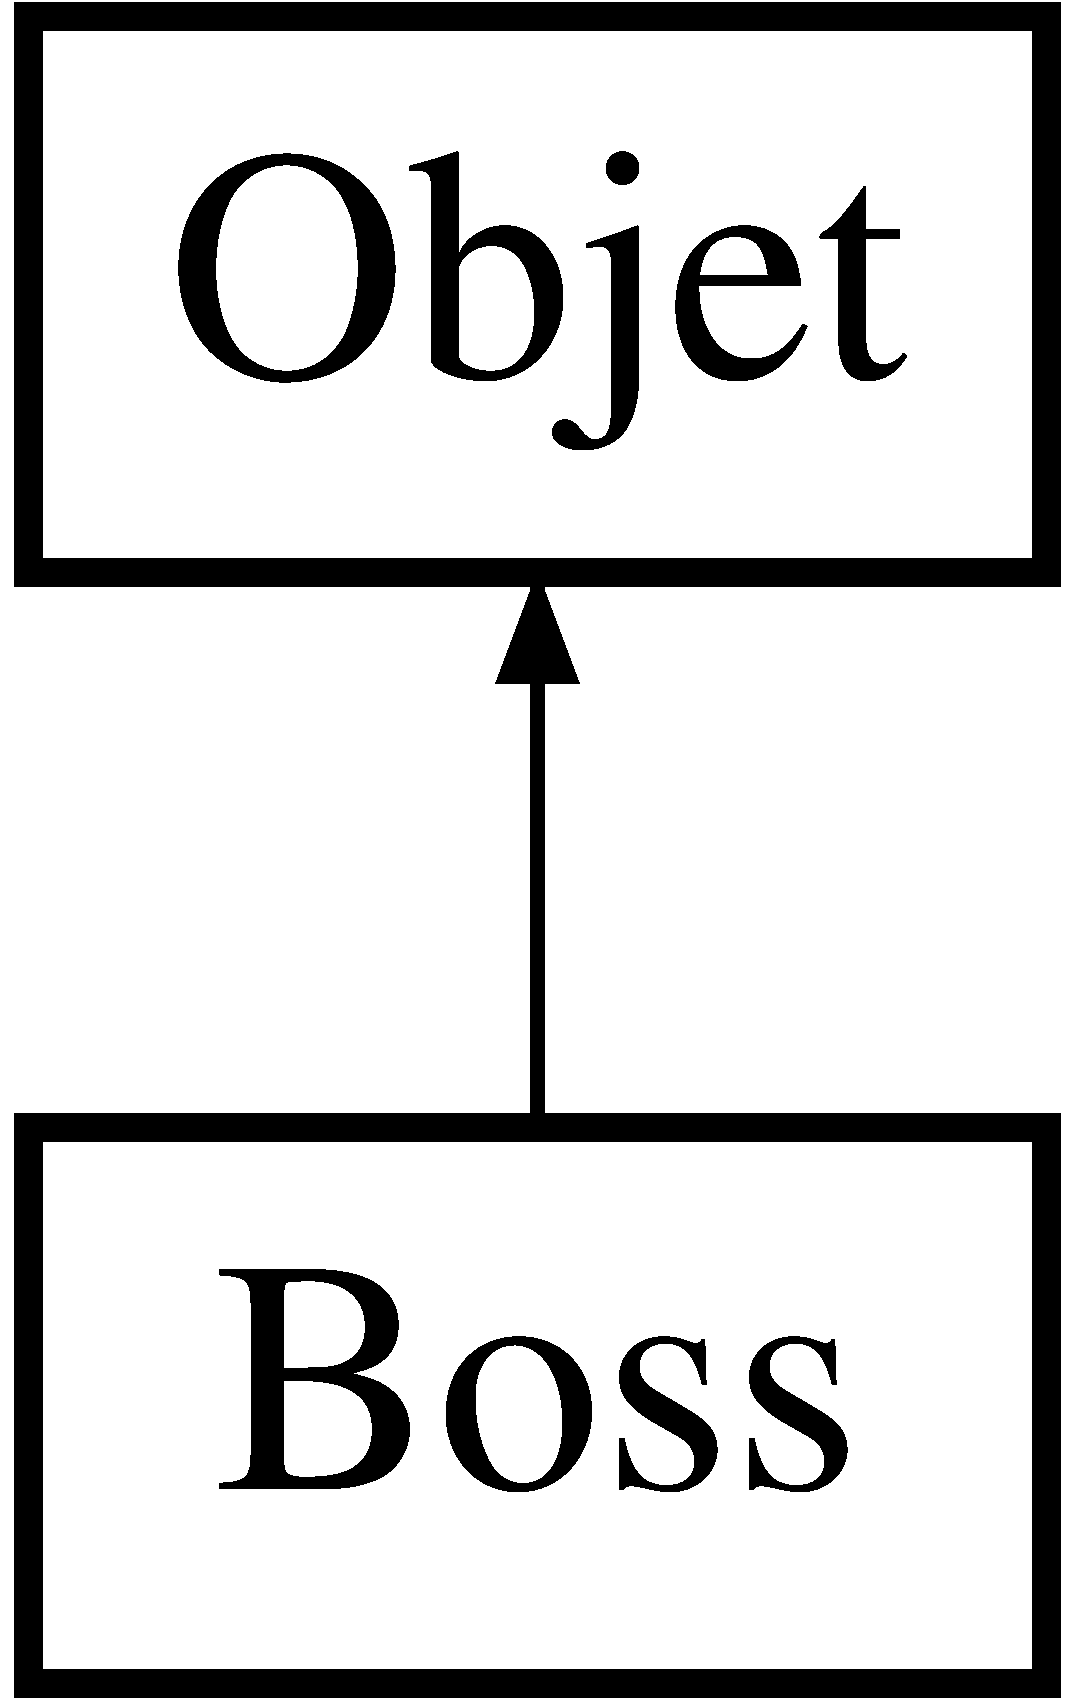
\includegraphics[height=2.000000cm]{class_boss}
\end{center}
\end{figure}
\subsection*{Fonctions membres publiques}
\begin{DoxyCompactItemize}
\item 
\hyperlink{class_boss_af287739a9fe8cb9501795656d34f3018}{Boss} ()
\item 
void \hyperlink{class_boss_ab3b0e756ba923f88c8afea3ed3af552c}{update} ()
\end{DoxyCompactItemize}
\subsection*{Membres hérités additionnels}


\subsection{Documentation des constructeurs et destructeur}
\mbox{\Hypertarget{class_boss_af287739a9fe8cb9501795656d34f3018}\label{class_boss_af287739a9fe8cb9501795656d34f3018}} 
\index{Boss@{Boss}!Boss@{Boss}}
\index{Boss@{Boss}!Boss@{Boss}}
\subsubsection{\texorpdfstring{Boss()}{Boss()}}
{\footnotesize\ttfamily Boss\+::\+Boss (\begin{DoxyParamCaption}{ }\end{DoxyParamCaption})\hspace{0.3cm}{\ttfamily [inline]}}



\subsection{Documentation des fonctions membres}
\mbox{\Hypertarget{class_boss_ab3b0e756ba923f88c8afea3ed3af552c}\label{class_boss_ab3b0e756ba923f88c8afea3ed3af552c}} 
\index{Boss@{Boss}!update@{update}}
\index{update@{update}!Boss@{Boss}}
\subsubsection{\texorpdfstring{update()}{update()}}
{\footnotesize\ttfamily void Boss\+::update (\begin{DoxyParamCaption}{ }\end{DoxyParamCaption})\hspace{0.3cm}{\ttfamily [inline]}, {\ttfamily [virtual]}}



Réimplémentée à partir de \hyperlink{class_objet_a684611b20eb6e6df5e4743dd3e42385a}{Objet}.



La documentation de cette classe a été générée à partir du fichier suivant \+:\begin{DoxyCompactItemize}
\item 
C\+:/\+Users/\+Ragnar\+L/\+Documents/p1408299-\/p1309837/\+Revenges\+Island/src/sfml/\hyperlink{_objet_8h}{Objet.\+h}\end{DoxyCompactItemize}

\hypertarget{class_ennemi}{}\section{Référence de la classe Ennemi}
\label{class_ennemi}\index{Ennemi@{Ennemi}}


classe utilisée pour la gestion de l\textquotesingle{}\hyperlink{class_ennemi}{Ennemi}. \hyperlink{class_ennemi}{Ennemi} hérite de la classe \hyperlink{class_object}{Object}.  




{\ttfamily \#include $<$Ennemi.\+h$>$}

Graphe d\textquotesingle{}héritage de Ennemi\+:\begin{figure}[H]
\begin{center}
\leavevmode
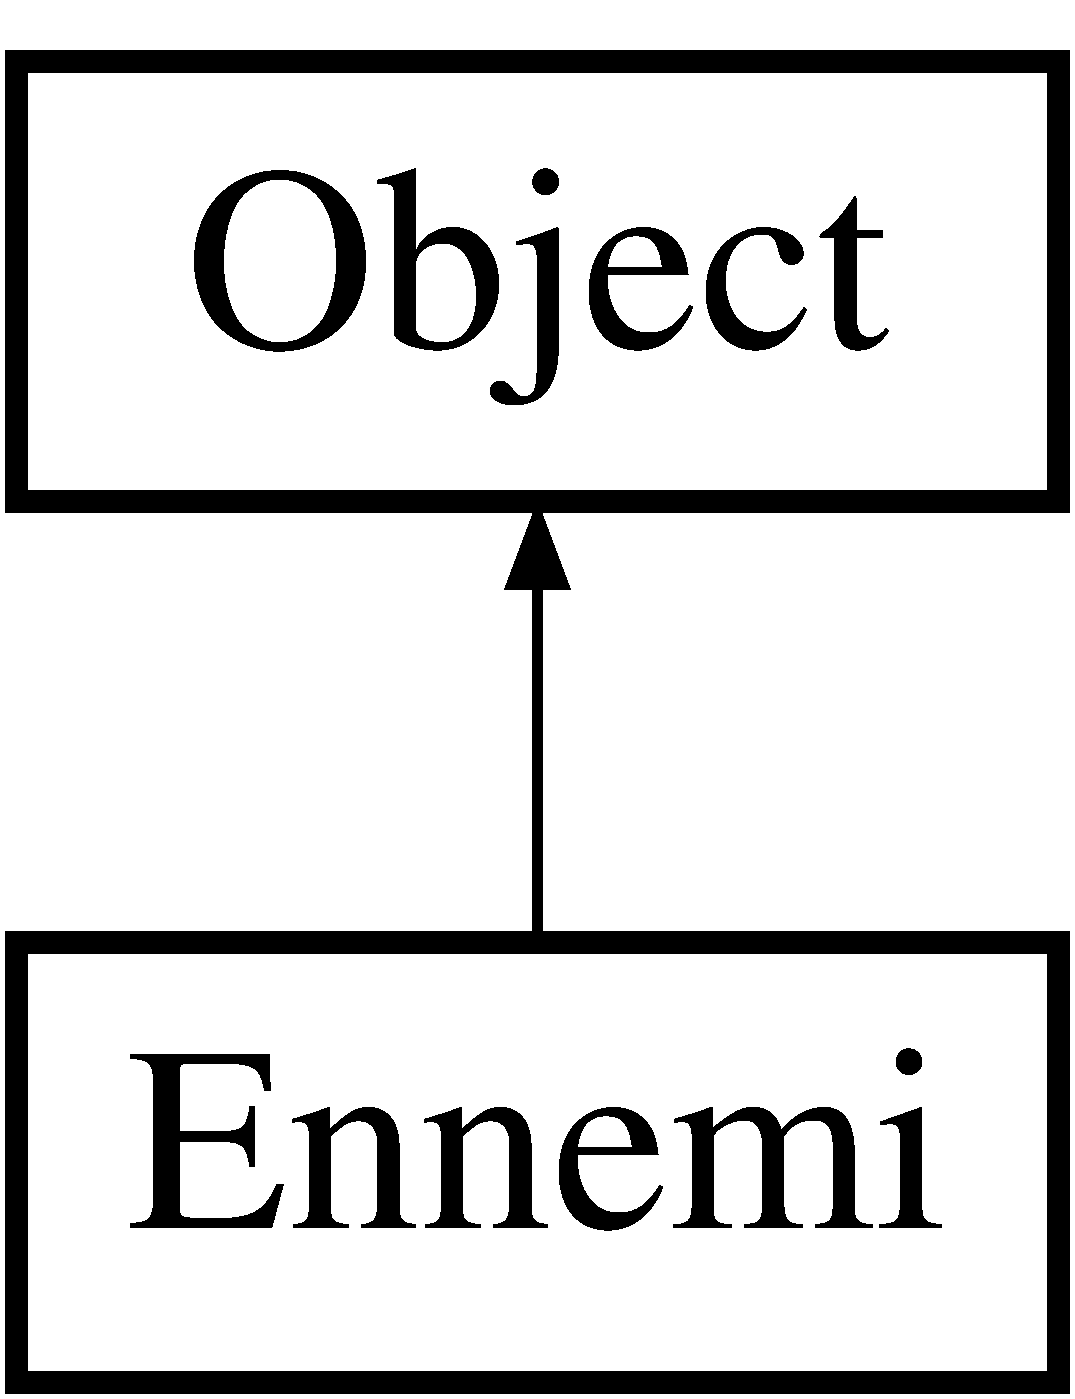
\includegraphics[height=2.000000cm]{class_ennemi}
\end{center}
\end{figure}
\subsection*{Fonctions membres publiques}
\begin{DoxyCompactItemize}
\item 
\hyperlink{class_ennemi_a9c5eb7ca82848b97f3dcf262fe625b3a}{Ennemi} ()
\begin{DoxyCompactList}\small\item\em Constructeur. \end{DoxyCompactList}\item 
void \hyperlink{class_ennemi_a649379ddaf7698276d924f48d56d87c5}{Deplace\+X\+Auto} (const \hyperlink{class_terrain}{Terrain} \&t)
\begin{DoxyCompactList}\small\item\em Deplace l\textquotesingle{}ennemi aléatoirement d\textquotesingle{}un cran en haut à gauche à droite ou à gauche. \end{DoxyCompactList}\item 
void \hyperlink{class_ennemi_a248d1bb99ad000f7dabbef353086ab1e}{Tir\+Auto} (\hyperlink{class_navigateur}{Navigateur} \&n, const \hyperlink{class_terrain}{Terrain} \&t, \hyperlink{class_shoot}{Shoot} \&be)
\begin{DoxyCompactList}\small\item\em Deplace le shoot de l\textquotesingle{}\hyperlink{class_ennemi}{Ennemi} sur la droite si il n\textquotesingle{}y pas d\textquotesingle{}obstacle et si les coordonnées du shoot et du \hyperlink{class_navigateur}{Navigateur} se rencontre, applique la gestion des points de vie au \hyperlink{class_navigateur}{Navigateur}. \end{DoxyCompactList}\end{DoxyCompactItemize}


\subsection{Description détaillée}
classe utilisée pour la gestion de l\textquotesingle{}\hyperlink{class_ennemi}{Ennemi}. \hyperlink{class_ennemi}{Ennemi} hérite de la classe \hyperlink{class_object}{Object}. 

\subsection{Documentation des constructeurs et destructeur}
\mbox{\Hypertarget{class_ennemi_a9c5eb7ca82848b97f3dcf262fe625b3a}\label{class_ennemi_a9c5eb7ca82848b97f3dcf262fe625b3a}} 
\index{Ennemi@{Ennemi}!Ennemi@{Ennemi}}
\index{Ennemi@{Ennemi}!Ennemi@{Ennemi}}
\subsubsection{\texorpdfstring{Ennemi()}{Ennemi()}}
{\footnotesize\ttfamily Ennemi\+::\+Ennemi (\begin{DoxyParamCaption}{ }\end{DoxyParamCaption})}



Constructeur. 

Constructeur par défaut de la classe \hyperlink{class_ennemi}{Ennemi} 

\subsection{Documentation des fonctions membres}
\mbox{\Hypertarget{class_ennemi_a649379ddaf7698276d924f48d56d87c5}\label{class_ennemi_a649379ddaf7698276d924f48d56d87c5}} 
\index{Ennemi@{Ennemi}!Deplace\+X\+Auto@{Deplace\+X\+Auto}}
\index{Deplace\+X\+Auto@{Deplace\+X\+Auto}!Ennemi@{Ennemi}}
\subsubsection{\texorpdfstring{Deplace\+X\+Auto()}{DeplaceXAuto()}}
{\footnotesize\ttfamily void Ennemi\+::\+Deplace\+X\+Auto (\begin{DoxyParamCaption}\item[{const \hyperlink{class_terrain}{Terrain} \&}]{t }\end{DoxyParamCaption})}



Deplace l\textquotesingle{}ennemi aléatoirement d\textquotesingle{}un cran en haut à gauche à droite ou à gauche. 


\begin{DoxyParams}{Paramètres}
{\em t} & \+: de type \hyperlink{class_terrain}{Terrain} \\
\hline
\end{DoxyParams}
\mbox{\Hypertarget{class_ennemi_a248d1bb99ad000f7dabbef353086ab1e}\label{class_ennemi_a248d1bb99ad000f7dabbef353086ab1e}} 
\index{Ennemi@{Ennemi}!Tir\+Auto@{Tir\+Auto}}
\index{Tir\+Auto@{Tir\+Auto}!Ennemi@{Ennemi}}
\subsubsection{\texorpdfstring{Tir\+Auto()}{TirAuto()}}
{\footnotesize\ttfamily void Ennemi\+::\+Tir\+Auto (\begin{DoxyParamCaption}\item[{\hyperlink{class_navigateur}{Navigateur} \&}]{n,  }\item[{const \hyperlink{class_terrain}{Terrain} \&}]{t,  }\item[{\hyperlink{class_shoot}{Shoot} \&}]{be }\end{DoxyParamCaption})}



Deplace le shoot de l\textquotesingle{}\hyperlink{class_ennemi}{Ennemi} sur la droite si il n\textquotesingle{}y pas d\textquotesingle{}obstacle et si les coordonnées du shoot et du \hyperlink{class_navigateur}{Navigateur} se rencontre, applique la gestion des points de vie au \hyperlink{class_navigateur}{Navigateur}. 


\begin{DoxyParams}{Paramètres}
{\em n} & \+: référence sur \hyperlink{class_navigateur}{Navigateur} \\
\hline
{\em t} & \+: de type \hyperlink{class_terrain}{Terrain} \\
\hline
{\em be} & \+: de type \hyperlink{class_shoot}{Shoot} \\
\hline
\end{DoxyParams}


La documentation de cette classe a été générée à partir des fichiers suivants \+:\begin{DoxyCompactItemize}
\item 
C\+:/\+Users/\+Ragnar\+L/\+Documents/p1408299-\/p1309837/\+Revenges\+Island/src/core/\hyperlink{_ennemi_8h}{Ennemi.\+h}\item 
C\+:/\+Users/\+Ragnar\+L/\+Documents/p1408299-\/p1309837/\+Revenges\+Island/src/core/\hyperlink{_ennemi_8cpp}{Ennemi.\+cpp}\end{DoxyCompactItemize}

\hypertarget{classennemi}{}\section{Référence de la classe ennemi}
\label{classennemi}\index{ennemi@{ennemi}}


{\ttfamily \#include $<$Objet.\+h$>$}

Graphe d\textquotesingle{}héritage de ennemi\+:\begin{figure}[H]
\begin{center}
\leavevmode
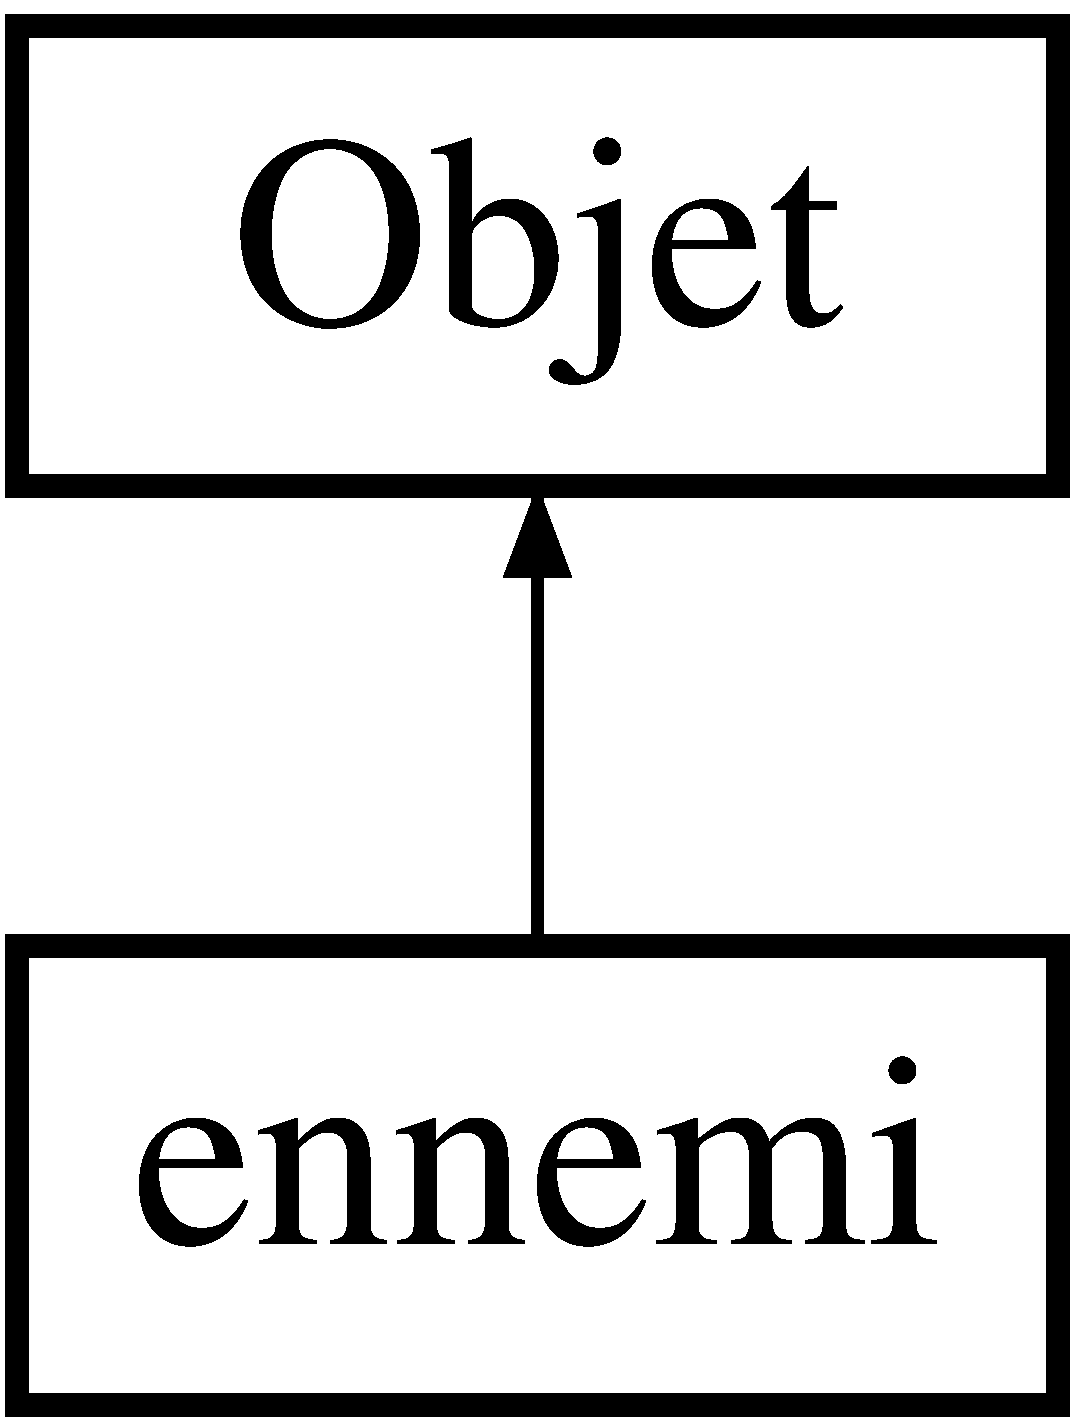
\includegraphics[height=2.000000cm]{classennemi}
\end{center}
\end{figure}
\subsection*{Fonctions membres publiques}
\begin{DoxyCompactItemize}
\item 
\hyperlink{classennemi_a7bd90d9f0e75fe07265e922a56b8a6c8}{ennemi} ()
\item 
void \hyperlink{classennemi_a52bb08c9e3c5597d0019857dc43f3351}{update} ()
\end{DoxyCompactItemize}
\subsection*{Membres hérités additionnels}


\subsection{Documentation des constructeurs et destructeur}
\mbox{\Hypertarget{classennemi_a7bd90d9f0e75fe07265e922a56b8a6c8}\label{classennemi_a7bd90d9f0e75fe07265e922a56b8a6c8}} 
\index{ennemi@{ennemi}!ennemi@{ennemi}}
\index{ennemi@{ennemi}!ennemi@{ennemi}}
\subsubsection{\texorpdfstring{ennemi()}{ennemi()}}
{\footnotesize\ttfamily ennemi\+::ennemi (\begin{DoxyParamCaption}{ }\end{DoxyParamCaption})\hspace{0.3cm}{\ttfamily [inline]}}



\subsection{Documentation des fonctions membres}
\mbox{\Hypertarget{classennemi_a52bb08c9e3c5597d0019857dc43f3351}\label{classennemi_a52bb08c9e3c5597d0019857dc43f3351}} 
\index{ennemi@{ennemi}!update@{update}}
\index{update@{update}!ennemi@{ennemi}}
\subsubsection{\texorpdfstring{update()}{update()}}
{\footnotesize\ttfamily void ennemi\+::update (\begin{DoxyParamCaption}{ }\end{DoxyParamCaption})\hspace{0.3cm}{\ttfamily [inline]}, {\ttfamily [virtual]}}



Réimplémentée à partir de \hyperlink{class_objet_a684611b20eb6e6df5e4743dd3e42385a}{Objet}.



La documentation de cette classe a été générée à partir du fichier suivant \+:\begin{DoxyCompactItemize}
\item 
C\+:/\+Users/\+Ragnar\+L/\+Documents/p1408299-\/p1309837/\+Revenges\+Island/src/sfml/\hyperlink{_objet_8h}{Objet.\+h}\end{DoxyCompactItemize}

\hypertarget{class_equipage}{}\section{Référence de la classe Equipage}
\label{class_equipage}\index{Equipage@{Equipage}}


classe utilisée pour la gestion de l\textquotesingle{}\hyperlink{class_equipage}{Equipage}. \hyperlink{class_equipage}{Equipage} hérite de la classe \hyperlink{class_object}{Object}.  




{\ttfamily \#include $<$Equipage.\+h$>$}

Graphe d\textquotesingle{}héritage de Equipage\+:\begin{figure}[H]
\begin{center}
\leavevmode
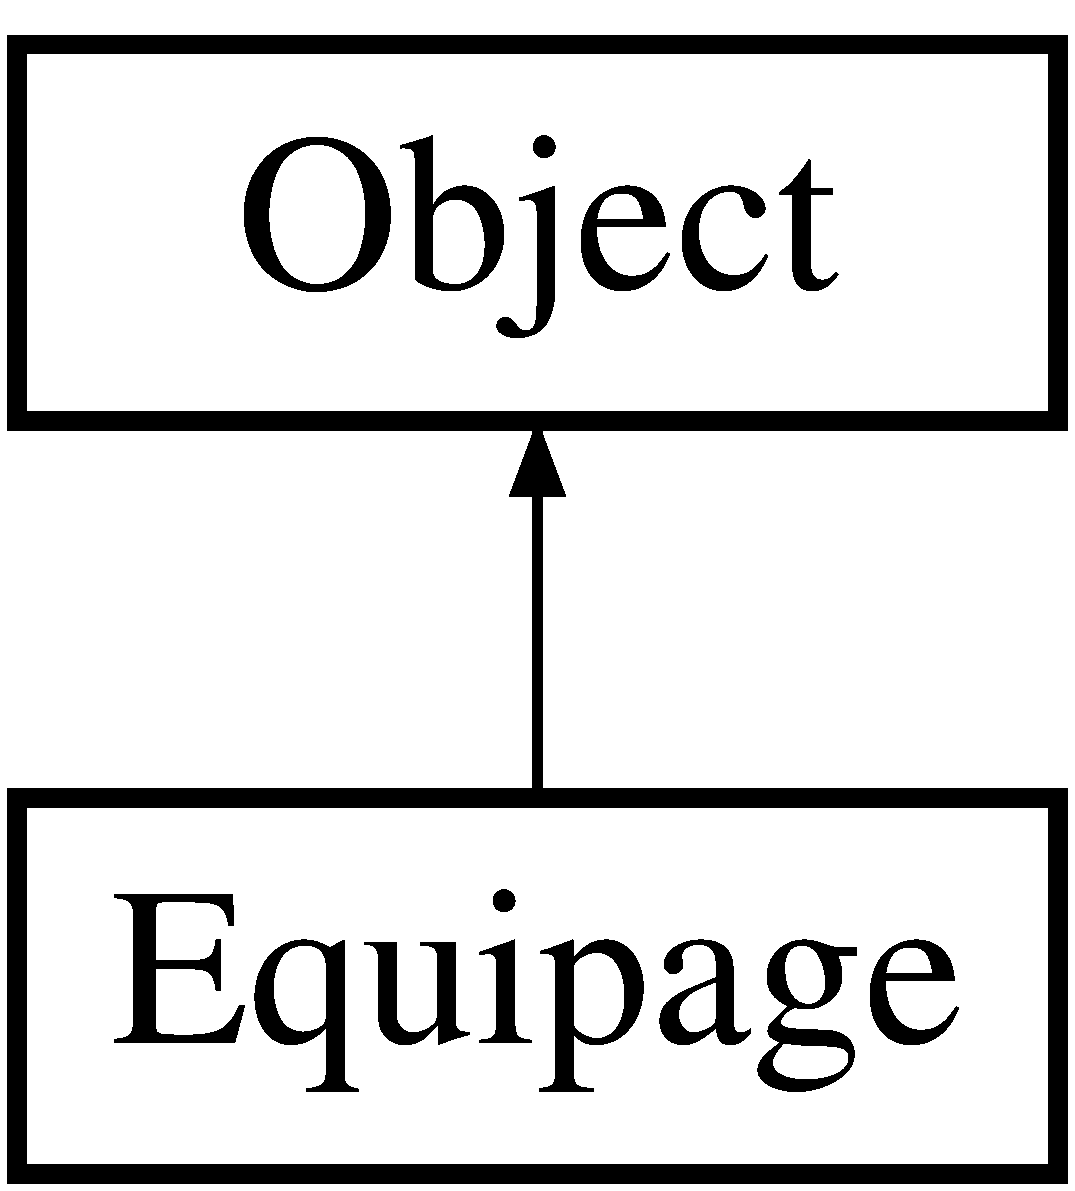
\includegraphics[height=2.000000cm]{class_equipage}
\end{center}
\end{figure}
\subsection*{Fonctions membres publiques}
\begin{DoxyCompactItemize}
\item 
\hyperlink{class_equipage_a25d4958c4ad1d69eebe6b4e434794e07}{Equipage} ()
\begin{DoxyCompactList}\small\item\em Constructeur. \end{DoxyCompactList}\item 
void \hyperlink{class_equipage_a2836ad0ea4c1f329ee3f9b88517f9d66}{Tir\+Allie} (\hyperlink{class_ennemi}{Ennemi} \&n, const \hyperlink{class_terrain}{Terrain} \&t, \hyperlink{class_shoot}{Shoot} \&balle)
\begin{DoxyCompactList}\small\item\em Deplace le shoot de l\textquotesingle{}\hyperlink{class_equipage}{Equipage} en direction de la dernière position de l\textquotesingle{}\hyperlink{class_ennemi}{Ennemi} et applique la collision sur celui-\/ci si elle a lieu. \end{DoxyCompactList}\end{DoxyCompactItemize}


\subsection{Description détaillée}
classe utilisée pour la gestion de l\textquotesingle{}\hyperlink{class_equipage}{Equipage}. \hyperlink{class_equipage}{Equipage} hérite de la classe \hyperlink{class_object}{Object}. 

\subsection{Documentation des constructeurs et destructeur}
\mbox{\Hypertarget{class_equipage_a25d4958c4ad1d69eebe6b4e434794e07}\label{class_equipage_a25d4958c4ad1d69eebe6b4e434794e07}} 
\index{Equipage@{Equipage}!Equipage@{Equipage}}
\index{Equipage@{Equipage}!Equipage@{Equipage}}
\subsubsection{\texorpdfstring{Equipage()}{Equipage()}}
{\footnotesize\ttfamily Equipage\+::\+Equipage (\begin{DoxyParamCaption}{ }\end{DoxyParamCaption})}



Constructeur. 

Constructeur par défaut de la classe \hyperlink{class_equipage}{Equipage} 

\subsection{Documentation des fonctions membres}
\mbox{\Hypertarget{class_equipage_a2836ad0ea4c1f329ee3f9b88517f9d66}\label{class_equipage_a2836ad0ea4c1f329ee3f9b88517f9d66}} 
\index{Equipage@{Equipage}!Tir\+Allie@{Tir\+Allie}}
\index{Tir\+Allie@{Tir\+Allie}!Equipage@{Equipage}}
\subsubsection{\texorpdfstring{Tir\+Allie()}{TirAllie()}}
{\footnotesize\ttfamily void Equipage\+::\+Tir\+Allie (\begin{DoxyParamCaption}\item[{\hyperlink{class_ennemi}{Ennemi} \&}]{n,  }\item[{const \hyperlink{class_terrain}{Terrain} \&}]{t,  }\item[{\hyperlink{class_shoot}{Shoot} \&}]{balle }\end{DoxyParamCaption})}



Deplace le shoot de l\textquotesingle{}\hyperlink{class_equipage}{Equipage} en direction de la dernière position de l\textquotesingle{}\hyperlink{class_ennemi}{Ennemi} et applique la collision sur celui-\/ci si elle a lieu. 


\begin{DoxyParams}{Paramètres}
{\em n} & \+: référence sur \hyperlink{class_ennemi}{Ennemi} \\
\hline
{\em t} & \+: de type \hyperlink{class_terrain}{Terrain} \\
\hline
{\em balle} & \+: de type \hyperlink{class_shoot}{Shoot} \\
\hline
\end{DoxyParams}


La documentation de cette classe a été générée à partir des fichiers suivants \+:\begin{DoxyCompactItemize}
\item 
C\+:/\+Users/\+Ragnar\+L/\+Documents/p1408299-\/p1309837/\+Revenges\+Island/src/core/\hyperlink{_equipage_8h}{Equipage.\+h}\item 
C\+:/\+Users/\+Ragnar\+L/\+Documents/p1408299-\/p1309837/\+Revenges\+Island/src/core/\hyperlink{_equipage_8cpp}{Equipage.\+cpp}\end{DoxyCompactItemize}

\hypertarget{classhache}{}\section{Référence de la classe hache}
\label{classhache}\index{hache@{hache}}


{\ttfamily \#include $<$Objet.\+h$>$}

Graphe d\textquotesingle{}héritage de hache\+:\begin{figure}[H]
\begin{center}
\leavevmode
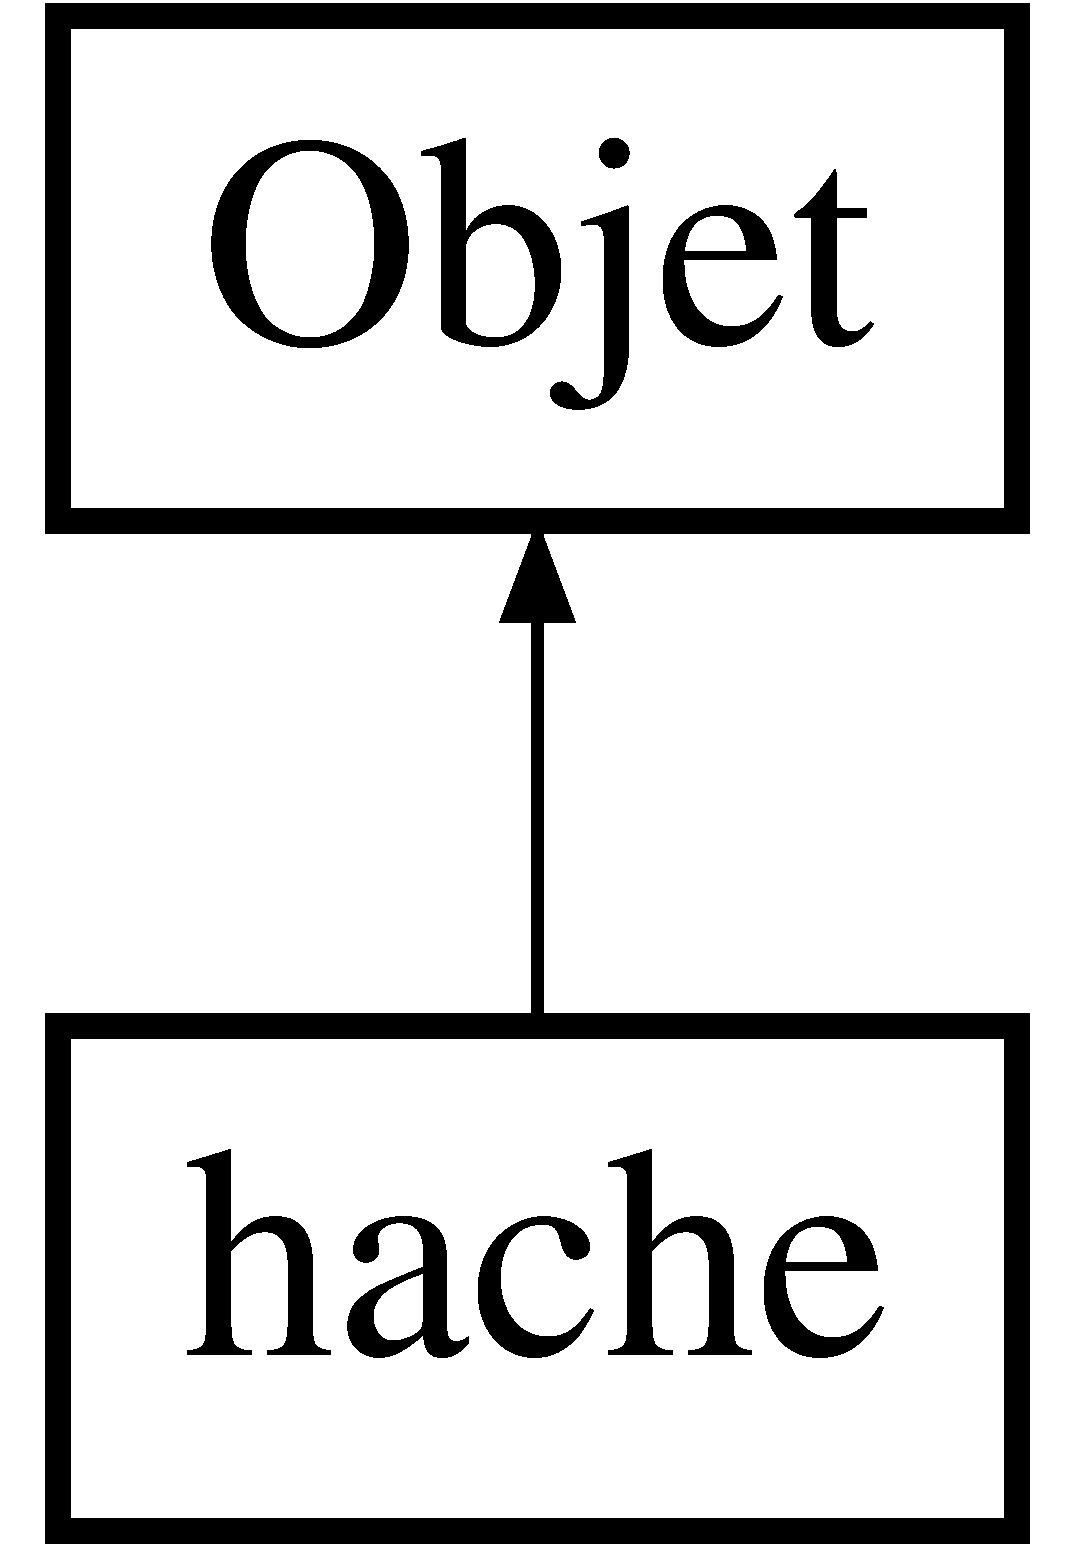
\includegraphics[height=2.000000cm]{classhache}
\end{center}
\end{figure}
\subsection*{Fonctions membres publiques}
\begin{DoxyCompactItemize}
\item 
\hyperlink{classhache_aa48ac7a5b20fb97e50b49b8d02915b13}{hache} ()
\item 
void \hyperlink{classhache_a0b491958a8b90c3f6cc79e28e094a410}{update} ()
\end{DoxyCompactItemize}
\subsection*{Membres hérités additionnels}


\subsection{Documentation des constructeurs et destructeur}
\mbox{\Hypertarget{classhache_aa48ac7a5b20fb97e50b49b8d02915b13}\label{classhache_aa48ac7a5b20fb97e50b49b8d02915b13}} 
\index{hache@{hache}!hache@{hache}}
\index{hache@{hache}!hache@{hache}}
\subsubsection{\texorpdfstring{hache()}{hache()}}
{\footnotesize\ttfamily hache\+::hache (\begin{DoxyParamCaption}{ }\end{DoxyParamCaption})\hspace{0.3cm}{\ttfamily [inline]}}



\subsection{Documentation des fonctions membres}
\mbox{\Hypertarget{classhache_a0b491958a8b90c3f6cc79e28e094a410}\label{classhache_a0b491958a8b90c3f6cc79e28e094a410}} 
\index{hache@{hache}!update@{update}}
\index{update@{update}!hache@{hache}}
\subsubsection{\texorpdfstring{update()}{update()}}
{\footnotesize\ttfamily void hache\+::update (\begin{DoxyParamCaption}{ }\end{DoxyParamCaption})\hspace{0.3cm}{\ttfamily [inline]}, {\ttfamily [virtual]}}



Réimplémentée à partir de \hyperlink{class_objet_a684611b20eb6e6df5e4743dd3e42385a}{Objet}.



La documentation de cette classe a été générée à partir du fichier suivant \+:\begin{DoxyCompactItemize}
\item 
C\+:/\+Users/\+Ragnar\+L/\+Documents/p1408299-\/p1309837/\+Revenges\+Island/src/sfml/\hyperlink{_objet_8h}{Objet.\+h}\end{DoxyCompactItemize}

\hypertarget{class_image}{}\section{Référence de la classe Image}
\label{class_image}\index{Image@{Image}}


Pour g�rer une image avec S\+D\+L2.  




{\ttfamily \#include $<$sdl\+Jeu.\+h$>$}

\subsection*{Fonctions membres publiques}
\begin{DoxyCompactItemize}
\item 
\hyperlink{class_image_a58edd1c45b4faeb5f789b0d036d02313}{Image} ()
\item 
void \hyperlink{class_image_aa276b5183099671ddeaf8f083068046c}{load\+From\+File} (const char $\ast$filename, S\+D\+L\+\_\+\+Renderer $\ast$renderer)
\item 
void \hyperlink{class_image_a82d6936d466ba0161d8b9cbacf613de5}{draw} (S\+D\+L\+\_\+\+Renderer $\ast$renderer, int x, int y, int w=-\/1, int h=-\/1)
\end{DoxyCompactItemize}
\subsection*{Attributs privés}
\begin{DoxyCompactItemize}
\item 
S\+D\+L\+\_\+\+Surface $\ast$ \hyperlink{class_image_ac1d365143f4f5ee59f318977ad6d798b}{surface}
\item 
S\+D\+L\+\_\+\+Texture $\ast$ \hyperlink{class_image_a4f44588a7d341e02dae82e2de94dfad6}{texture}
\item 
bool \hyperlink{class_image_ab4cb83faeecef0cfb2773813c4757b45}{has\+\_\+changed}
\end{DoxyCompactItemize}


\subsection{Description détaillée}
Pour g�rer une image avec S\+D\+L2. 

\subsection{Documentation des constructeurs et destructeur}
\mbox{\Hypertarget{class_image_a58edd1c45b4faeb5f789b0d036d02313}\label{class_image_a58edd1c45b4faeb5f789b0d036d02313}} 
\index{Image@{Image}!Image@{Image}}
\index{Image@{Image}!Image@{Image}}
\subsubsection{\texorpdfstring{Image()}{Image()}}
{\footnotesize\ttfamily Image\+::\+Image (\begin{DoxyParamCaption}{ }\end{DoxyParamCaption})}



\subsection{Documentation des fonctions membres}
\mbox{\Hypertarget{class_image_a82d6936d466ba0161d8b9cbacf613de5}\label{class_image_a82d6936d466ba0161d8b9cbacf613de5}} 
\index{Image@{Image}!draw@{draw}}
\index{draw@{draw}!Image@{Image}}
\subsubsection{\texorpdfstring{draw()}{draw()}}
{\footnotesize\ttfamily void Image\+::draw (\begin{DoxyParamCaption}\item[{S\+D\+L\+\_\+\+Renderer $\ast$}]{renderer,  }\item[{int}]{x,  }\item[{int}]{y,  }\item[{int}]{w = {\ttfamily -\/1},  }\item[{int}]{h = {\ttfamily -\/1} }\end{DoxyParamCaption})}

\mbox{\Hypertarget{class_image_aa276b5183099671ddeaf8f083068046c}\label{class_image_aa276b5183099671ddeaf8f083068046c}} 
\index{Image@{Image}!load\+From\+File@{load\+From\+File}}
\index{load\+From\+File@{load\+From\+File}!Image@{Image}}
\subsubsection{\texorpdfstring{load\+From\+File()}{loadFromFile()}}
{\footnotesize\ttfamily void Image\+::load\+From\+File (\begin{DoxyParamCaption}\item[{const char $\ast$}]{filename,  }\item[{S\+D\+L\+\_\+\+Renderer $\ast$}]{renderer }\end{DoxyParamCaption})}



\subsection{Documentation des données membres}
\mbox{\Hypertarget{class_image_ab4cb83faeecef0cfb2773813c4757b45}\label{class_image_ab4cb83faeecef0cfb2773813c4757b45}} 
\index{Image@{Image}!has\+\_\+changed@{has\+\_\+changed}}
\index{has\+\_\+changed@{has\+\_\+changed}!Image@{Image}}
\subsubsection{\texorpdfstring{has\+\_\+changed}{has\_changed}}
{\footnotesize\ttfamily bool Image\+::has\+\_\+changed\hspace{0.3cm}{\ttfamily [private]}}

\mbox{\Hypertarget{class_image_ac1d365143f4f5ee59f318977ad6d798b}\label{class_image_ac1d365143f4f5ee59f318977ad6d798b}} 
\index{Image@{Image}!surface@{surface}}
\index{surface@{surface}!Image@{Image}}
\subsubsection{\texorpdfstring{surface}{surface}}
{\footnotesize\ttfamily S\+D\+L\+\_\+\+Surface$\ast$ Image\+::surface\hspace{0.3cm}{\ttfamily [private]}}

\mbox{\Hypertarget{class_image_a4f44588a7d341e02dae82e2de94dfad6}\label{class_image_a4f44588a7d341e02dae82e2de94dfad6}} 
\index{Image@{Image}!texture@{texture}}
\index{texture@{texture}!Image@{Image}}
\subsubsection{\texorpdfstring{texture}{texture}}
{\footnotesize\ttfamily S\+D\+L\+\_\+\+Texture$\ast$ Image\+::texture\hspace{0.3cm}{\ttfamily [private]}}



La documentation de cette classe a été générée à partir des fichiers suivants \+:\begin{DoxyCompactItemize}
\item 
C\+:/\+Users/\+Ragnar\+L/\+Documents/p1408299-\/p1309837/\+Revenges\+Island/src/sdl2/\hyperlink{sdl_jeu_8h}{sdl\+Jeu.\+h}\item 
C\+:/\+Users/\+Ragnar\+L/\+Documents/p1408299-\/p1309837/\+Revenges\+Island/src/sdl2/\hyperlink{sdl_jeu_8cpp}{sdl\+Jeu.\+cpp}\end{DoxyCompactItemize}

\hypertarget{class_jeu}{}\section{Référence de la classe Jeu}
\label{class_jeu}\index{Jeu@{Jeu}}


{\ttfamily \#include $<$Jeu.\+h$>$}

\subsection*{Fonctions membres publiques}
\begin{DoxyCompactItemize}
\item 
\hyperlink{class_jeu_acc5795ee00edf75516d3dfe65be3e6d6}{Jeu} ()
\begin{DoxyCompactList}\small\item\em Constructeur. \end{DoxyCompactList}\item 
const \hyperlink{class_terrain}{Terrain} \& \hyperlink{class_jeu_af7e7bd59e117f78b9d8623fd76230ca3}{get\+Const\+Terrain} () const
\begin{DoxyCompactList}\small\item\em Accesseur de la class \hyperlink{class_jeu}{Jeu}. \end{DoxyCompactList}\item 
const \hyperlink{class_navigateur}{Navigateur} \& \hyperlink{class_jeu_af2d070e73c6c9bd9dc3cf09d110a82eb}{get\+Const\+Navigateur} () const
\begin{DoxyCompactList}\small\item\em Accesseur de la class \hyperlink{class_jeu}{Jeu}. \end{DoxyCompactList}\item 
const \hyperlink{class_ennemi}{Ennemi} \& \hyperlink{class_jeu_a9266f571dc8cfacdf01e6f13d8a13568}{get\+Const\+Ennemi} () const
\begin{DoxyCompactList}\small\item\em Accesseur de la class \hyperlink{class_jeu}{Jeu}. \end{DoxyCompactList}\item 
const \hyperlink{class_equipage}{Equipage} \& \hyperlink{class_jeu_a8831cd95b6bf8984712e212a9db537cf}{get\+Const\+Equipage} () const
\begin{DoxyCompactList}\small\item\em Accesseur de la class \hyperlink{class_jeu}{Jeu}. \end{DoxyCompactList}\item 
const \hyperlink{class_shoot}{Shoot} \& \hyperlink{class_jeu_af71805735942a00e774ab906a3019ddf}{get\+Constshoot\+Nav} () const
\begin{DoxyCompactList}\small\item\em Accesseur de la class \hyperlink{class_jeu}{Jeu}. \end{DoxyCompactList}\item 
const \hyperlink{class_shoot}{Shoot} \& \hyperlink{class_jeu_ae864beb5c3c85c1d152dedf39c838254}{get\+Constshoot\+En} () const
\begin{DoxyCompactList}\small\item\em Accesseur de la class \hyperlink{class_jeu}{Jeu}. \end{DoxyCompactList}\item 
const \hyperlink{class_shoot}{Shoot} \& \hyperlink{class_jeu_ac305ed7d05845e93da364408ddf23f7a}{get\+Constshoot\+Eq} () const
\begin{DoxyCompactList}\small\item\em Accesseur de la class \hyperlink{class_jeu}{Jeu}. \end{DoxyCompactList}\item 
void \hyperlink{class_jeu_a849e140df1504ddfd1e1eccc4374718f}{actions\+Automatiques} ()
\begin{DoxyCompactList}\small\item\em Enclenche un deplacement aléatoire de l\textquotesingle{}ennemi, et un shoot de l\textquotesingle{}ennemi, du navigateur et de l\textquotesingle{}équipage. \end{DoxyCompactList}\item 
void \hyperlink{class_jeu_ab27fb1db9e2ae2a0c19a90ecc838319f}{action\+Clavier} (const char touche)
\begin{DoxyCompactList}\small\item\em Attribue des touches du claviers au mouvement du navigateur. \end{DoxyCompactList}\item 
void \hyperlink{class_jeu_aa00e3f0a90d6b38c83c16700cdd15190}{changer\+Niveau} ()
\begin{DoxyCompactList}\small\item\em Enclenche un changement de terrain lorsque le navigateur gagne un niveau. \end{DoxyCompactList}\end{DoxyCompactItemize}
\subsection*{Attributs privés}
\begin{DoxyCompactItemize}
\item 
\hyperlink{class_navigateur}{Navigateur} \hyperlink{class_jeu_a0ad4c146ac99e95600bdcfd55a13236c}{nav}
\item 
\hyperlink{class_ennemi}{Ennemi} \hyperlink{class_jeu_ab0d2c6597c665841833d051a05f8ba92}{en}
\item 
\hyperlink{class_equipage}{Equipage} \hyperlink{class_jeu_a558e9bff3ccad86850b319f7b95291c0}{eq}
\item 
\hyperlink{class_shoot}{Shoot} \hyperlink{class_jeu_ae29392e165aa69c1b841753b6b1b7b5e}{shoot\+Nav}
\item 
\hyperlink{class_shoot}{Shoot} \hyperlink{class_jeu_a66b2ea36a3649c7faf88fca2f07bdc97}{shoot\+En}
\item 
\hyperlink{class_shoot}{Shoot} \hyperlink{class_jeu_a07e0707082701c5d3306f1659028c3c1}{shoot\+Eq}
\item 
\hyperlink{class_terrain}{Terrain} \hyperlink{class_jeu_a6ef0d2feb24c59b28fe08059057e96ff}{ter}
\end{DoxyCompactItemize}


\subsection{Description détaillée}

\begin{DoxyParams}[1]{Paramètres}
\mbox{\tt in}  & {\em nav} & \hyperlink{class_navigateur}{Navigateur} \\
\hline
\mbox{\tt in}  & {\em en} & \hyperlink{class_ennemi}{Ennemi} \\
\hline
\mbox{\tt in}  & {\em eq} & \hyperlink{class_equipage}{Equipage} \\
\hline
\mbox{\tt in}  & {\em shoot\+Nav} & \hyperlink{class_shoot}{Shoot} du \hyperlink{class_navigateur}{Navigateur} \\
\hline
\mbox{\tt in}  & {\em shoot\+En} & \hyperlink{class_shoot}{Shoot} de l\textquotesingle{}\hyperlink{class_ennemi}{Ennemi} \\
\hline
\mbox{\tt in}  & {\em shoot\+Eq} & \hyperlink{class_shoot}{Shoot} de l\textquotesingle{}\hyperlink{class_equipage}{Equipage} \\
\hline
\mbox{\tt in}  & {\em ter} & \hyperlink{class_terrain}{Terrain} \\
\hline
\end{DoxyParams}


\subsection{Documentation des constructeurs et destructeur}
\mbox{\Hypertarget{class_jeu_acc5795ee00edf75516d3dfe65be3e6d6}\label{class_jeu_acc5795ee00edf75516d3dfe65be3e6d6}} 
\index{Jeu@{Jeu}!Jeu@{Jeu}}
\index{Jeu@{Jeu}!Jeu@{Jeu}}
\subsubsection{\texorpdfstring{Jeu()}{Jeu()}}
{\footnotesize\ttfamily Jeu\+::\+Jeu (\begin{DoxyParamCaption}{ }\end{DoxyParamCaption})}



Constructeur. 

Constructeur par défaut de la classe \hyperlink{class_jeu}{Jeu} 

\subsection{Documentation des fonctions membres}
\mbox{\Hypertarget{class_jeu_ab27fb1db9e2ae2a0c19a90ecc838319f}\label{class_jeu_ab27fb1db9e2ae2a0c19a90ecc838319f}} 
\index{Jeu@{Jeu}!action\+Clavier@{action\+Clavier}}
\index{action\+Clavier@{action\+Clavier}!Jeu@{Jeu}}
\subsubsection{\texorpdfstring{action\+Clavier()}{actionClavier()}}
{\footnotesize\ttfamily void Jeu\+::action\+Clavier (\begin{DoxyParamCaption}\item[{const char}]{touche }\end{DoxyParamCaption})}



Attribue des touches du claviers au mouvement du navigateur. 


\begin{DoxyParams}{Paramètres}
{\em touche} & \+: un caractère \\
\hline
\end{DoxyParams}
\mbox{\Hypertarget{class_jeu_a849e140df1504ddfd1e1eccc4374718f}\label{class_jeu_a849e140df1504ddfd1e1eccc4374718f}} 
\index{Jeu@{Jeu}!actions\+Automatiques@{actions\+Automatiques}}
\index{actions\+Automatiques@{actions\+Automatiques}!Jeu@{Jeu}}
\subsubsection{\texorpdfstring{actions\+Automatiques()}{actionsAutomatiques()}}
{\footnotesize\ttfamily void Jeu\+::actions\+Automatiques (\begin{DoxyParamCaption}{ }\end{DoxyParamCaption})}



Enclenche un deplacement aléatoire de l\textquotesingle{}ennemi, et un shoot de l\textquotesingle{}ennemi, du navigateur et de l\textquotesingle{}équipage. 

\mbox{\Hypertarget{class_jeu_aa00e3f0a90d6b38c83c16700cdd15190}\label{class_jeu_aa00e3f0a90d6b38c83c16700cdd15190}} 
\index{Jeu@{Jeu}!changer\+Niveau@{changer\+Niveau}}
\index{changer\+Niveau@{changer\+Niveau}!Jeu@{Jeu}}
\subsubsection{\texorpdfstring{changer\+Niveau()}{changerNiveau()}}
{\footnotesize\ttfamily void Jeu\+::changer\+Niveau (\begin{DoxyParamCaption}{ }\end{DoxyParamCaption})}



Enclenche un changement de terrain lorsque le navigateur gagne un niveau. 

\mbox{\Hypertarget{class_jeu_a9266f571dc8cfacdf01e6f13d8a13568}\label{class_jeu_a9266f571dc8cfacdf01e6f13d8a13568}} 
\index{Jeu@{Jeu}!get\+Const\+Ennemi@{get\+Const\+Ennemi}}
\index{get\+Const\+Ennemi@{get\+Const\+Ennemi}!Jeu@{Jeu}}
\subsubsection{\texorpdfstring{get\+Const\+Ennemi()}{getConstEnnemi()}}
{\footnotesize\ttfamily const \hyperlink{class_ennemi}{Ennemi} \& Jeu\+::get\+Const\+Ennemi (\begin{DoxyParamCaption}{ }\end{DoxyParamCaption}) const}



Accesseur de la class \hyperlink{class_jeu}{Jeu}. 

\hyperlink{class_terrain}{Terrain}\& get\+Const\+Ennemi () const; \mbox{\Hypertarget{class_jeu_a8831cd95b6bf8984712e212a9db537cf}\label{class_jeu_a8831cd95b6bf8984712e212a9db537cf}} 
\index{Jeu@{Jeu}!get\+Const\+Equipage@{get\+Const\+Equipage}}
\index{get\+Const\+Equipage@{get\+Const\+Equipage}!Jeu@{Jeu}}
\subsubsection{\texorpdfstring{get\+Const\+Equipage()}{getConstEquipage()}}
{\footnotesize\ttfamily const \hyperlink{class_equipage}{Equipage} \& Jeu\+::get\+Const\+Equipage (\begin{DoxyParamCaption}{ }\end{DoxyParamCaption}) const}



Accesseur de la class \hyperlink{class_jeu}{Jeu}. 

\hyperlink{class_terrain}{Terrain}\& get\+Const\+Equipage () const; \mbox{\Hypertarget{class_jeu_af2d070e73c6c9bd9dc3cf09d110a82eb}\label{class_jeu_af2d070e73c6c9bd9dc3cf09d110a82eb}} 
\index{Jeu@{Jeu}!get\+Const\+Navigateur@{get\+Const\+Navigateur}}
\index{get\+Const\+Navigateur@{get\+Const\+Navigateur}!Jeu@{Jeu}}
\subsubsection{\texorpdfstring{get\+Const\+Navigateur()}{getConstNavigateur()}}
{\footnotesize\ttfamily const \hyperlink{class_navigateur}{Navigateur} \& Jeu\+::get\+Const\+Navigateur (\begin{DoxyParamCaption}{ }\end{DoxyParamCaption}) const}



Accesseur de la class \hyperlink{class_jeu}{Jeu}. 

\hyperlink{class_terrain}{Terrain}\& get\+Const\+Navigateur () const; \mbox{\Hypertarget{class_jeu_ae864beb5c3c85c1d152dedf39c838254}\label{class_jeu_ae864beb5c3c85c1d152dedf39c838254}} 
\index{Jeu@{Jeu}!get\+Constshoot\+En@{get\+Constshoot\+En}}
\index{get\+Constshoot\+En@{get\+Constshoot\+En}!Jeu@{Jeu}}
\subsubsection{\texorpdfstring{get\+Constshoot\+En()}{getConstshootEn()}}
{\footnotesize\ttfamily const \hyperlink{class_shoot}{Shoot} \& Jeu\+::get\+Constshoot\+En (\begin{DoxyParamCaption}{ }\end{DoxyParamCaption}) const}



Accesseur de la class \hyperlink{class_jeu}{Jeu}. 

\hyperlink{class_terrain}{Terrain}\& get\+Constshoot\+En () const; \mbox{\Hypertarget{class_jeu_ac305ed7d05845e93da364408ddf23f7a}\label{class_jeu_ac305ed7d05845e93da364408ddf23f7a}} 
\index{Jeu@{Jeu}!get\+Constshoot\+Eq@{get\+Constshoot\+Eq}}
\index{get\+Constshoot\+Eq@{get\+Constshoot\+Eq}!Jeu@{Jeu}}
\subsubsection{\texorpdfstring{get\+Constshoot\+Eq()}{getConstshootEq()}}
{\footnotesize\ttfamily const \hyperlink{class_shoot}{Shoot} \& Jeu\+::get\+Constshoot\+Eq (\begin{DoxyParamCaption}{ }\end{DoxyParamCaption}) const}



Accesseur de la class \hyperlink{class_jeu}{Jeu}. 

\hyperlink{class_terrain}{Terrain}\& get\+Constshoot\+Eq () const; \mbox{\Hypertarget{class_jeu_af71805735942a00e774ab906a3019ddf}\label{class_jeu_af71805735942a00e774ab906a3019ddf}} 
\index{Jeu@{Jeu}!get\+Constshoot\+Nav@{get\+Constshoot\+Nav}}
\index{get\+Constshoot\+Nav@{get\+Constshoot\+Nav}!Jeu@{Jeu}}
\subsubsection{\texorpdfstring{get\+Constshoot\+Nav()}{getConstshootNav()}}
{\footnotesize\ttfamily const \hyperlink{class_shoot}{Shoot} \& Jeu\+::get\+Constshoot\+Nav (\begin{DoxyParamCaption}{ }\end{DoxyParamCaption}) const}



Accesseur de la class \hyperlink{class_jeu}{Jeu}. 

\hyperlink{class_terrain}{Terrain}\& get\+Constshoot\+Nav () const; \mbox{\Hypertarget{class_jeu_af7e7bd59e117f78b9d8623fd76230ca3}\label{class_jeu_af7e7bd59e117f78b9d8623fd76230ca3}} 
\index{Jeu@{Jeu}!get\+Const\+Terrain@{get\+Const\+Terrain}}
\index{get\+Const\+Terrain@{get\+Const\+Terrain}!Jeu@{Jeu}}
\subsubsection{\texorpdfstring{get\+Const\+Terrain()}{getConstTerrain()}}
{\footnotesize\ttfamily const \hyperlink{class_terrain}{Terrain} \& Jeu\+::get\+Const\+Terrain (\begin{DoxyParamCaption}{ }\end{DoxyParamCaption}) const}



Accesseur de la class \hyperlink{class_jeu}{Jeu}. 

\hyperlink{class_terrain}{Terrain}\& get\+Const\+Terrain () const; 

\subsection{Documentation des données membres}
\mbox{\Hypertarget{class_jeu_ab0d2c6597c665841833d051a05f8ba92}\label{class_jeu_ab0d2c6597c665841833d051a05f8ba92}} 
\index{Jeu@{Jeu}!en@{en}}
\index{en@{en}!Jeu@{Jeu}}
\subsubsection{\texorpdfstring{en}{en}}
{\footnotesize\ttfamily \hyperlink{class_ennemi}{Ennemi} Jeu\+::en\hspace{0.3cm}{\ttfamily [private]}}

\mbox{\Hypertarget{class_jeu_a558e9bff3ccad86850b319f7b95291c0}\label{class_jeu_a558e9bff3ccad86850b319f7b95291c0}} 
\index{Jeu@{Jeu}!eq@{eq}}
\index{eq@{eq}!Jeu@{Jeu}}
\subsubsection{\texorpdfstring{eq}{eq}}
{\footnotesize\ttfamily \hyperlink{class_equipage}{Equipage} Jeu\+::eq\hspace{0.3cm}{\ttfamily [private]}}

\mbox{\Hypertarget{class_jeu_a0ad4c146ac99e95600bdcfd55a13236c}\label{class_jeu_a0ad4c146ac99e95600bdcfd55a13236c}} 
\index{Jeu@{Jeu}!nav@{nav}}
\index{nav@{nav}!Jeu@{Jeu}}
\subsubsection{\texorpdfstring{nav}{nav}}
{\footnotesize\ttfamily \hyperlink{class_navigateur}{Navigateur} Jeu\+::nav\hspace{0.3cm}{\ttfamily [private]}}

\mbox{\Hypertarget{class_jeu_a66b2ea36a3649c7faf88fca2f07bdc97}\label{class_jeu_a66b2ea36a3649c7faf88fca2f07bdc97}} 
\index{Jeu@{Jeu}!shoot\+En@{shoot\+En}}
\index{shoot\+En@{shoot\+En}!Jeu@{Jeu}}
\subsubsection{\texorpdfstring{shoot\+En}{shootEn}}
{\footnotesize\ttfamily \hyperlink{class_shoot}{Shoot} Jeu\+::shoot\+En\hspace{0.3cm}{\ttfamily [private]}}

\mbox{\Hypertarget{class_jeu_a07e0707082701c5d3306f1659028c3c1}\label{class_jeu_a07e0707082701c5d3306f1659028c3c1}} 
\index{Jeu@{Jeu}!shoot\+Eq@{shoot\+Eq}}
\index{shoot\+Eq@{shoot\+Eq}!Jeu@{Jeu}}
\subsubsection{\texorpdfstring{shoot\+Eq}{shootEq}}
{\footnotesize\ttfamily \hyperlink{class_shoot}{Shoot} Jeu\+::shoot\+Eq\hspace{0.3cm}{\ttfamily [private]}}

\mbox{\Hypertarget{class_jeu_ae29392e165aa69c1b841753b6b1b7b5e}\label{class_jeu_ae29392e165aa69c1b841753b6b1b7b5e}} 
\index{Jeu@{Jeu}!shoot\+Nav@{shoot\+Nav}}
\index{shoot\+Nav@{shoot\+Nav}!Jeu@{Jeu}}
\subsubsection{\texorpdfstring{shoot\+Nav}{shootNav}}
{\footnotesize\ttfamily \hyperlink{class_shoot}{Shoot} Jeu\+::shoot\+Nav\hspace{0.3cm}{\ttfamily [private]}}

\mbox{\Hypertarget{class_jeu_a6ef0d2feb24c59b28fe08059057e96ff}\label{class_jeu_a6ef0d2feb24c59b28fe08059057e96ff}} 
\index{Jeu@{Jeu}!ter@{ter}}
\index{ter@{ter}!Jeu@{Jeu}}
\subsubsection{\texorpdfstring{ter}{ter}}
{\footnotesize\ttfamily \hyperlink{class_terrain}{Terrain} Jeu\+::ter\hspace{0.3cm}{\ttfamily [private]}}



La documentation de cette classe a été générée à partir des fichiers suivants \+:\begin{DoxyCompactItemize}
\item 
C\+:/\+Users/\+Ragnar\+L/\+Documents/p1408299-\/p1309837/\+Revenges\+Island/src/core/\hyperlink{_jeu_8h}{Jeu.\+h}\item 
C\+:/\+Users/\+Ragnar\+L/\+Documents/p1408299-\/p1309837/\+Revenges\+Island/src/core/\hyperlink{_jeu_8cpp}{Jeu.\+cpp}\end{DoxyCompactItemize}

\hypertarget{class_menu}{}\section{Référence de la classe Menu}
\label{class_menu}\index{Menu@{Menu}}


classe utilisée pour la gestion du \hyperlink{class_menu}{Menu}.  




{\ttfamily \#include $<$Menu.\+h$>$}

\subsection*{Fonctions membres publiques}
\begin{DoxyCompactItemize}
\item 
int \hyperlink{class_menu_af53b25cb33a56260f37f38f0e26ea747}{menu} ()
\begin{DoxyCompactList}\small\item\em Constructeur. \end{DoxyCompactList}\end{DoxyCompactItemize}
\subsection*{Attributs privés}
\begin{DoxyCompactItemize}
\item 
int \hyperlink{class_menu_ad5152b40c2819510f9e74600f4b510ad}{choice}
\end{DoxyCompactItemize}


\subsection{Description détaillée}
classe utilisée pour la gestion du \hyperlink{class_menu}{Menu}. 


\begin{DoxyParams}[1]{Paramètres}
\mbox{\tt in}  & {\em choice} & \+: entier de selection \\
\hline
\end{DoxyParams}


\subsection{Documentation des fonctions membres}
\mbox{\Hypertarget{class_menu_af53b25cb33a56260f37f38f0e26ea747}\label{class_menu_af53b25cb33a56260f37f38f0e26ea747}} 
\index{Menu@{Menu}!menu@{menu}}
\index{menu@{menu}!Menu@{Menu}}
\subsubsection{\texorpdfstring{menu()}{menu()}}
{\footnotesize\ttfamily int Menu\+::menu (\begin{DoxyParamCaption}{ }\end{DoxyParamCaption})}



Constructeur. 

Constructeur par défaut de la classe \hyperlink{class_menu}{Menu} 

\subsection{Documentation des données membres}
\mbox{\Hypertarget{class_menu_ad5152b40c2819510f9e74600f4b510ad}\label{class_menu_ad5152b40c2819510f9e74600f4b510ad}} 
\index{Menu@{Menu}!choice@{choice}}
\index{choice@{choice}!Menu@{Menu}}
\subsubsection{\texorpdfstring{choice}{choice}}
{\footnotesize\ttfamily int Menu\+::choice\hspace{0.3cm}{\ttfamily [private]}}



La documentation de cette classe a été générée à partir des fichiers suivants \+:\begin{DoxyCompactItemize}
\item 
C\+:/\+Users/\+Ragnar\+L/\+Documents/p1408299-\/p1309837/\+Revenges\+Island/src/core/\hyperlink{_menu_8h}{Menu.\+h}\item 
C\+:/\+Users/\+Ragnar\+L/\+Documents/p1408299-\/p1309837/\+Revenges\+Island/src/core/\hyperlink{_menu_8cpp}{Menu.\+cpp}\end{DoxyCompactItemize}

\hypertarget{classmenu_s_f_m_l}{}\section{Référence de la classe menu\+S\+F\+ML}
\label{classmenu_s_f_m_l}\index{menu\+S\+F\+ML@{menu\+S\+F\+ML}}


{\ttfamily \#include $<$Menu\+S\+F\+M\+L.\+h$>$}

\subsection*{Fonctions membres publiques}
\begin{DoxyCompactItemize}
\item 
\hyperlink{classmenu_s_f_m_l_a046b036ce16166e648d6e0fd1e570309}{menu\+S\+F\+ML} (float width, float height)
\item 
\hyperlink{classmenu_s_f_m_l_a493574f6783336630a6dd72e4b2d09c5}{$\sim$menu\+S\+F\+ML} ()
\item 
void \hyperlink{classmenu_s_f_m_l_accb46996f669892b3dac7b55c609b33f}{draw} (sf\+::\+Render\+Window \&window)
\item 
void \hyperlink{classmenu_s_f_m_l_a3bc838a2dcc14dbb6fcb3d1691fe567c}{Move\+Up} ()
\item 
void \hyperlink{classmenu_s_f_m_l_af02ba261796ed0ac33eaf1049a9a7e4d}{Move\+Down} ()
\item 
int \hyperlink{classmenu_s_f_m_l_a3205ea9e140f80b7dfc8401bb81bd631}{Get\+Pressed\+Item} ()
\end{DoxyCompactItemize}
\subsection*{Attributs privés}
\begin{DoxyCompactItemize}
\item 
int \hyperlink{classmenu_s_f_m_l_aac4867daa4680dd0b9e8c74bcd3a10e3}{selected\+Item\+Index}
\item 
sf\+::\+Font \hyperlink{classmenu_s_f_m_l_a20b48948ce4135d1754b5ab7e9797850}{font}
\item 
sf\+::\+Texture \hyperlink{classmenu_s_f_m_l_ac268697287b7dc41dcae13b91193c6cf}{t} \mbox{[}\hyperlink{_menu_s_f_m_l_8h_a34e819be6bb222b369578bb037bb3564}{M\+A\+X\+\_\+\+N\+U\+M\+B\+E\+R\+\_\+\+O\+F\+\_\+\+I\+T\+E\+MS}\mbox{]}
\item 
sf\+::\+Sprite \hyperlink{classmenu_s_f_m_l_a3b5438045fb71c169b836c8071d4901b}{sT} \mbox{[}\hyperlink{_menu_s_f_m_l_8h_a34e819be6bb222b369578bb037bb3564}{M\+A\+X\+\_\+\+N\+U\+M\+B\+E\+R\+\_\+\+O\+F\+\_\+\+I\+T\+E\+MS}\mbox{]}
\item 
sf\+::\+Text \hyperlink{classmenu_s_f_m_l_a92f06499c14f23091d939964d115aa64}{menu} \mbox{[}\hyperlink{_menu_s_f_m_l_8h_a34e819be6bb222b369578bb037bb3564}{M\+A\+X\+\_\+\+N\+U\+M\+B\+E\+R\+\_\+\+O\+F\+\_\+\+I\+T\+E\+MS}\mbox{]}
\item 
sf\+::\+Texture \hyperlink{classmenu_s_f_m_l_ac26db2cb3d350a4a9bf501efccaa133e}{titre}
\item 
sf\+::\+Sprite \hyperlink{classmenu_s_f_m_l_ad5b55373042af434e3db87a383f88ffe}{s\+Titre}
\item 
sf\+::\+Texture \hyperlink{classmenu_s_f_m_l_a6570345f932592d09ca394d8bdd818bd}{backg}
\item 
sf\+::\+Sprite \hyperlink{classmenu_s_f_m_l_a0b61d070a7d1f2da7eea0686db7d5e98}{s\+Backg}
\end{DoxyCompactItemize}


\subsection{Documentation des constructeurs et destructeur}
\mbox{\Hypertarget{classmenu_s_f_m_l_a046b036ce16166e648d6e0fd1e570309}\label{classmenu_s_f_m_l_a046b036ce16166e648d6e0fd1e570309}} 
\index{menu\+S\+F\+ML@{menu\+S\+F\+ML}!menu\+S\+F\+ML@{menu\+S\+F\+ML}}
\index{menu\+S\+F\+ML@{menu\+S\+F\+ML}!menu\+S\+F\+ML@{menu\+S\+F\+ML}}
\subsubsection{\texorpdfstring{menu\+S\+F\+M\+L()}{menuSFML()}}
{\footnotesize\ttfamily menu\+S\+F\+M\+L\+::menu\+S\+F\+ML (\begin{DoxyParamCaption}\item[{float}]{width,  }\item[{float}]{height }\end{DoxyParamCaption})}

\mbox{\Hypertarget{classmenu_s_f_m_l_a493574f6783336630a6dd72e4b2d09c5}\label{classmenu_s_f_m_l_a493574f6783336630a6dd72e4b2d09c5}} 
\index{menu\+S\+F\+ML@{menu\+S\+F\+ML}!````~menu\+S\+F\+ML@{$\sim$menu\+S\+F\+ML}}
\index{````~menu\+S\+F\+ML@{$\sim$menu\+S\+F\+ML}!menu\+S\+F\+ML@{menu\+S\+F\+ML}}
\subsubsection{\texorpdfstring{$\sim$menu\+S\+F\+M\+L()}{~menuSFML()}}
{\footnotesize\ttfamily menu\+S\+F\+M\+L\+::$\sim$menu\+S\+F\+ML (\begin{DoxyParamCaption}{ }\end{DoxyParamCaption})}



\subsection{Documentation des fonctions membres}
\mbox{\Hypertarget{classmenu_s_f_m_l_accb46996f669892b3dac7b55c609b33f}\label{classmenu_s_f_m_l_accb46996f669892b3dac7b55c609b33f}} 
\index{menu\+S\+F\+ML@{menu\+S\+F\+ML}!draw@{draw}}
\index{draw@{draw}!menu\+S\+F\+ML@{menu\+S\+F\+ML}}
\subsubsection{\texorpdfstring{draw()}{draw()}}
{\footnotesize\ttfamily void menu\+S\+F\+M\+L\+::draw (\begin{DoxyParamCaption}\item[{sf\+::\+Render\+Window \&}]{window }\end{DoxyParamCaption})}

\mbox{\Hypertarget{classmenu_s_f_m_l_a3205ea9e140f80b7dfc8401bb81bd631}\label{classmenu_s_f_m_l_a3205ea9e140f80b7dfc8401bb81bd631}} 
\index{menu\+S\+F\+ML@{menu\+S\+F\+ML}!Get\+Pressed\+Item@{Get\+Pressed\+Item}}
\index{Get\+Pressed\+Item@{Get\+Pressed\+Item}!menu\+S\+F\+ML@{menu\+S\+F\+ML}}
\subsubsection{\texorpdfstring{Get\+Pressed\+Item()}{GetPressedItem()}}
{\footnotesize\ttfamily int menu\+S\+F\+M\+L\+::\+Get\+Pressed\+Item (\begin{DoxyParamCaption}{ }\end{DoxyParamCaption})\hspace{0.3cm}{\ttfamily [inline]}}

\mbox{\Hypertarget{classmenu_s_f_m_l_af02ba261796ed0ac33eaf1049a9a7e4d}\label{classmenu_s_f_m_l_af02ba261796ed0ac33eaf1049a9a7e4d}} 
\index{menu\+S\+F\+ML@{menu\+S\+F\+ML}!Move\+Down@{Move\+Down}}
\index{Move\+Down@{Move\+Down}!menu\+S\+F\+ML@{menu\+S\+F\+ML}}
\subsubsection{\texorpdfstring{Move\+Down()}{MoveDown()}}
{\footnotesize\ttfamily void menu\+S\+F\+M\+L\+::\+Move\+Down (\begin{DoxyParamCaption}{ }\end{DoxyParamCaption})}

\mbox{\Hypertarget{classmenu_s_f_m_l_a3bc838a2dcc14dbb6fcb3d1691fe567c}\label{classmenu_s_f_m_l_a3bc838a2dcc14dbb6fcb3d1691fe567c}} 
\index{menu\+S\+F\+ML@{menu\+S\+F\+ML}!Move\+Up@{Move\+Up}}
\index{Move\+Up@{Move\+Up}!menu\+S\+F\+ML@{menu\+S\+F\+ML}}
\subsubsection{\texorpdfstring{Move\+Up()}{MoveUp()}}
{\footnotesize\ttfamily void menu\+S\+F\+M\+L\+::\+Move\+Up (\begin{DoxyParamCaption}{ }\end{DoxyParamCaption})}



\subsection{Documentation des données membres}
\mbox{\Hypertarget{classmenu_s_f_m_l_a6570345f932592d09ca394d8bdd818bd}\label{classmenu_s_f_m_l_a6570345f932592d09ca394d8bdd818bd}} 
\index{menu\+S\+F\+ML@{menu\+S\+F\+ML}!backg@{backg}}
\index{backg@{backg}!menu\+S\+F\+ML@{menu\+S\+F\+ML}}
\subsubsection{\texorpdfstring{backg}{backg}}
{\footnotesize\ttfamily sf\+::\+Texture menu\+S\+F\+M\+L\+::backg\hspace{0.3cm}{\ttfamily [private]}}

\mbox{\Hypertarget{classmenu_s_f_m_l_a20b48948ce4135d1754b5ab7e9797850}\label{classmenu_s_f_m_l_a20b48948ce4135d1754b5ab7e9797850}} 
\index{menu\+S\+F\+ML@{menu\+S\+F\+ML}!font@{font}}
\index{font@{font}!menu\+S\+F\+ML@{menu\+S\+F\+ML}}
\subsubsection{\texorpdfstring{font}{font}}
{\footnotesize\ttfamily sf\+::\+Font menu\+S\+F\+M\+L\+::font\hspace{0.3cm}{\ttfamily [private]}}

\mbox{\Hypertarget{classmenu_s_f_m_l_a92f06499c14f23091d939964d115aa64}\label{classmenu_s_f_m_l_a92f06499c14f23091d939964d115aa64}} 
\index{menu\+S\+F\+ML@{menu\+S\+F\+ML}!menu@{menu}}
\index{menu@{menu}!menu\+S\+F\+ML@{menu\+S\+F\+ML}}
\subsubsection{\texorpdfstring{menu}{menu}}
{\footnotesize\ttfamily sf\+::\+Text menu\+S\+F\+M\+L\+::menu\mbox{[}\hyperlink{_menu_s_f_m_l_8h_a34e819be6bb222b369578bb037bb3564}{M\+A\+X\+\_\+\+N\+U\+M\+B\+E\+R\+\_\+\+O\+F\+\_\+\+I\+T\+E\+MS}\mbox{]}\hspace{0.3cm}{\ttfamily [private]}}

\mbox{\Hypertarget{classmenu_s_f_m_l_a0b61d070a7d1f2da7eea0686db7d5e98}\label{classmenu_s_f_m_l_a0b61d070a7d1f2da7eea0686db7d5e98}} 
\index{menu\+S\+F\+ML@{menu\+S\+F\+ML}!s\+Backg@{s\+Backg}}
\index{s\+Backg@{s\+Backg}!menu\+S\+F\+ML@{menu\+S\+F\+ML}}
\subsubsection{\texorpdfstring{s\+Backg}{sBackg}}
{\footnotesize\ttfamily sf\+::\+Sprite menu\+S\+F\+M\+L\+::s\+Backg\hspace{0.3cm}{\ttfamily [private]}}

\mbox{\Hypertarget{classmenu_s_f_m_l_aac4867daa4680dd0b9e8c74bcd3a10e3}\label{classmenu_s_f_m_l_aac4867daa4680dd0b9e8c74bcd3a10e3}} 
\index{menu\+S\+F\+ML@{menu\+S\+F\+ML}!selected\+Item\+Index@{selected\+Item\+Index}}
\index{selected\+Item\+Index@{selected\+Item\+Index}!menu\+S\+F\+ML@{menu\+S\+F\+ML}}
\subsubsection{\texorpdfstring{selected\+Item\+Index}{selectedItemIndex}}
{\footnotesize\ttfamily int menu\+S\+F\+M\+L\+::selected\+Item\+Index\hspace{0.3cm}{\ttfamily [private]}}

\mbox{\Hypertarget{classmenu_s_f_m_l_a3b5438045fb71c169b836c8071d4901b}\label{classmenu_s_f_m_l_a3b5438045fb71c169b836c8071d4901b}} 
\index{menu\+S\+F\+ML@{menu\+S\+F\+ML}!sT@{sT}}
\index{sT@{sT}!menu\+S\+F\+ML@{menu\+S\+F\+ML}}
\subsubsection{\texorpdfstring{sT}{sT}}
{\footnotesize\ttfamily sf\+::\+Sprite menu\+S\+F\+M\+L\+::sT\mbox{[}\hyperlink{_menu_s_f_m_l_8h_a34e819be6bb222b369578bb037bb3564}{M\+A\+X\+\_\+\+N\+U\+M\+B\+E\+R\+\_\+\+O\+F\+\_\+\+I\+T\+E\+MS}\mbox{]}\hspace{0.3cm}{\ttfamily [private]}}

\mbox{\Hypertarget{classmenu_s_f_m_l_ad5b55373042af434e3db87a383f88ffe}\label{classmenu_s_f_m_l_ad5b55373042af434e3db87a383f88ffe}} 
\index{menu\+S\+F\+ML@{menu\+S\+F\+ML}!s\+Titre@{s\+Titre}}
\index{s\+Titre@{s\+Titre}!menu\+S\+F\+ML@{menu\+S\+F\+ML}}
\subsubsection{\texorpdfstring{s\+Titre}{sTitre}}
{\footnotesize\ttfamily sf\+::\+Sprite menu\+S\+F\+M\+L\+::s\+Titre\hspace{0.3cm}{\ttfamily [private]}}

\mbox{\Hypertarget{classmenu_s_f_m_l_ac268697287b7dc41dcae13b91193c6cf}\label{classmenu_s_f_m_l_ac268697287b7dc41dcae13b91193c6cf}} 
\index{menu\+S\+F\+ML@{menu\+S\+F\+ML}!t@{t}}
\index{t@{t}!menu\+S\+F\+ML@{menu\+S\+F\+ML}}
\subsubsection{\texorpdfstring{t}{t}}
{\footnotesize\ttfamily sf\+::\+Texture menu\+S\+F\+M\+L\+::t\mbox{[}\hyperlink{_menu_s_f_m_l_8h_a34e819be6bb222b369578bb037bb3564}{M\+A\+X\+\_\+\+N\+U\+M\+B\+E\+R\+\_\+\+O\+F\+\_\+\+I\+T\+E\+MS}\mbox{]}\hspace{0.3cm}{\ttfamily [private]}}

\mbox{\Hypertarget{classmenu_s_f_m_l_ac26db2cb3d350a4a9bf501efccaa133e}\label{classmenu_s_f_m_l_ac26db2cb3d350a4a9bf501efccaa133e}} 
\index{menu\+S\+F\+ML@{menu\+S\+F\+ML}!titre@{titre}}
\index{titre@{titre}!menu\+S\+F\+ML@{menu\+S\+F\+ML}}
\subsubsection{\texorpdfstring{titre}{titre}}
{\footnotesize\ttfamily sf\+::\+Texture menu\+S\+F\+M\+L\+::titre\hspace{0.3cm}{\ttfamily [private]}}



La documentation de cette classe a été générée à partir des fichiers suivants \+:\begin{DoxyCompactItemize}
\item 
C\+:/\+Users/\+Ragnar\+L/\+Documents/p1408299-\/p1309837/\+Revenges\+Island/src/sfml/\hyperlink{_menu_s_f_m_l_8h}{Menu\+S\+F\+M\+L.\+h}\item 
C\+:/\+Users/\+Ragnar\+L/\+Documents/p1408299-\/p1309837/\+Revenges\+Island/src/sfml/\hyperlink{_menu_s_f_m_l_8cpp}{Menu\+S\+F\+M\+L.\+cpp}\end{DoxyCompactItemize}

\hypertarget{class_nav}{}\section{Référence de la classe Nav}
\label{class_nav}\index{Nav@{Nav}}


{\ttfamily \#include $<$Nav.\+h$>$}

\subsection*{Types publics}
\begin{DoxyCompactItemize}
\item 
enum \hyperlink{class_nav_a08a9562b15243f3e42d98588db65090e}{Dir} \{ \hyperlink{class_nav_a08a9562b15243f3e42d98588db65090ea31f26a8a719a720338911f55bdc7795c}{Up}, 
\hyperlink{class_nav_a08a9562b15243f3e42d98588db65090ead8e466e526a3644f8729a93b8a353759}{Right}, 
\hyperlink{class_nav_a08a9562b15243f3e42d98588db65090ea2b91c812608ee39ea6dca48340e5b213}{Down}, 
\hyperlink{class_nav_a08a9562b15243f3e42d98588db65090eabb294d0e7ad76e4b48f5006a46ef15f5}{Left}
 \}
\end{DoxyCompactItemize}
\subsection*{Fonctions membres publiques}
\begin{DoxyCompactItemize}
\item 
\hyperlink{class_nav_a5e44bdaf95a13d5e265c17f3168182f8}{Nav} ()
\item 
\hyperlink{class_nav_a8a16a4104858c5c76ab490157d77bc29}{$\sim$\+Nav} ()
\item 
void \hyperlink{class_nav_a993a0ca0a3bedb5c5d8717edad632bfb}{Camera\+Perso} ()
\item 
void \hyperlink{class_nav_ac9460667c27ef1258d96ac8468cf61d8}{Fps\+Perso} ()
\end{DoxyCompactItemize}
\subsection*{Attributs publics}
\begin{DoxyCompactItemize}
\item 
bool \hyperlink{class_nav_a57807c54c5dc53beebce07c2d626cd43}{vie}
\item 
std\+::string \hyperlink{class_nav_af809c7fbbdfdee3a6cfc2151f8fc1e41}{nom}
\item 
sf\+::\+Sprite \hyperlink{class_nav_a6a14afd015bebcb30767bc60de20dde7}{sprite\+\_\+perso}
\item 
sf\+::\+Texture \hyperlink{class_nav_a546e6ebedbfb271ea7070cce2cfcaa7f}{perso}
\item 
bool \hyperlink{class_nav_a5847e7ce67da84ebd4a9c573c296130f}{aff\+\_\+allie1} =false
\item 
bool \hyperlink{class_nav_a043c88faeaccbaa50b3ac62e4a5ac9e8}{can\+\_\+shoot1} =false
\item 
sf\+::\+Sprite \hyperlink{class_nav_a7fd1b2f3e91bda41432ae8638eed802e}{sprite\+\_\+allie1}
\item 
sf\+::\+Texture \hyperlink{class_nav_a055298afaad86874d561bfcebaa02c63}{allie}
\item 
sf\+::\+View \hyperlink{class_nav_ac7f11f43ef94d2a0491c0ec7bf0a6e1b}{view}
\item 
sf\+::\+Vector2i \hyperlink{class_nav_ae0e15b708bdcda1b96cac062f85aae84}{anim} =sf\+::\+Vector2i(1,\hyperlink{class_nav_a08a9562b15243f3e42d98588db65090ea2b91c812608ee39ea6dca48340e5b213}{Down})
\item 
sf\+::\+Vector2f \hyperlink{class_nav_ae2c6a22f80dd0532d679a3ff921c8990}{position} =sf\+::\+Vector2f(400,300)
\item 
bool \hyperlink{class_nav_a47c891b239ec0f1be55573ca4d2a6473}{update\+F\+PS} = true
\item 
sf\+::\+Clock \hyperlink{class_nav_a4db5ddb6de6409c35c924b3938ffdc60}{time}
\item 
sf\+::\+Vector2i \hyperlink{class_nav_ae8ee5f25cef0d0877d9af9a5cda0284b}{animA} =sf\+::\+Vector2i(1,\hyperlink{class_nav_a08a9562b15243f3e42d98588db65090ea2b91c812608ee39ea6dca48340e5b213}{Down})
\item 
sf\+::\+Vector2f \hyperlink{class_nav_a2507d20e69ae0ac8e929004a6dd737d3}{positionA} =sf\+::\+Vector2f(400,300)
\item 
bool \hyperlink{class_nav_a8dab5ad66c36689415fa90aa058c0aa7}{update\+F\+P\+SA} = true
\end{DoxyCompactItemize}


\subsection{Documentation des énumérations membres}
\mbox{\Hypertarget{class_nav_a08a9562b15243f3e42d98588db65090e}\label{class_nav_a08a9562b15243f3e42d98588db65090e}} 
\index{Nav@{Nav}!Dir@{Dir}}
\index{Dir@{Dir}!Nav@{Nav}}
\subsubsection{\texorpdfstring{Dir}{Dir}}
{\footnotesize\ttfamily enum \hyperlink{class_nav_a08a9562b15243f3e42d98588db65090e}{Nav\+::\+Dir}}

\begin{DoxyEnumFields}{Valeurs énumérées}
\raisebox{\heightof{T}}[0pt][0pt]{\index{Up@{Up}!Nav@{Nav}}\index{Nav@{Nav}!Up@{Up}}}\mbox{\Hypertarget{class_nav_a08a9562b15243f3e42d98588db65090ea31f26a8a719a720338911f55bdc7795c}\label{class_nav_a08a9562b15243f3e42d98588db65090ea31f26a8a719a720338911f55bdc7795c}} 
Up&\\
\hline

\raisebox{\heightof{T}}[0pt][0pt]{\index{Right@{Right}!Nav@{Nav}}\index{Nav@{Nav}!Right@{Right}}}\mbox{\Hypertarget{class_nav_a08a9562b15243f3e42d98588db65090ead8e466e526a3644f8729a93b8a353759}\label{class_nav_a08a9562b15243f3e42d98588db65090ead8e466e526a3644f8729a93b8a353759}} 
Right&\\
\hline

\raisebox{\heightof{T}}[0pt][0pt]{\index{Down@{Down}!Nav@{Nav}}\index{Nav@{Nav}!Down@{Down}}}\mbox{\Hypertarget{class_nav_a08a9562b15243f3e42d98588db65090ea2b91c812608ee39ea6dca48340e5b213}\label{class_nav_a08a9562b15243f3e42d98588db65090ea2b91c812608ee39ea6dca48340e5b213}} 
Down&\\
\hline

\raisebox{\heightof{T}}[0pt][0pt]{\index{Left@{Left}!Nav@{Nav}}\index{Nav@{Nav}!Left@{Left}}}\mbox{\Hypertarget{class_nav_a08a9562b15243f3e42d98588db65090eabb294d0e7ad76e4b48f5006a46ef15f5}\label{class_nav_a08a9562b15243f3e42d98588db65090eabb294d0e7ad76e4b48f5006a46ef15f5}} 
Left&\\
\hline

\end{DoxyEnumFields}


\subsection{Documentation des constructeurs et destructeur}
\mbox{\Hypertarget{class_nav_a5e44bdaf95a13d5e265c17f3168182f8}\label{class_nav_a5e44bdaf95a13d5e265c17f3168182f8}} 
\index{Nav@{Nav}!Nav@{Nav}}
\index{Nav@{Nav}!Nav@{Nav}}
\subsubsection{\texorpdfstring{Nav()}{Nav()}}
{\footnotesize\ttfamily Nav\+::\+Nav (\begin{DoxyParamCaption}{ }\end{DoxyParamCaption})}

\mbox{\Hypertarget{class_nav_a8a16a4104858c5c76ab490157d77bc29}\label{class_nav_a8a16a4104858c5c76ab490157d77bc29}} 
\index{Nav@{Nav}!````~Nav@{$\sim$\+Nav}}
\index{````~Nav@{$\sim$\+Nav}!Nav@{Nav}}
\subsubsection{\texorpdfstring{$\sim$\+Nav()}{~Nav()}}
{\footnotesize\ttfamily Nav\+::$\sim$\+Nav (\begin{DoxyParamCaption}{ }\end{DoxyParamCaption})}



\subsection{Documentation des fonctions membres}
\mbox{\Hypertarget{class_nav_a993a0ca0a3bedb5c5d8717edad632bfb}\label{class_nav_a993a0ca0a3bedb5c5d8717edad632bfb}} 
\index{Nav@{Nav}!Camera\+Perso@{Camera\+Perso}}
\index{Camera\+Perso@{Camera\+Perso}!Nav@{Nav}}
\subsubsection{\texorpdfstring{Camera\+Perso()}{CameraPerso()}}
{\footnotesize\ttfamily void Nav\+::\+Camera\+Perso (\begin{DoxyParamCaption}{ }\end{DoxyParamCaption})}

\mbox{\Hypertarget{class_nav_ac9460667c27ef1258d96ac8468cf61d8}\label{class_nav_ac9460667c27ef1258d96ac8468cf61d8}} 
\index{Nav@{Nav}!Fps\+Perso@{Fps\+Perso}}
\index{Fps\+Perso@{Fps\+Perso}!Nav@{Nav}}
\subsubsection{\texorpdfstring{Fps\+Perso()}{FpsPerso()}}
{\footnotesize\ttfamily void Nav\+::\+Fps\+Perso (\begin{DoxyParamCaption}{ }\end{DoxyParamCaption})}



\subsection{Documentation des données membres}
\mbox{\Hypertarget{class_nav_a5847e7ce67da84ebd4a9c573c296130f}\label{class_nav_a5847e7ce67da84ebd4a9c573c296130f}} 
\index{Nav@{Nav}!aff\+\_\+allie1@{aff\+\_\+allie1}}
\index{aff\+\_\+allie1@{aff\+\_\+allie1}!Nav@{Nav}}
\subsubsection{\texorpdfstring{aff\+\_\+allie1}{aff\_allie1}}
{\footnotesize\ttfamily bool Nav\+::aff\+\_\+allie1 =false}

\mbox{\Hypertarget{class_nav_a055298afaad86874d561bfcebaa02c63}\label{class_nav_a055298afaad86874d561bfcebaa02c63}} 
\index{Nav@{Nav}!allie@{allie}}
\index{allie@{allie}!Nav@{Nav}}
\subsubsection{\texorpdfstring{allie}{allie}}
{\footnotesize\ttfamily sf\+::\+Texture Nav\+::allie}

\mbox{\Hypertarget{class_nav_ae0e15b708bdcda1b96cac062f85aae84}\label{class_nav_ae0e15b708bdcda1b96cac062f85aae84}} 
\index{Nav@{Nav}!anim@{anim}}
\index{anim@{anim}!Nav@{Nav}}
\subsubsection{\texorpdfstring{anim}{anim}}
{\footnotesize\ttfamily sf\+::\+Vector2i Nav\+::anim =sf\+::\+Vector2i(1,\hyperlink{class_nav_a08a9562b15243f3e42d98588db65090ea2b91c812608ee39ea6dca48340e5b213}{Down})}

\mbox{\Hypertarget{class_nav_ae8ee5f25cef0d0877d9af9a5cda0284b}\label{class_nav_ae8ee5f25cef0d0877d9af9a5cda0284b}} 
\index{Nav@{Nav}!animA@{animA}}
\index{animA@{animA}!Nav@{Nav}}
\subsubsection{\texorpdfstring{animA}{animA}}
{\footnotesize\ttfamily sf\+::\+Vector2i Nav\+::animA =sf\+::\+Vector2i(1,\hyperlink{class_nav_a08a9562b15243f3e42d98588db65090ea2b91c812608ee39ea6dca48340e5b213}{Down})}

\mbox{\Hypertarget{class_nav_a043c88faeaccbaa50b3ac62e4a5ac9e8}\label{class_nav_a043c88faeaccbaa50b3ac62e4a5ac9e8}} 
\index{Nav@{Nav}!can\+\_\+shoot1@{can\+\_\+shoot1}}
\index{can\+\_\+shoot1@{can\+\_\+shoot1}!Nav@{Nav}}
\subsubsection{\texorpdfstring{can\+\_\+shoot1}{can\_shoot1}}
{\footnotesize\ttfamily bool Nav\+::can\+\_\+shoot1 =false}

\mbox{\Hypertarget{class_nav_af809c7fbbdfdee3a6cfc2151f8fc1e41}\label{class_nav_af809c7fbbdfdee3a6cfc2151f8fc1e41}} 
\index{Nav@{Nav}!nom@{nom}}
\index{nom@{nom}!Nav@{Nav}}
\subsubsection{\texorpdfstring{nom}{nom}}
{\footnotesize\ttfamily std\+::string Nav\+::nom}

\mbox{\Hypertarget{class_nav_a546e6ebedbfb271ea7070cce2cfcaa7f}\label{class_nav_a546e6ebedbfb271ea7070cce2cfcaa7f}} 
\index{Nav@{Nav}!perso@{perso}}
\index{perso@{perso}!Nav@{Nav}}
\subsubsection{\texorpdfstring{perso}{perso}}
{\footnotesize\ttfamily sf\+::\+Texture Nav\+::perso}

\mbox{\Hypertarget{class_nav_ae2c6a22f80dd0532d679a3ff921c8990}\label{class_nav_ae2c6a22f80dd0532d679a3ff921c8990}} 
\index{Nav@{Nav}!position@{position}}
\index{position@{position}!Nav@{Nav}}
\subsubsection{\texorpdfstring{position}{position}}
{\footnotesize\ttfamily sf\+::\+Vector2f Nav\+::position =sf\+::\+Vector2f(400,300)}

\mbox{\Hypertarget{class_nav_a2507d20e69ae0ac8e929004a6dd737d3}\label{class_nav_a2507d20e69ae0ac8e929004a6dd737d3}} 
\index{Nav@{Nav}!positionA@{positionA}}
\index{positionA@{positionA}!Nav@{Nav}}
\subsubsection{\texorpdfstring{positionA}{positionA}}
{\footnotesize\ttfamily sf\+::\+Vector2f Nav\+::positionA =sf\+::\+Vector2f(400,300)}

\mbox{\Hypertarget{class_nav_a7fd1b2f3e91bda41432ae8638eed802e}\label{class_nav_a7fd1b2f3e91bda41432ae8638eed802e}} 
\index{Nav@{Nav}!sprite\+\_\+allie1@{sprite\+\_\+allie1}}
\index{sprite\+\_\+allie1@{sprite\+\_\+allie1}!Nav@{Nav}}
\subsubsection{\texorpdfstring{sprite\+\_\+allie1}{sprite\_allie1}}
{\footnotesize\ttfamily sf\+::\+Sprite Nav\+::sprite\+\_\+allie1}

\mbox{\Hypertarget{class_nav_a6a14afd015bebcb30767bc60de20dde7}\label{class_nav_a6a14afd015bebcb30767bc60de20dde7}} 
\index{Nav@{Nav}!sprite\+\_\+perso@{sprite\+\_\+perso}}
\index{sprite\+\_\+perso@{sprite\+\_\+perso}!Nav@{Nav}}
\subsubsection{\texorpdfstring{sprite\+\_\+perso}{sprite\_perso}}
{\footnotesize\ttfamily sf\+::\+Sprite Nav\+::sprite\+\_\+perso}

\mbox{\Hypertarget{class_nav_a4db5ddb6de6409c35c924b3938ffdc60}\label{class_nav_a4db5ddb6de6409c35c924b3938ffdc60}} 
\index{Nav@{Nav}!time@{time}}
\index{time@{time}!Nav@{Nav}}
\subsubsection{\texorpdfstring{time}{time}}
{\footnotesize\ttfamily sf\+::\+Clock Nav\+::time}

\mbox{\Hypertarget{class_nav_a47c891b239ec0f1be55573ca4d2a6473}\label{class_nav_a47c891b239ec0f1be55573ca4d2a6473}} 
\index{Nav@{Nav}!update\+F\+PS@{update\+F\+PS}}
\index{update\+F\+PS@{update\+F\+PS}!Nav@{Nav}}
\subsubsection{\texorpdfstring{update\+F\+PS}{updateFPS}}
{\footnotesize\ttfamily bool Nav\+::update\+F\+PS = true}

\mbox{\Hypertarget{class_nav_a8dab5ad66c36689415fa90aa058c0aa7}\label{class_nav_a8dab5ad66c36689415fa90aa058c0aa7}} 
\index{Nav@{Nav}!update\+F\+P\+SA@{update\+F\+P\+SA}}
\index{update\+F\+P\+SA@{update\+F\+P\+SA}!Nav@{Nav}}
\subsubsection{\texorpdfstring{update\+F\+P\+SA}{updateFPSA}}
{\footnotesize\ttfamily bool Nav\+::update\+F\+P\+SA = true}

\mbox{\Hypertarget{class_nav_a57807c54c5dc53beebce07c2d626cd43}\label{class_nav_a57807c54c5dc53beebce07c2d626cd43}} 
\index{Nav@{Nav}!vie@{vie}}
\index{vie@{vie}!Nav@{Nav}}
\subsubsection{\texorpdfstring{vie}{vie}}
{\footnotesize\ttfamily bool Nav\+::vie}

\mbox{\Hypertarget{class_nav_ac7f11f43ef94d2a0491c0ec7bf0a6e1b}\label{class_nav_ac7f11f43ef94d2a0491c0ec7bf0a6e1b}} 
\index{Nav@{Nav}!view@{view}}
\index{view@{view}!Nav@{Nav}}
\subsubsection{\texorpdfstring{view}{view}}
{\footnotesize\ttfamily sf\+::\+View Nav\+::view}



La documentation de cette classe a été générée à partir des fichiers suivants \+:\begin{DoxyCompactItemize}
\item 
C\+:/\+Users/\+Ragnar\+L/\+Documents/p1408299-\/p1309837/\+Revenges\+Island/src/sfml/\hyperlink{_nav_8h}{Nav.\+h}\item 
C\+:/\+Users/\+Ragnar\+L/\+Documents/p1408299-\/p1309837/\+Revenges\+Island/src/sfml/\hyperlink{_nav_8cpp}{Nav.\+cpp}\end{DoxyCompactItemize}

\hypertarget{class_navigateur}{}\section{Référence de la classe Navigateur}
\label{class_navigateur}\index{Navigateur@{Navigateur}}


classe utilisée pour la gestion du \hyperlink{class_navigateur}{Navigateur(joueur)}. \hyperlink{class_navigateur}{Navigateur} hérite de la classe \hyperlink{class_object}{Object}.  




{\ttfamily \#include $<$Navigateur.\+h$>$}

Graphe d\textquotesingle{}héritage de Navigateur\+:\begin{figure}[H]
\begin{center}
\leavevmode
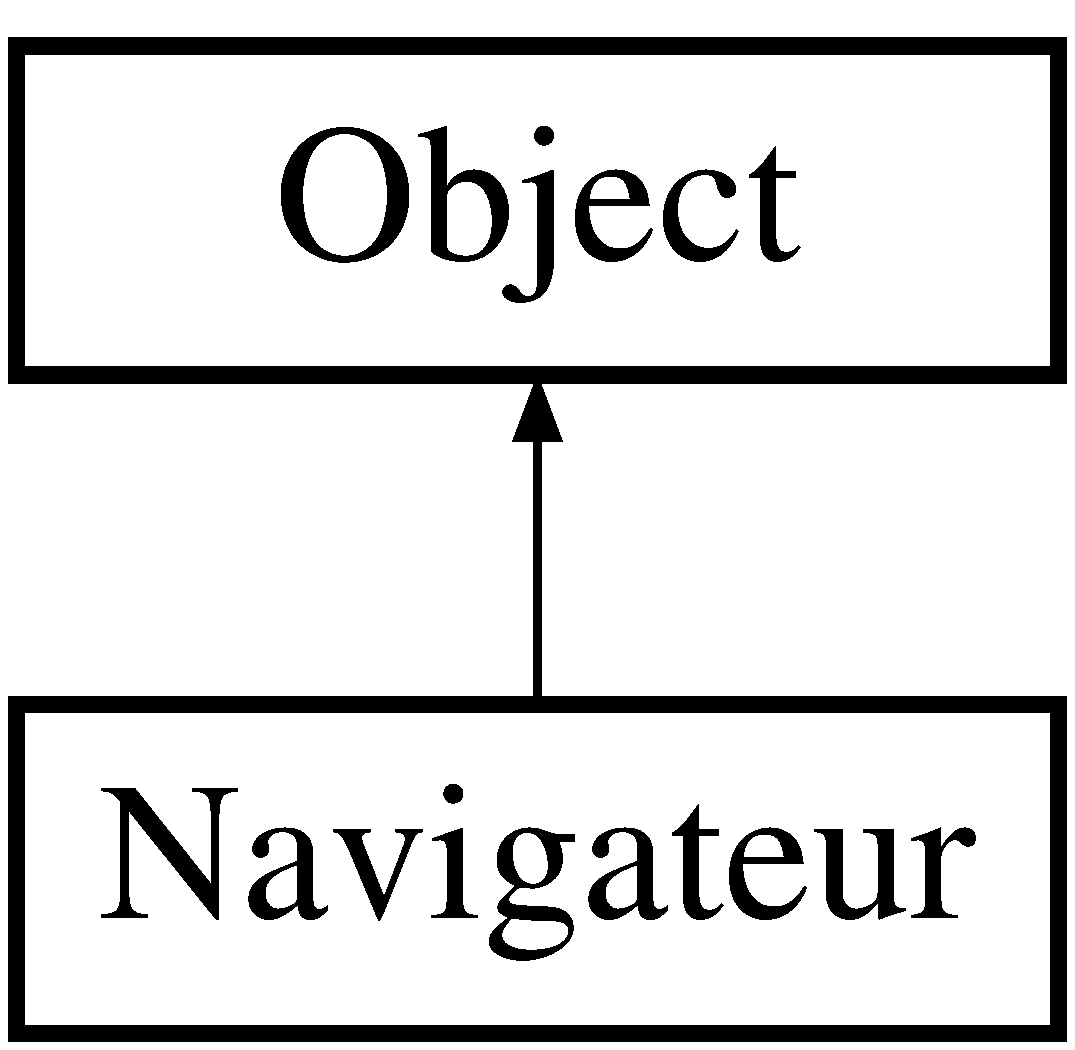
\includegraphics[height=2.000000cm]{class_navigateur}
\end{center}
\end{figure}
\subsection*{Fonctions membres publiques}
\begin{DoxyCompactItemize}
\item 
\hyperlink{class_navigateur_a4a85323eec03cc4c708d6769bc25913f}{Navigateur} ()
\begin{DoxyCompactList}\small\item\em Constructeur. \end{DoxyCompactList}\item 
void \hyperlink{class_navigateur_ad70bb3a8f49254b3e1415b5fabc79473}{deplacement\+Gauche} (const \hyperlink{class_terrain}{Terrain} \&t)
\begin{DoxyCompactList}\small\item\em Deplace le \hyperlink{class_navigateur}{Navigateur} d\textquotesingle{}un cran à gauche. \end{DoxyCompactList}\item 
void \hyperlink{class_navigateur_a1cf57edc86607b309dd2ff77a6ebf535}{deplacement\+Droite} (const \hyperlink{class_terrain}{Terrain} \&t)
\begin{DoxyCompactList}\small\item\em Deplace le \hyperlink{class_navigateur}{Navigateur} d\textquotesingle{}un cran à droite. \end{DoxyCompactList}\item 
void \hyperlink{class_navigateur_a87c978de070d8fb88ea14c4383009246}{deplacement\+Haut} (const \hyperlink{class_terrain}{Terrain} \&t)
\begin{DoxyCompactList}\small\item\em Deplace le \hyperlink{class_navigateur}{Navigateur} d\textquotesingle{}un cran en haut. \end{DoxyCompactList}\item 
void \hyperlink{class_navigateur_a0b8f8dff62930f05df3f8ab758396286}{deplacement\+Bas} (const \hyperlink{class_terrain}{Terrain} \&t)
\begin{DoxyCompactList}\small\item\em Deplace le \hyperlink{class_navigateur}{Navigateur} d\textquotesingle{}un cran en bas. \end{DoxyCompactList}\item 
int \hyperlink{class_navigateur_a02507fc847204a3650378b76072b3e30}{get\+Chance} () const
\begin{DoxyCompactList}\small\item\em Accesseur de la class \hyperlink{class_navigateur}{Navigateur}. \end{DoxyCompactList}\item 
int \hyperlink{class_navigateur_a52606df1f11308074aa64a81cc25e467}{get\+Score} () const
\begin{DoxyCompactList}\small\item\em Accesseur de la class \hyperlink{class_navigateur}{Navigateur}. \end{DoxyCompactList}\item 
int \hyperlink{class_navigateur_a904f67b146dbb561d72cc38ead3d7318}{get\+Niv} () const
\begin{DoxyCompactList}\small\item\em Accesseur de la class \hyperlink{class_navigateur}{Navigateur}. \end{DoxyCompactList}\item 
void \hyperlink{class_navigateur_a4b626cdf47683b637b1e9e000fae467b}{set\+Chance} (int n)
\begin{DoxyCompactList}\small\item\em Mutateur de la class \hyperlink{class_navigateur}{Navigateur}. \end{DoxyCompactList}\item 
void \hyperlink{class_navigateur_a85b21f5d57ed9e03e3276c369eb00fd7}{set\+Score} (int s)
\begin{DoxyCompactList}\small\item\em Mutateur de la class \hyperlink{class_navigateur}{Navigateur}. \end{DoxyCompactList}\item 
void \hyperlink{class_navigateur_af5d5be24410820dfebd15fb5b0966920}{set\+Niv} (int ni)
\begin{DoxyCompactList}\small\item\em Mutateur de la class \hyperlink{class_navigateur}{Navigateur}. \end{DoxyCompactList}\item 
void \hyperlink{class_navigateur_acfd9f284039fa874e7dc146c5cbc9867}{Gestion\+Vie} ()
\begin{DoxyCompactList}\small\item\em Enlève une chance si le navigateur tombe à 0 point de vie et \char`\"{}recommence la partie\char`\"{}, si le navigateur n\textquotesingle{}a plus de vie on sort du programme. \end{DoxyCompactList}\item 
void \hyperlink{class_navigateur_a975f7dc7ac781d977090c75050a1920c}{attaque} (\hyperlink{class_ennemi}{Ennemi} \&p, const \hyperlink{class_terrain}{Terrain} \&t, \hyperlink{class_shoot}{Shoot} \&b)
\begin{DoxyCompactList}\small\item\em Le navigateur tire et augmente le score de 5 si le shoot touche l\textquotesingle{}ennemi, et le niveau de 1 si l\textquotesingle{}ennemi meurt. \end{DoxyCompactList}\item 
bool \hyperlink{class_navigateur_a7d7e08b7a2ace26acdb059af247889e3}{collision} (\hyperlink{class_ennemi}{Ennemi} \&p, const \hyperlink{class_terrain}{Terrain} \&t, \hyperlink{class_shoot}{Shoot} \&b)
\begin{DoxyCompactList}\small\item\em Renvoie true si le shoot du navigateur rencontre la position de l\textquotesingle{}ennemi et inflige des dégats à ce dernier, sinon renvoie false. \end{DoxyCompactList}\item 
void \hyperlink{class_navigateur_a082da7d5d52c149fa234cb856e19c455}{Deplacement\+Shoot} (\hyperlink{class_shoot}{Shoot} \&bn, const \hyperlink{class_terrain}{Terrain} \&t)
\begin{DoxyCompactList}\small\item\em Déplace le shoot du \hyperlink{class_navigateur}{Navigateur} d\textquotesingle{}un cran à gauche si la position qui suit celui-\/ci est libre. \end{DoxyCompactList}\end{DoxyCompactItemize}
\subsection*{Attributs privés}
\begin{DoxyCompactItemize}
\item 
int \hyperlink{class_navigateur_ab6a02c421ddd9d1d5951530b82db6573}{n\+\_\+chance}
\item 
int \hyperlink{class_navigateur_acfbec2e6b65cfe62b591becb70ea0105}{score}
\item 
int \hyperlink{class_navigateur_a1451d9d6397ad3869617876b178324e9}{niv}
\end{DoxyCompactItemize}


\subsection{Description détaillée}
classe utilisée pour la gestion du \hyperlink{class_navigateur}{Navigateur(joueur)}. \hyperlink{class_navigateur}{Navigateur} hérite de la classe \hyperlink{class_object}{Object}. 


\begin{DoxyParams}[1]{Paramètres}
\mbox{\tt in}  & {\em n\+\_\+chance} & Nombre de morts possible du \hyperlink{class_navigateur}{Navigateur} avant défaite. \\
\hline
\mbox{\tt in}  & {\em score} & Score du \hyperlink{class_navigateur}{Navigateur} \\
\hline
\mbox{\tt in}  & {\em niv} & Niveau du \hyperlink{class_navigateur}{Navigateur} \\
\hline
\end{DoxyParams}


\subsection{Documentation des constructeurs et destructeur}
\mbox{\Hypertarget{class_navigateur_a4a85323eec03cc4c708d6769bc25913f}\label{class_navigateur_a4a85323eec03cc4c708d6769bc25913f}} 
\index{Navigateur@{Navigateur}!Navigateur@{Navigateur}}
\index{Navigateur@{Navigateur}!Navigateur@{Navigateur}}
\subsubsection{\texorpdfstring{Navigateur()}{Navigateur()}}
{\footnotesize\ttfamily Navigateur\+::\+Navigateur (\begin{DoxyParamCaption}{ }\end{DoxyParamCaption})}



Constructeur. 

Constructeur par défaut de la classe \hyperlink{class_navigateur}{Navigateur} 

\subsection{Documentation des fonctions membres}
\mbox{\Hypertarget{class_navigateur_a975f7dc7ac781d977090c75050a1920c}\label{class_navigateur_a975f7dc7ac781d977090c75050a1920c}} 
\index{Navigateur@{Navigateur}!attaque@{attaque}}
\index{attaque@{attaque}!Navigateur@{Navigateur}}
\subsubsection{\texorpdfstring{attaque()}{attaque()}}
{\footnotesize\ttfamily void Navigateur\+::attaque (\begin{DoxyParamCaption}\item[{\hyperlink{class_ennemi}{Ennemi} \&}]{p,  }\item[{const \hyperlink{class_terrain}{Terrain} \&}]{t,  }\item[{\hyperlink{class_shoot}{Shoot} \&}]{b }\end{DoxyParamCaption})}



Le navigateur tire et augmente le score de 5 si le shoot touche l\textquotesingle{}ennemi, et le niveau de 1 si l\textquotesingle{}ennemi meurt. 


\begin{DoxyParams}{Paramètres}
{\em p} & \+: référence sur \hyperlink{class_ennemi}{Ennemi} \\
\hline
{\em t} & \+: de type \hyperlink{class_terrain}{Terrain} \\
\hline
{\em b} & \+: de type \hyperlink{class_shoot}{Shoot} \\
\hline
\end{DoxyParams}
\mbox{\Hypertarget{class_navigateur_a7d7e08b7a2ace26acdb059af247889e3}\label{class_navigateur_a7d7e08b7a2ace26acdb059af247889e3}} 
\index{Navigateur@{Navigateur}!collision@{collision}}
\index{collision@{collision}!Navigateur@{Navigateur}}
\subsubsection{\texorpdfstring{collision()}{collision()}}
{\footnotesize\ttfamily bool Navigateur\+::collision (\begin{DoxyParamCaption}\item[{\hyperlink{class_ennemi}{Ennemi} \&}]{p,  }\item[{const \hyperlink{class_terrain}{Terrain} \&}]{t,  }\item[{\hyperlink{class_shoot}{Shoot} \&}]{b }\end{DoxyParamCaption})}



Renvoie true si le shoot du navigateur rencontre la position de l\textquotesingle{}ennemi et inflige des dégats à ce dernier, sinon renvoie false. 


\begin{DoxyParams}{Paramètres}
{\em p} & \+: référence sur \hyperlink{class_ennemi}{Ennemi} \\
\hline
{\em t} & \+: de type \hyperlink{class_terrain}{Terrain} \\
\hline
{\em b} & \+: de type \hyperlink{class_shoot}{Shoot} \\
\hline
\end{DoxyParams}
\mbox{\Hypertarget{class_navigateur_a0b8f8dff62930f05df3f8ab758396286}\label{class_navigateur_a0b8f8dff62930f05df3f8ab758396286}} 
\index{Navigateur@{Navigateur}!deplacement\+Bas@{deplacement\+Bas}}
\index{deplacement\+Bas@{deplacement\+Bas}!Navigateur@{Navigateur}}
\subsubsection{\texorpdfstring{deplacement\+Bas()}{deplacementBas()}}
{\footnotesize\ttfamily void Navigateur\+::deplacement\+Bas (\begin{DoxyParamCaption}\item[{const \hyperlink{class_terrain}{Terrain} \&}]{t }\end{DoxyParamCaption})}



Deplace le \hyperlink{class_navigateur}{Navigateur} d\textquotesingle{}un cran en bas. 


\begin{DoxyParams}{Paramètres}
{\em t} & \+: de type \hyperlink{class_terrain}{Terrain} \\
\hline
\end{DoxyParams}
\mbox{\Hypertarget{class_navigateur_a1cf57edc86607b309dd2ff77a6ebf535}\label{class_navigateur_a1cf57edc86607b309dd2ff77a6ebf535}} 
\index{Navigateur@{Navigateur}!deplacement\+Droite@{deplacement\+Droite}}
\index{deplacement\+Droite@{deplacement\+Droite}!Navigateur@{Navigateur}}
\subsubsection{\texorpdfstring{deplacement\+Droite()}{deplacementDroite()}}
{\footnotesize\ttfamily void Navigateur\+::deplacement\+Droite (\begin{DoxyParamCaption}\item[{const \hyperlink{class_terrain}{Terrain} \&}]{t }\end{DoxyParamCaption})}



Deplace le \hyperlink{class_navigateur}{Navigateur} d\textquotesingle{}un cran à droite. 


\begin{DoxyParams}{Paramètres}
{\em t} & \+: de type \hyperlink{class_terrain}{Terrain} \\
\hline
\end{DoxyParams}
\mbox{\Hypertarget{class_navigateur_ad70bb3a8f49254b3e1415b5fabc79473}\label{class_navigateur_ad70bb3a8f49254b3e1415b5fabc79473}} 
\index{Navigateur@{Navigateur}!deplacement\+Gauche@{deplacement\+Gauche}}
\index{deplacement\+Gauche@{deplacement\+Gauche}!Navigateur@{Navigateur}}
\subsubsection{\texorpdfstring{deplacement\+Gauche()}{deplacementGauche()}}
{\footnotesize\ttfamily void Navigateur\+::deplacement\+Gauche (\begin{DoxyParamCaption}\item[{const \hyperlink{class_terrain}{Terrain} \&}]{t }\end{DoxyParamCaption})}



Deplace le \hyperlink{class_navigateur}{Navigateur} d\textquotesingle{}un cran à gauche. 


\begin{DoxyParams}{Paramètres}
{\em t} & \+: de type \hyperlink{class_terrain}{Terrain} \\
\hline
\end{DoxyParams}
\mbox{\Hypertarget{class_navigateur_a87c978de070d8fb88ea14c4383009246}\label{class_navigateur_a87c978de070d8fb88ea14c4383009246}} 
\index{Navigateur@{Navigateur}!deplacement\+Haut@{deplacement\+Haut}}
\index{deplacement\+Haut@{deplacement\+Haut}!Navigateur@{Navigateur}}
\subsubsection{\texorpdfstring{deplacement\+Haut()}{deplacementHaut()}}
{\footnotesize\ttfamily void Navigateur\+::deplacement\+Haut (\begin{DoxyParamCaption}\item[{const \hyperlink{class_terrain}{Terrain} \&}]{t }\end{DoxyParamCaption})}



Deplace le \hyperlink{class_navigateur}{Navigateur} d\textquotesingle{}un cran en haut. 


\begin{DoxyParams}{Paramètres}
{\em t} & \+: de type \hyperlink{class_terrain}{Terrain} \\
\hline
\end{DoxyParams}
\mbox{\Hypertarget{class_navigateur_a082da7d5d52c149fa234cb856e19c455}\label{class_navigateur_a082da7d5d52c149fa234cb856e19c455}} 
\index{Navigateur@{Navigateur}!Deplacement\+Shoot@{Deplacement\+Shoot}}
\index{Deplacement\+Shoot@{Deplacement\+Shoot}!Navigateur@{Navigateur}}
\subsubsection{\texorpdfstring{Deplacement\+Shoot()}{DeplacementShoot()}}
{\footnotesize\ttfamily void Navigateur\+::\+Deplacement\+Shoot (\begin{DoxyParamCaption}\item[{\hyperlink{class_shoot}{Shoot} \&}]{bn,  }\item[{const \hyperlink{class_terrain}{Terrain} \&}]{t }\end{DoxyParamCaption})}



Déplace le shoot du \hyperlink{class_navigateur}{Navigateur} d\textquotesingle{}un cran à gauche si la position qui suit celui-\/ci est libre. 


\begin{DoxyParams}{Paramètres}
{\em t} & \+: de type \hyperlink{class_terrain}{Terrain} \\
\hline
{\em bn} & \+: de type \hyperlink{class_shoot}{Shoot} \\
\hline
\end{DoxyParams}
\mbox{\Hypertarget{class_navigateur_acfd9f284039fa874e7dc146c5cbc9867}\label{class_navigateur_acfd9f284039fa874e7dc146c5cbc9867}} 
\index{Navigateur@{Navigateur}!Gestion\+Vie@{Gestion\+Vie}}
\index{Gestion\+Vie@{Gestion\+Vie}!Navigateur@{Navigateur}}
\subsubsection{\texorpdfstring{Gestion\+Vie()}{GestionVie()}}
{\footnotesize\ttfamily void Navigateur\+::\+Gestion\+Vie (\begin{DoxyParamCaption}{ }\end{DoxyParamCaption})}



Enlève une chance si le navigateur tombe à 0 point de vie et \char`\"{}recommence la partie\char`\"{}, si le navigateur n\textquotesingle{}a plus de vie on sort du programme. 

\mbox{\Hypertarget{class_navigateur_a02507fc847204a3650378b76072b3e30}\label{class_navigateur_a02507fc847204a3650378b76072b3e30}} 
\index{Navigateur@{Navigateur}!get\+Chance@{get\+Chance}}
\index{get\+Chance@{get\+Chance}!Navigateur@{Navigateur}}
\subsubsection{\texorpdfstring{get\+Chance()}{getChance()}}
{\footnotesize\ttfamily int Navigateur\+::get\+Chance (\begin{DoxyParamCaption}{ }\end{DoxyParamCaption}) const}



Accesseur de la class \hyperlink{class_navigateur}{Navigateur}. 

int \hyperlink{class_navigateur_a02507fc847204a3650378b76072b3e30}{get\+Chance() const}; \mbox{\Hypertarget{class_navigateur_a904f67b146dbb561d72cc38ead3d7318}\label{class_navigateur_a904f67b146dbb561d72cc38ead3d7318}} 
\index{Navigateur@{Navigateur}!get\+Niv@{get\+Niv}}
\index{get\+Niv@{get\+Niv}!Navigateur@{Navigateur}}
\subsubsection{\texorpdfstring{get\+Niv()}{getNiv()}}
{\footnotesize\ttfamily int Navigateur\+::get\+Niv (\begin{DoxyParamCaption}{ }\end{DoxyParamCaption}) const}



Accesseur de la class \hyperlink{class_navigateur}{Navigateur}. 

int \hyperlink{class_navigateur_a904f67b146dbb561d72cc38ead3d7318}{get\+Niv() const}; \mbox{\Hypertarget{class_navigateur_a52606df1f11308074aa64a81cc25e467}\label{class_navigateur_a52606df1f11308074aa64a81cc25e467}} 
\index{Navigateur@{Navigateur}!get\+Score@{get\+Score}}
\index{get\+Score@{get\+Score}!Navigateur@{Navigateur}}
\subsubsection{\texorpdfstring{get\+Score()}{getScore()}}
{\footnotesize\ttfamily int Navigateur\+::get\+Score (\begin{DoxyParamCaption}{ }\end{DoxyParamCaption}) const}



Accesseur de la class \hyperlink{class_navigateur}{Navigateur}. 

int \hyperlink{class_navigateur_a52606df1f11308074aa64a81cc25e467}{get\+Score() const}; \mbox{\Hypertarget{class_navigateur_a4b626cdf47683b637b1e9e000fae467b}\label{class_navigateur_a4b626cdf47683b637b1e9e000fae467b}} 
\index{Navigateur@{Navigateur}!set\+Chance@{set\+Chance}}
\index{set\+Chance@{set\+Chance}!Navigateur@{Navigateur}}
\subsubsection{\texorpdfstring{set\+Chance()}{setChance()}}
{\footnotesize\ttfamily void Navigateur\+::set\+Chance (\begin{DoxyParamCaption}\item[{int}]{n }\end{DoxyParamCaption})}



Mutateur de la class \hyperlink{class_navigateur}{Navigateur}. 

void \hyperlink{class_navigateur_a4b626cdf47683b637b1e9e000fae467b}{set\+Chance(int n)}; \mbox{\Hypertarget{class_navigateur_af5d5be24410820dfebd15fb5b0966920}\label{class_navigateur_af5d5be24410820dfebd15fb5b0966920}} 
\index{Navigateur@{Navigateur}!set\+Niv@{set\+Niv}}
\index{set\+Niv@{set\+Niv}!Navigateur@{Navigateur}}
\subsubsection{\texorpdfstring{set\+Niv()}{setNiv()}}
{\footnotesize\ttfamily void Navigateur\+::set\+Niv (\begin{DoxyParamCaption}\item[{int}]{ni }\end{DoxyParamCaption})}



Mutateur de la class \hyperlink{class_navigateur}{Navigateur}. 

void \hyperlink{class_navigateur_af5d5be24410820dfebd15fb5b0966920}{set\+Niv(int ni)}; \mbox{\Hypertarget{class_navigateur_a85b21f5d57ed9e03e3276c369eb00fd7}\label{class_navigateur_a85b21f5d57ed9e03e3276c369eb00fd7}} 
\index{Navigateur@{Navigateur}!set\+Score@{set\+Score}}
\index{set\+Score@{set\+Score}!Navigateur@{Navigateur}}
\subsubsection{\texorpdfstring{set\+Score()}{setScore()}}
{\footnotesize\ttfamily void Navigateur\+::set\+Score (\begin{DoxyParamCaption}\item[{int}]{s }\end{DoxyParamCaption})}



Mutateur de la class \hyperlink{class_navigateur}{Navigateur}. 

void \hyperlink{class_navigateur_a85b21f5d57ed9e03e3276c369eb00fd7}{set\+Score(int s)}; 

\subsection{Documentation des données membres}
\mbox{\Hypertarget{class_navigateur_ab6a02c421ddd9d1d5951530b82db6573}\label{class_navigateur_ab6a02c421ddd9d1d5951530b82db6573}} 
\index{Navigateur@{Navigateur}!n\+\_\+chance@{n\+\_\+chance}}
\index{n\+\_\+chance@{n\+\_\+chance}!Navigateur@{Navigateur}}
\subsubsection{\texorpdfstring{n\+\_\+chance}{n\_chance}}
{\footnotesize\ttfamily int Navigateur\+::n\+\_\+chance\hspace{0.3cm}{\ttfamily [private]}}

\mbox{\Hypertarget{class_navigateur_a1451d9d6397ad3869617876b178324e9}\label{class_navigateur_a1451d9d6397ad3869617876b178324e9}} 
\index{Navigateur@{Navigateur}!niv@{niv}}
\index{niv@{niv}!Navigateur@{Navigateur}}
\subsubsection{\texorpdfstring{niv}{niv}}
{\footnotesize\ttfamily int Navigateur\+::niv\hspace{0.3cm}{\ttfamily [private]}}

\mbox{\Hypertarget{class_navigateur_acfbec2e6b65cfe62b591becb70ea0105}\label{class_navigateur_acfbec2e6b65cfe62b591becb70ea0105}} 
\index{Navigateur@{Navigateur}!score@{score}}
\index{score@{score}!Navigateur@{Navigateur}}
\subsubsection{\texorpdfstring{score}{score}}
{\footnotesize\ttfamily int Navigateur\+::score\hspace{0.3cm}{\ttfamily [private]}}



La documentation de cette classe a été générée à partir des fichiers suivants \+:\begin{DoxyCompactItemize}
\item 
C\+:/\+Users/\+Ragnar\+L/\+Documents/p1408299-\/p1309837/\+Revenges\+Island/src/core/\hyperlink{_navigateur_8h}{Navigateur.\+h}\item 
C\+:/\+Users/\+Ragnar\+L/\+Documents/p1408299-\/p1309837/\+Revenges\+Island/src/core/\hyperlink{_navigateur_8cpp}{Navigateur.\+cpp}\end{DoxyCompactItemize}

\hypertarget{class_object}{}\section{Référence de la classe Object}
\label{class_object}\index{Object@{Object}}


classe utilisée pour la gestion des Objets.  




{\ttfamily \#include $<$Object.\+h$>$}

Graphe d\textquotesingle{}héritage de Object\+:\begin{figure}[H]
\begin{center}
\leavevmode
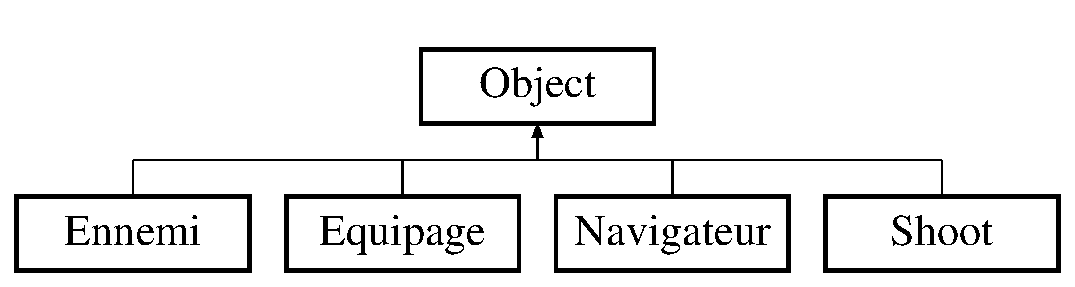
\includegraphics[height=2.000000cm]{class_object}
\end{center}
\end{figure}
\subsection*{Fonctions membres publiques}
\begin{DoxyCompactItemize}
\item 
\hyperlink{class_object_a40860402e64d8008fb42329df7097cdb}{Object} ()
\begin{DoxyCompactList}\small\item\em Constructeur. \end{DoxyCompactList}\item 
\hyperlink{class_object_abdc77f1bc660f185ecf2fc1a628ea6eb}{Object} (int x, int y)
\begin{DoxyCompactList}\small\item\em Constructeur par copie. \end{DoxyCompactList}\item 
int \hyperlink{class_object_ad7dcd5f1f45ce373c6e57bae5d1aebec}{get\+Pos\+\_\+x} () const
\begin{DoxyCompactList}\small\item\em Accesseur de la class \hyperlink{class_object}{Object}. \end{DoxyCompactList}\item 
int \hyperlink{class_object_a74b891ac92f211e8d8f9fd09d7822ec4}{get\+Pos\+\_\+y} () const
\begin{DoxyCompactList}\small\item\em Accesseur de la class \hyperlink{class_object}{Object}. \end{DoxyCompactList}\item 
int \hyperlink{class_object_ac2053fa5af98fc92a4c990946a926aa5}{get\+Dir} () const
\begin{DoxyCompactList}\small\item\em Accesseur de la class \hyperlink{class_object}{Object}. \end{DoxyCompactList}\item 
int \hyperlink{class_object_a334099b7bd5ecf8515a1e8f3d96ebba9}{get\+Vie} () const
\begin{DoxyCompactList}\small\item\em Accesseur de la class \hyperlink{class_object}{Object}. \end{DoxyCompactList}\item 
void \hyperlink{class_object_a65c8e1794d02320269340d22084d0807}{set\+Pos\+\_\+x} (int x)
\begin{DoxyCompactList}\small\item\em Mutateur de la class \hyperlink{class_object}{Object}. \end{DoxyCompactList}\item 
void \hyperlink{class_object_a35340b9a66cc2d561ad370783c41fcac}{set\+Pos\+\_\+y} (int y)
\begin{DoxyCompactList}\small\item\em Mutateur de la class \hyperlink{class_object}{Object}. \end{DoxyCompactList}\item 
void \hyperlink{class_object_a6d72ba9034f1ea3a0866574705e938d3}{set\+Dir} (int di)
\begin{DoxyCompactList}\small\item\em Mutateur de la class \hyperlink{class_object}{Object}. \end{DoxyCompactList}\item 
void \hyperlink{class_object_ac0880db52bcbcd3022278d62956d666e}{set\+Vie} (int v)
\begin{DoxyCompactList}\small\item\em Mutateur de la class \hyperlink{class_object}{Object}. \end{DoxyCompactList}\item 
void \hyperlink{class_object_a9e7f78b7cc24ebe4d11e8ce7b86c1d49}{set\+Position} (int x, int y)
\begin{DoxyCompactList}\small\item\em Mutateur de la class \hyperlink{class_object}{Object}. \end{DoxyCompactList}\item 
void \hyperlink{class_object_a98f9245de6001ab13932531b047ba595}{recevoir\+Degats} (int nb\+Degats)
\begin{DoxyCompactList}\small\item\em Enlève des points de vie à l\textquotesingle{}\hyperlink{class_objet}{Objet}. \end{DoxyCompactList}\item 
bool \hyperlink{class_object_ae013d3c24ca77287536bfc594f763b60}{est\+Vivant} ()
\begin{DoxyCompactList}\small\item\em Renvoit true si l\textquotesingle{}\hyperlink{class_objet}{Objet} à encore des points de vie et false sinon. \end{DoxyCompactList}\end{DoxyCompactItemize}
\subsection*{Attributs privés}
\begin{DoxyCompactItemize}
\item 
int \hyperlink{class_object_a2fc9911a2ee453f97ccfad331dc29e3a}{pos\+\_\+x}
\item 
int \hyperlink{class_object_a5acac61f66b23f32ad2ed7aa2e93c307}{pos\+\_\+y}
\item 
int \hyperlink{class_object_a1267bc5eb5865f7ad9de7d822483c0e0}{dir}
\item 
int \hyperlink{class_object_a1710b8b8e0d814406f84ca905d411e69}{p\+\_\+vie}
\end{DoxyCompactItemize}


\subsection{Description détaillée}
classe utilisée pour la gestion des Objets. 


\begin{DoxyParams}[1]{Paramètres}
\mbox{\tt in}  & {\em pos\+\_\+x} & \+: entier définit la position en abscisse de l\textquotesingle{}objet \\
\hline
\mbox{\tt in}  & {\em pos\+\_\+y} & \+: entier définit la position en ordonnée de l\textquotesingle{}objet \\
\hline
\mbox{\tt in}  & {\em dir} & \+: entier définit la direction de déplacement futur de l\textquotesingle{}objet \\
\hline
\mbox{\tt in}  & {\em p\+\_\+vie} & \+: entier définit les points de vie de l\textquotesingle{}objet \\
\hline
\end{DoxyParams}


\subsection{Documentation des constructeurs et destructeur}
\mbox{\Hypertarget{class_object_a40860402e64d8008fb42329df7097cdb}\label{class_object_a40860402e64d8008fb42329df7097cdb}} 
\index{Object@{Object}!Object@{Object}}
\index{Object@{Object}!Object@{Object}}
\subsubsection{\texorpdfstring{Object()}{Object()}\hspace{0.1cm}{\footnotesize\ttfamily [1/2]}}
{\footnotesize\ttfamily Object\+::\+Object (\begin{DoxyParamCaption}{ }\end{DoxyParamCaption})}



Constructeur. 

Constructeur par défaut de la classe \hyperlink{class_object}{Object} \mbox{\Hypertarget{class_object_abdc77f1bc660f185ecf2fc1a628ea6eb}\label{class_object_abdc77f1bc660f185ecf2fc1a628ea6eb}} 
\index{Object@{Object}!Object@{Object}}
\index{Object@{Object}!Object@{Object}}
\subsubsection{\texorpdfstring{Object()}{Object()}\hspace{0.1cm}{\footnotesize\ttfamily [2/2]}}
{\footnotesize\ttfamily Object\+::\+Object (\begin{DoxyParamCaption}\item[{int}]{x,  }\item[{int}]{y }\end{DoxyParamCaption})}



Constructeur par copie. 

Constructeur par copie de la classe \hyperlink{class_object}{Object}


\begin{DoxyParams}{Paramètres}
{\em x} & \+: entier correspondant à pos\+\_\+x \\
\hline
{\em y} & \+: entier correspondant à pos\+\_\+y \\
\hline
\end{DoxyParams}


\subsection{Documentation des fonctions membres}
\mbox{\Hypertarget{class_object_ae013d3c24ca77287536bfc594f763b60}\label{class_object_ae013d3c24ca77287536bfc594f763b60}} 
\index{Object@{Object}!est\+Vivant@{est\+Vivant}}
\index{est\+Vivant@{est\+Vivant}!Object@{Object}}
\subsubsection{\texorpdfstring{est\+Vivant()}{estVivant()}}
{\footnotesize\ttfamily bool Object\+::est\+Vivant (\begin{DoxyParamCaption}{ }\end{DoxyParamCaption})}



Renvoit true si l\textquotesingle{}\hyperlink{class_objet}{Objet} à encore des points de vie et false sinon. 

\mbox{\Hypertarget{class_object_ac2053fa5af98fc92a4c990946a926aa5}\label{class_object_ac2053fa5af98fc92a4c990946a926aa5}} 
\index{Object@{Object}!get\+Dir@{get\+Dir}}
\index{get\+Dir@{get\+Dir}!Object@{Object}}
\subsubsection{\texorpdfstring{get\+Dir()}{getDir()}}
{\footnotesize\ttfamily int Object\+::get\+Dir (\begin{DoxyParamCaption}{ }\end{DoxyParamCaption}) const}



Accesseur de la class \hyperlink{class_object}{Object}. 

int \hyperlink{class_object_ac2053fa5af98fc92a4c990946a926aa5}{get\+Dir() const}; \mbox{\Hypertarget{class_object_ad7dcd5f1f45ce373c6e57bae5d1aebec}\label{class_object_ad7dcd5f1f45ce373c6e57bae5d1aebec}} 
\index{Object@{Object}!get\+Pos\+\_\+x@{get\+Pos\+\_\+x}}
\index{get\+Pos\+\_\+x@{get\+Pos\+\_\+x}!Object@{Object}}
\subsubsection{\texorpdfstring{get\+Pos\+\_\+x()}{getPos\_x()}}
{\footnotesize\ttfamily int Object\+::get\+Pos\+\_\+x (\begin{DoxyParamCaption}{ }\end{DoxyParamCaption}) const}



Accesseur de la class \hyperlink{class_object}{Object}. 

int \hyperlink{class_object_ad7dcd5f1f45ce373c6e57bae5d1aebec}{get\+Pos\+\_\+x() const}; \mbox{\Hypertarget{class_object_a74b891ac92f211e8d8f9fd09d7822ec4}\label{class_object_a74b891ac92f211e8d8f9fd09d7822ec4}} 
\index{Object@{Object}!get\+Pos\+\_\+y@{get\+Pos\+\_\+y}}
\index{get\+Pos\+\_\+y@{get\+Pos\+\_\+y}!Object@{Object}}
\subsubsection{\texorpdfstring{get\+Pos\+\_\+y()}{getPos\_y()}}
{\footnotesize\ttfamily int Object\+::get\+Pos\+\_\+y (\begin{DoxyParamCaption}{ }\end{DoxyParamCaption}) const}



Accesseur de la class \hyperlink{class_object}{Object}. 

int \hyperlink{class_object_a74b891ac92f211e8d8f9fd09d7822ec4}{get\+Pos\+\_\+y() const}; \mbox{\Hypertarget{class_object_a334099b7bd5ecf8515a1e8f3d96ebba9}\label{class_object_a334099b7bd5ecf8515a1e8f3d96ebba9}} 
\index{Object@{Object}!get\+Vie@{get\+Vie}}
\index{get\+Vie@{get\+Vie}!Object@{Object}}
\subsubsection{\texorpdfstring{get\+Vie()}{getVie()}}
{\footnotesize\ttfamily int Object\+::get\+Vie (\begin{DoxyParamCaption}{ }\end{DoxyParamCaption}) const}



Accesseur de la class \hyperlink{class_object}{Object}. 

int \hyperlink{class_object_a334099b7bd5ecf8515a1e8f3d96ebba9}{get\+Vie() const}; \mbox{\Hypertarget{class_object_a98f9245de6001ab13932531b047ba595}\label{class_object_a98f9245de6001ab13932531b047ba595}} 
\index{Object@{Object}!recevoir\+Degats@{recevoir\+Degats}}
\index{recevoir\+Degats@{recevoir\+Degats}!Object@{Object}}
\subsubsection{\texorpdfstring{recevoir\+Degats()}{recevoirDegats()}}
{\footnotesize\ttfamily void Object\+::recevoir\+Degats (\begin{DoxyParamCaption}\item[{int}]{nb\+Degats }\end{DoxyParamCaption})}



Enlève des points de vie à l\textquotesingle{}\hyperlink{class_objet}{Objet}. 


\begin{DoxyParams}{Paramètres}
{\em nb\+Degats} & \+: entier définit le nombre de points de vie à enlever \\
\hline
\end{DoxyParams}
\mbox{\Hypertarget{class_object_a6d72ba9034f1ea3a0866574705e938d3}\label{class_object_a6d72ba9034f1ea3a0866574705e938d3}} 
\index{Object@{Object}!set\+Dir@{set\+Dir}}
\index{set\+Dir@{set\+Dir}!Object@{Object}}
\subsubsection{\texorpdfstring{set\+Dir()}{setDir()}}
{\footnotesize\ttfamily void Object\+::set\+Dir (\begin{DoxyParamCaption}\item[{int}]{di }\end{DoxyParamCaption})}



Mutateur de la class \hyperlink{class_object}{Object}. 

void \hyperlink{class_object_a6d72ba9034f1ea3a0866574705e938d3}{set\+Dir(int di)}; \mbox{\Hypertarget{class_object_a65c8e1794d02320269340d22084d0807}\label{class_object_a65c8e1794d02320269340d22084d0807}} 
\index{Object@{Object}!set\+Pos\+\_\+x@{set\+Pos\+\_\+x}}
\index{set\+Pos\+\_\+x@{set\+Pos\+\_\+x}!Object@{Object}}
\subsubsection{\texorpdfstring{set\+Pos\+\_\+x()}{setPos\_x()}}
{\footnotesize\ttfamily void Object\+::set\+Pos\+\_\+x (\begin{DoxyParamCaption}\item[{int}]{x }\end{DoxyParamCaption})}



Mutateur de la class \hyperlink{class_object}{Object}. 

void \hyperlink{class_object_a65c8e1794d02320269340d22084d0807}{set\+Pos\+\_\+x(int x)}; \mbox{\Hypertarget{class_object_a35340b9a66cc2d561ad370783c41fcac}\label{class_object_a35340b9a66cc2d561ad370783c41fcac}} 
\index{Object@{Object}!set\+Pos\+\_\+y@{set\+Pos\+\_\+y}}
\index{set\+Pos\+\_\+y@{set\+Pos\+\_\+y}!Object@{Object}}
\subsubsection{\texorpdfstring{set\+Pos\+\_\+y()}{setPos\_y()}}
{\footnotesize\ttfamily void Object\+::set\+Pos\+\_\+y (\begin{DoxyParamCaption}\item[{int}]{y }\end{DoxyParamCaption})}



Mutateur de la class \hyperlink{class_object}{Object}. 

void \hyperlink{class_object_a35340b9a66cc2d561ad370783c41fcac}{set\+Pos\+\_\+y(int x)}; \mbox{\Hypertarget{class_object_a9e7f78b7cc24ebe4d11e8ce7b86c1d49}\label{class_object_a9e7f78b7cc24ebe4d11e8ce7b86c1d49}} 
\index{Object@{Object}!set\+Position@{set\+Position}}
\index{set\+Position@{set\+Position}!Object@{Object}}
\subsubsection{\texorpdfstring{set\+Position()}{setPosition()}}
{\footnotesize\ttfamily void Object\+::set\+Position (\begin{DoxyParamCaption}\item[{int}]{x,  }\item[{int}]{y }\end{DoxyParamCaption})}



Mutateur de la class \hyperlink{class_object}{Object}. 

void \hyperlink{class_object_a9e7f78b7cc24ebe4d11e8ce7b86c1d49}{set\+Position(int x, int y)}; \mbox{\Hypertarget{class_object_ac0880db52bcbcd3022278d62956d666e}\label{class_object_ac0880db52bcbcd3022278d62956d666e}} 
\index{Object@{Object}!set\+Vie@{set\+Vie}}
\index{set\+Vie@{set\+Vie}!Object@{Object}}
\subsubsection{\texorpdfstring{set\+Vie()}{setVie()}}
{\footnotesize\ttfamily void Object\+::set\+Vie (\begin{DoxyParamCaption}\item[{int}]{v }\end{DoxyParamCaption})}



Mutateur de la class \hyperlink{class_object}{Object}. 

void \hyperlink{class_object_ac0880db52bcbcd3022278d62956d666e}{set\+Vie(int v)}; 

\subsection{Documentation des données membres}
\mbox{\Hypertarget{class_object_a1267bc5eb5865f7ad9de7d822483c0e0}\label{class_object_a1267bc5eb5865f7ad9de7d822483c0e0}} 
\index{Object@{Object}!dir@{dir}}
\index{dir@{dir}!Object@{Object}}
\subsubsection{\texorpdfstring{dir}{dir}}
{\footnotesize\ttfamily int Object\+::dir\hspace{0.3cm}{\ttfamily [private]}}

\mbox{\Hypertarget{class_object_a1710b8b8e0d814406f84ca905d411e69}\label{class_object_a1710b8b8e0d814406f84ca905d411e69}} 
\index{Object@{Object}!p\+\_\+vie@{p\+\_\+vie}}
\index{p\+\_\+vie@{p\+\_\+vie}!Object@{Object}}
\subsubsection{\texorpdfstring{p\+\_\+vie}{p\_vie}}
{\footnotesize\ttfamily int Object\+::p\+\_\+vie\hspace{0.3cm}{\ttfamily [private]}}

\mbox{\Hypertarget{class_object_a2fc9911a2ee453f97ccfad331dc29e3a}\label{class_object_a2fc9911a2ee453f97ccfad331dc29e3a}} 
\index{Object@{Object}!pos\+\_\+x@{pos\+\_\+x}}
\index{pos\+\_\+x@{pos\+\_\+x}!Object@{Object}}
\subsubsection{\texorpdfstring{pos\+\_\+x}{pos\_x}}
{\footnotesize\ttfamily int Object\+::pos\+\_\+x\hspace{0.3cm}{\ttfamily [private]}}

\mbox{\Hypertarget{class_object_a5acac61f66b23f32ad2ed7aa2e93c307}\label{class_object_a5acac61f66b23f32ad2ed7aa2e93c307}} 
\index{Object@{Object}!pos\+\_\+y@{pos\+\_\+y}}
\index{pos\+\_\+y@{pos\+\_\+y}!Object@{Object}}
\subsubsection{\texorpdfstring{pos\+\_\+y}{pos\_y}}
{\footnotesize\ttfamily int Object\+::pos\+\_\+y\hspace{0.3cm}{\ttfamily [private]}}



La documentation de cette classe a été générée à partir des fichiers suivants \+:\begin{DoxyCompactItemize}
\item 
C\+:/\+Users/\+Ragnar\+L/\+Documents/p1408299-\/p1309837/\+Revenges\+Island/src/core/\hyperlink{_object_8h}{Object.\+h}\item 
C\+:/\+Users/\+Ragnar\+L/\+Documents/p1408299-\/p1309837/\+Revenges\+Island/src/core/\hyperlink{_object_8cpp}{Object.\+cpp}\end{DoxyCompactItemize}

\hypertarget{class_objet}{}\section{Référence de la classe Objet}
\label{class_objet}\index{Objet@{Objet}}


{\ttfamily \#include $<$Objet.\+h$>$}

Graphe d\textquotesingle{}héritage de Objet\+:\begin{figure}[H]
\begin{center}
\leavevmode
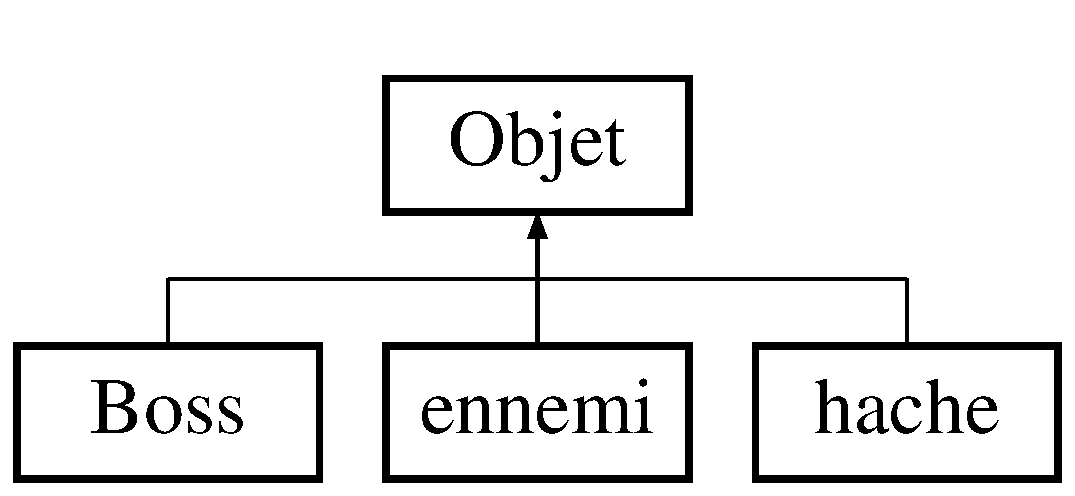
\includegraphics[height=2.000000cm]{class_objet}
\end{center}
\end{figure}
\subsection*{Fonctions membres publiques}
\begin{DoxyCompactItemize}
\item 
\hyperlink{class_objet_aefdd826d50085897e4894ffef4597d04}{Objet} ()
\item 
virtual \hyperlink{class_objet_a77a195bb1452ef4221b5080632cd7757}{$\sim$\+Objet} ()
\item 
void \hyperlink{class_objet_ad4b867d62bf9b79a23d6017cc36b6641}{parametres} (\hyperlink{class_animation}{Animation} \&a, float X, float Y, float Angle=0, int radius=1)
\item 
virtual void \hyperlink{class_objet_a684611b20eb6e6df5e4743dd3e42385a}{update} ()
\item 
void \hyperlink{class_objet_a9d1d8178549d070d7c40635efae24b5e}{draw} (sf\+::\+Render\+Window \&win)
\end{DoxyCompactItemize}
\subsection*{Attributs publics}
\begin{DoxyCompactItemize}
\item 
float \hyperlink{class_objet_a2c73c2c45d5339df8228966b655351de}{x}
\item 
float \hyperlink{class_objet_a875f758fbf6434825b3acdc011b362a2}{y}
\item 
float \hyperlink{class_objet_ae31175118003ae9a862c9ce10f853045}{dx}
\item 
float \hyperlink{class_objet_a6e0d923cb4450478ed31e94ee7f5a531}{dy}
\item 
float \hyperlink{class_objet_ac931833c077df49ec3f909aba38e0121}{R}
\item 
float \hyperlink{class_objet_a1e3e095030fbc53562c5561cabd2e800}{angle}
\item 
bool \hyperlink{class_objet_a50498a805e7a5db752bf5bfd9fbb7b5b}{vie}
\item 
std\+::string \hyperlink{class_objet_aec3ba4223b80d485e9c8c72b17d53b3a}{nom}
\item 
\hyperlink{class_animation}{Animation} \hyperlink{class_objet_a4d1cd0327bccc4022d7b9bbba2c041b5}{anim}
\end{DoxyCompactItemize}


\subsection{Documentation des constructeurs et destructeur}
\mbox{\Hypertarget{class_objet_aefdd826d50085897e4894ffef4597d04}\label{class_objet_aefdd826d50085897e4894ffef4597d04}} 
\index{Objet@{Objet}!Objet@{Objet}}
\index{Objet@{Objet}!Objet@{Objet}}
\subsubsection{\texorpdfstring{Objet()}{Objet()}}
{\footnotesize\ttfamily Objet\+::\+Objet (\begin{DoxyParamCaption}{ }\end{DoxyParamCaption})\hspace{0.3cm}{\ttfamily [inline]}}

\mbox{\Hypertarget{class_objet_a77a195bb1452ef4221b5080632cd7757}\label{class_objet_a77a195bb1452ef4221b5080632cd7757}} 
\index{Objet@{Objet}!````~Objet@{$\sim$\+Objet}}
\index{````~Objet@{$\sim$\+Objet}!Objet@{Objet}}
\subsubsection{\texorpdfstring{$\sim$\+Objet()}{~Objet()}}
{\footnotesize\ttfamily virtual Objet\+::$\sim$\+Objet (\begin{DoxyParamCaption}{ }\end{DoxyParamCaption})\hspace{0.3cm}{\ttfamily [inline]}, {\ttfamily [virtual]}}



\subsection{Documentation des fonctions membres}
\mbox{\Hypertarget{class_objet_a9d1d8178549d070d7c40635efae24b5e}\label{class_objet_a9d1d8178549d070d7c40635efae24b5e}} 
\index{Objet@{Objet}!draw@{draw}}
\index{draw@{draw}!Objet@{Objet}}
\subsubsection{\texorpdfstring{draw()}{draw()}}
{\footnotesize\ttfamily void Objet\+::draw (\begin{DoxyParamCaption}\item[{sf\+::\+Render\+Window \&}]{win }\end{DoxyParamCaption})\hspace{0.3cm}{\ttfamily [inline]}}

\mbox{\Hypertarget{class_objet_ad4b867d62bf9b79a23d6017cc36b6641}\label{class_objet_ad4b867d62bf9b79a23d6017cc36b6641}} 
\index{Objet@{Objet}!parametres@{parametres}}
\index{parametres@{parametres}!Objet@{Objet}}
\subsubsection{\texorpdfstring{parametres()}{parametres()}}
{\footnotesize\ttfamily void Objet\+::parametres (\begin{DoxyParamCaption}\item[{\hyperlink{class_animation}{Animation} \&}]{a,  }\item[{float}]{X,  }\item[{float}]{Y,  }\item[{float}]{Angle = {\ttfamily 0},  }\item[{int}]{radius = {\ttfamily 1} }\end{DoxyParamCaption})\hspace{0.3cm}{\ttfamily [inline]}}

\mbox{\Hypertarget{class_objet_a684611b20eb6e6df5e4743dd3e42385a}\label{class_objet_a684611b20eb6e6df5e4743dd3e42385a}} 
\index{Objet@{Objet}!update@{update}}
\index{update@{update}!Objet@{Objet}}
\subsubsection{\texorpdfstring{update()}{update()}}
{\footnotesize\ttfamily virtual void Objet\+::update (\begin{DoxyParamCaption}{ }\end{DoxyParamCaption})\hspace{0.3cm}{\ttfamily [inline]}, {\ttfamily [virtual]}}



Réimplémentée dans \hyperlink{class_boss_ab3b0e756ba923f88c8afea3ed3af552c}{Boss}, \hyperlink{classhache_a0b491958a8b90c3f6cc79e28e094a410}{hache}, et \hyperlink{classennemi_a52bb08c9e3c5597d0019857dc43f3351}{ennemi}.



\subsection{Documentation des données membres}
\mbox{\Hypertarget{class_objet_a1e3e095030fbc53562c5561cabd2e800}\label{class_objet_a1e3e095030fbc53562c5561cabd2e800}} 
\index{Objet@{Objet}!angle@{angle}}
\index{angle@{angle}!Objet@{Objet}}
\subsubsection{\texorpdfstring{angle}{angle}}
{\footnotesize\ttfamily float Objet\+::angle}

\mbox{\Hypertarget{class_objet_a4d1cd0327bccc4022d7b9bbba2c041b5}\label{class_objet_a4d1cd0327bccc4022d7b9bbba2c041b5}} 
\index{Objet@{Objet}!anim@{anim}}
\index{anim@{anim}!Objet@{Objet}}
\subsubsection{\texorpdfstring{anim}{anim}}
{\footnotesize\ttfamily \hyperlink{class_animation}{Animation} Objet\+::anim}

\mbox{\Hypertarget{class_objet_ae31175118003ae9a862c9ce10f853045}\label{class_objet_ae31175118003ae9a862c9ce10f853045}} 
\index{Objet@{Objet}!dx@{dx}}
\index{dx@{dx}!Objet@{Objet}}
\subsubsection{\texorpdfstring{dx}{dx}}
{\footnotesize\ttfamily float Objet\+::dx}

\mbox{\Hypertarget{class_objet_a6e0d923cb4450478ed31e94ee7f5a531}\label{class_objet_a6e0d923cb4450478ed31e94ee7f5a531}} 
\index{Objet@{Objet}!dy@{dy}}
\index{dy@{dy}!Objet@{Objet}}
\subsubsection{\texorpdfstring{dy}{dy}}
{\footnotesize\ttfamily float Objet\+::dy}

\mbox{\Hypertarget{class_objet_aec3ba4223b80d485e9c8c72b17d53b3a}\label{class_objet_aec3ba4223b80d485e9c8c72b17d53b3a}} 
\index{Objet@{Objet}!nom@{nom}}
\index{nom@{nom}!Objet@{Objet}}
\subsubsection{\texorpdfstring{nom}{nom}}
{\footnotesize\ttfamily std\+::string Objet\+::nom}

\mbox{\Hypertarget{class_objet_ac931833c077df49ec3f909aba38e0121}\label{class_objet_ac931833c077df49ec3f909aba38e0121}} 
\index{Objet@{Objet}!R@{R}}
\index{R@{R}!Objet@{Objet}}
\subsubsection{\texorpdfstring{R}{R}}
{\footnotesize\ttfamily float Objet\+::R}

\mbox{\Hypertarget{class_objet_a50498a805e7a5db752bf5bfd9fbb7b5b}\label{class_objet_a50498a805e7a5db752bf5bfd9fbb7b5b}} 
\index{Objet@{Objet}!vie@{vie}}
\index{vie@{vie}!Objet@{Objet}}
\subsubsection{\texorpdfstring{vie}{vie}}
{\footnotesize\ttfamily bool Objet\+::vie}

\mbox{\Hypertarget{class_objet_a2c73c2c45d5339df8228966b655351de}\label{class_objet_a2c73c2c45d5339df8228966b655351de}} 
\index{Objet@{Objet}!x@{x}}
\index{x@{x}!Objet@{Objet}}
\subsubsection{\texorpdfstring{x}{x}}
{\footnotesize\ttfamily float Objet\+::x}

\mbox{\Hypertarget{class_objet_a875f758fbf6434825b3acdc011b362a2}\label{class_objet_a875f758fbf6434825b3acdc011b362a2}} 
\index{Objet@{Objet}!y@{y}}
\index{y@{y}!Objet@{Objet}}
\subsubsection{\texorpdfstring{y}{y}}
{\footnotesize\ttfamily float Objet\+::y}



La documentation de cette classe a été générée à partir du fichier suivant \+:\begin{DoxyCompactItemize}
\item 
C\+:/\+Users/\+Ragnar\+L/\+Documents/p1408299-\/p1309837/\+Revenges\+Island/src/sfml/\hyperlink{_objet_8h}{Objet.\+h}\end{DoxyCompactItemize}

\hypertarget{classsdl_jeu}{}\section{Référence de la classe sdl\+Jeu}
\label{classsdl_jeu}\index{sdl\+Jeu@{sdl\+Jeu}}


{\ttfamily \#include $<$sdl\+Jeu.\+h$>$}

\subsection*{Fonctions membres publiques}
\begin{DoxyCompactItemize}
\item 
\hyperlink{classsdl_jeu_a06ba2075a4b592f6d0a2e268c29a044e}{sdl\+Jeu} ()
\item 
\hyperlink{classsdl_jeu_a5bcd8f5ed17a2cea2ad2fc633415cbcc}{$\sim$sdl\+Jeu} ()
\item 
void \hyperlink{classsdl_jeu_aa606502383fc78d3d7d4439a8fd49a9b}{sdl\+Menu} ()
\item 
void \hyperlink{classsdl_jeu_a5628835d7efcab056985c3aa3de56836}{sdl\+Boucle} ()
\item 
void \hyperlink{classsdl_jeu_a5ee3ee30135e4dfa0b0da5afcdcc36d9}{sdl\+Draw\+Ter1} ()
\item 
void \hyperlink{classsdl_jeu_a138d363e7c835ae5945e5ae19a05a71a}{sdl\+Draw\+Ter2} ()
\item 
void \hyperlink{classsdl_jeu_ac86783f5e19bb3e7ea07b3b94dcd0ba4}{sdl\+Draw\+Ter3} ()
\item 
void \hyperlink{classsdl_jeu_aff53e4c2f6221219b4fdb6a3766ec834}{sdl\+Draw\+Ter4} ()
\item 
void \hyperlink{classsdl_jeu_aedada55e3f96ba37493664d358dc7b60}{sdl\+Aff} ()
\item 
void \hyperlink{classsdl_jeu_a6c77e62bdc2221f6e67eff315badcba8}{animation} (S\+D\+L\+\_\+\+Rect $\ast$clip)
\end{DoxyCompactItemize}
\subsection*{Attributs privés}
\begin{DoxyCompactItemize}
\item 
\hyperlink{class_jeu}{Jeu} \hyperlink{classsdl_jeu_a43eec470e1819a9df66e019e02928497}{jeu}
\item 
S\+D\+L\+\_\+\+Window $\ast$ \hyperlink{classsdl_jeu_a9c6b207c8f9108cc52c570f890f20cba}{window}
\item 
S\+D\+L\+\_\+\+Renderer $\ast$ \hyperlink{classsdl_jeu_aee1a517fb83b31bf7b19330d652bd7fe}{renderer}
\item 
T\+T\+F\+\_\+\+Font $\ast$ \hyperlink{classsdl_jeu_a08dc87030827cd3f6a861af4ddbaf7fd}{font}
\item 
S\+D\+L\+\_\+\+Surface $\ast$ \hyperlink{classsdl_jeu_a135bc9ab22c4e975c95664f5d4aa4eec}{pv\+Surface}
\item 
S\+D\+L\+\_\+\+Surface $\ast$ \hyperlink{classsdl_jeu_a87c350ac1bea20fe26bf87272480047d}{Score\+Surface}
\item 
S\+D\+L\+\_\+\+Surface $\ast$ \hyperlink{classsdl_jeu_a5d8b88e248fcaa4ff906426ddb81639d}{Chance\+Surface}
\item 
S\+D\+L\+\_\+\+Surface $\ast$ \hyperlink{classsdl_jeu_a9389191112d4bc3e404b72c38aacb19f}{Victoire\+Surface}
\item 
S\+D\+L\+\_\+\+Surface $\ast$ \hyperlink{classsdl_jeu_a8dbb322d2a0355c323d1fe6aeeb951ca}{Niveau\+Surface}
\item 
S\+D\+L\+\_\+\+Rect \hyperlink{classsdl_jeu_a43bdce7c3d2c36838ee40a71c2b92192}{chance\+Rect}
\item 
S\+D\+L\+\_\+\+Rect \hyperlink{classsdl_jeu_a6486be8868ec31ea78f5d2788fcf872e}{pv\+Rect}
\item 
S\+D\+L\+\_\+\+Rect \hyperlink{classsdl_jeu_adee54c7e274a53a6556d6ea9a7c2e687}{Score\+Rect}
\item 
S\+D\+L\+\_\+\+Rect \hyperlink{classsdl_jeu_a934d03d75e14c5b61e22f3b25d37dd02}{Victoire\+Rect}
\item 
S\+D\+L\+\_\+\+Rect \hyperlink{classsdl_jeu_a268cf741540a8179347d8881364627e4}{Niveau\+Rect}
\item 
S\+D\+L\+\_\+\+Texture $\ast$ \hyperlink{classsdl_jeu_ab85f909691b6effcdd41ded19f796a30}{Chance}
\item 
S\+D\+L\+\_\+\+Texture $\ast$ \hyperlink{classsdl_jeu_add04cf02e9c8423f0118bba95cd26a40}{Victoire}
\item 
S\+D\+L\+\_\+\+Texture $\ast$ \hyperlink{classsdl_jeu_a54687a8d42bd514f8cc215c1e12d2059}{Points\+\_\+vie}
\item 
S\+D\+L\+\_\+\+Texture $\ast$ \hyperlink{classsdl_jeu_ab37e466d3e210dad269441fd89580017}{Score}
\item 
S\+D\+L\+\_\+\+Texture $\ast$ \hyperlink{classsdl_jeu_a489fad5bf8445dd7a3bbf7538ede3089}{Niveau}
\item 
\hyperlink{class_image}{Image} \hyperlink{classsdl_jeu_a6d24bb9171768dbd335d5db191f1d943}{im\+\_\+naviateur}
\item 
\hyperlink{class_image}{Image} \hyperlink{classsdl_jeu_a37b8fbd6f19687e64673f1a41eb3b3a9}{im\+\_\+mur}
\item 
\hyperlink{class_image}{Image} \hyperlink{classsdl_jeu_a3bb48417c53394692bf6430d85357cf4}{im\+\_\+ennemi}
\item 
\hyperlink{class_image}{Image} \hyperlink{classsdl_jeu_a3e5097093f08af0ecd658386c00a4947}{im\+\_\+equipage}
\item 
\hyperlink{class_image}{Image} \hyperlink{classsdl_jeu_afce60c32201c6945f225d609ab24e791}{im\+\_\+projectil3}
\item 
\hyperlink{class_image}{Image} \hyperlink{classsdl_jeu_a67f837ca35c3bccae0f24a40bd22c8d4}{im\+\_\+projectil1}
\item 
\hyperlink{class_image}{Image} \hyperlink{classsdl_jeu_a9f39d22f8910ebe42a8d917538e6fc49}{im\+\_\+projectil2}
\item 
\hyperlink{class_image}{Image} \hyperlink{classsdl_jeu_abbdb4775fbad9c4e97a9e0c2a0262ee4}{im\+\_\+bois}
\item 
\hyperlink{class_image}{Image} \hyperlink{classsdl_jeu_a5d7e07118585eb98444600d9cc1390fc}{im\+\_\+eau}
\item 
\hyperlink{class_image}{Image} \hyperlink{classsdl_jeu_aeff453ebb63bbf442cf0494b9c4da19f}{im\+\_\+sable}
\item 
\hyperlink{class_image}{Image} \hyperlink{classsdl_jeu_ac8f3ba2f1d6961b4ceb6c4281f31f55b}{im\+\_\+vague}
\item 
\hyperlink{class_image}{Image} \hyperlink{classsdl_jeu_aedf7d1578916ed71acd024741927dcef}{im\+\_\+chance}
\item 
\hyperlink{class_image}{Image} \hyperlink{classsdl_jeu_a04777ca0c35f3b36e8f7c61f1aab98ca}{im\+\_\+feu}
\item 
\hyperlink{class_image}{Image} \hyperlink{classsdl_jeu_a40e469007a9d4380a87725286e786d3d}{im\+\_\+arbre}
\item 
\hyperlink{class_image}{Image} \hyperlink{classsdl_jeu_a4f4d9398b819300bf1a8d1801a793268}{im\+\_\+herbe}
\item 
\hyperlink{class_image}{Image} \hyperlink{classsdl_jeu_aaa0a729ea84d2c0317b4a5278682d821}{im\+\_\+pierre}
\item 
\hyperlink{class_image}{Image} \hyperlink{classsdl_jeu_a6485fe5c36fc0facea32f2ea65eb527c}{im\+\_\+dalle}
\item 
\hyperlink{class_image}{Image} \hyperlink{classsdl_jeu_af900a2cdd56ca1a057dd8343dc1a7c6e}{im\+\_\+rempart}
\item 
\hyperlink{class_image}{Image} \hyperlink{classsdl_jeu_a1b3cee6d8e0766e1c32d315148297296}{im\+\_\+tapis}
\item 
\hyperlink{class_image}{Image} \hyperlink{classsdl_jeu_a785704fbd2f85a8ecc6470657c3b186e}{im\+\_\+marchetapis}
\item 
\hyperlink{class_image}{Image} \hyperlink{classsdl_jeu_a1e0204958b73a23c463184046a331699}{im\+\_\+carrelage}
\item 
\hyperlink{class_image}{Image} \hyperlink{classsdl_jeu_a6e8e87864b392b33440846a746b1cad6}{im\+\_\+marchecarrelagehaut}
\item 
\hyperlink{class_image}{Image} \hyperlink{classsdl_jeu_aacfc10bd1053c347eba71ac82dccf5c4}{im\+\_\+marchecarrelagebas}
\item 
\hyperlink{class_image}{Image} \hyperlink{classsdl_jeu_a44803b3e4d3863823fb151dcb3b15508}{im\+\_\+marchecarrelagecote}
\item 
\hyperlink{class_image}{Image} \hyperlink{classsdl_jeu_a45c3dff0e50e07a0e2c6412022220658}{im\+\_\+anglecarrelagebas}
\item 
\hyperlink{class_image}{Image} \hyperlink{classsdl_jeu_ab49b9807591f145761ce5564e839be9f}{im\+\_\+anglecarrelagehaut}
\item 
\hyperlink{class_image}{Image} \hyperlink{classsdl_jeu_aa1e4d732c628f02a9ea54f6891357cde}{im\+\_\+plateforme}
\end{DoxyCompactItemize}


\subsection{Description détaillée}
La classe g�rant le jeu avec un affichage S\+DL 

\subsection{Documentation des constructeurs et destructeur}
\mbox{\Hypertarget{classsdl_jeu_a06ba2075a4b592f6d0a2e268c29a044e}\label{classsdl_jeu_a06ba2075a4b592f6d0a2e268c29a044e}} 
\index{sdl\+Jeu@{sdl\+Jeu}!sdl\+Jeu@{sdl\+Jeu}}
\index{sdl\+Jeu@{sdl\+Jeu}!sdl\+Jeu@{sdl\+Jeu}}
\subsubsection{\texorpdfstring{sdl\+Jeu()}{sdlJeu()}}
{\footnotesize\ttfamily sdl\+Jeu\+::sdl\+Jeu (\begin{DoxyParamCaption}{ }\end{DoxyParamCaption})}

\mbox{\Hypertarget{classsdl_jeu_a5bcd8f5ed17a2cea2ad2fc633415cbcc}\label{classsdl_jeu_a5bcd8f5ed17a2cea2ad2fc633415cbcc}} 
\index{sdl\+Jeu@{sdl\+Jeu}!````~sdl\+Jeu@{$\sim$sdl\+Jeu}}
\index{````~sdl\+Jeu@{$\sim$sdl\+Jeu}!sdl\+Jeu@{sdl\+Jeu}}
\subsubsection{\texorpdfstring{$\sim$sdl\+Jeu()}{~sdlJeu()}}
{\footnotesize\ttfamily sdl\+Jeu\+::$\sim$sdl\+Jeu (\begin{DoxyParamCaption}{ }\end{DoxyParamCaption})}



\subsection{Documentation des fonctions membres}
\mbox{\Hypertarget{classsdl_jeu_a6c77e62bdc2221f6e67eff315badcba8}\label{classsdl_jeu_a6c77e62bdc2221f6e67eff315badcba8}} 
\index{sdl\+Jeu@{sdl\+Jeu}!animation@{animation}}
\index{animation@{animation}!sdl\+Jeu@{sdl\+Jeu}}
\subsubsection{\texorpdfstring{animation()}{animation()}}
{\footnotesize\ttfamily void sdl\+Jeu\+::animation (\begin{DoxyParamCaption}\item[{S\+D\+L\+\_\+\+Rect $\ast$}]{clip }\end{DoxyParamCaption})}

\mbox{\Hypertarget{classsdl_jeu_aedada55e3f96ba37493664d358dc7b60}\label{classsdl_jeu_aedada55e3f96ba37493664d358dc7b60}} 
\index{sdl\+Jeu@{sdl\+Jeu}!sdl\+Aff@{sdl\+Aff}}
\index{sdl\+Aff@{sdl\+Aff}!sdl\+Jeu@{sdl\+Jeu}}
\subsubsection{\texorpdfstring{sdl\+Aff()}{sdlAff()}}
{\footnotesize\ttfamily void sdl\+Jeu\+::sdl\+Aff (\begin{DoxyParamCaption}{ }\end{DoxyParamCaption})}

\mbox{\Hypertarget{classsdl_jeu_a5628835d7efcab056985c3aa3de56836}\label{classsdl_jeu_a5628835d7efcab056985c3aa3de56836}} 
\index{sdl\+Jeu@{sdl\+Jeu}!sdl\+Boucle@{sdl\+Boucle}}
\index{sdl\+Boucle@{sdl\+Boucle}!sdl\+Jeu@{sdl\+Jeu}}
\subsubsection{\texorpdfstring{sdl\+Boucle()}{sdlBoucle()}}
{\footnotesize\ttfamily void sdl\+Jeu\+::sdl\+Boucle (\begin{DoxyParamCaption}{ }\end{DoxyParamCaption})}

\mbox{\Hypertarget{classsdl_jeu_a5ee3ee30135e4dfa0b0da5afcdcc36d9}\label{classsdl_jeu_a5ee3ee30135e4dfa0b0da5afcdcc36d9}} 
\index{sdl\+Jeu@{sdl\+Jeu}!sdl\+Draw\+Ter1@{sdl\+Draw\+Ter1}}
\index{sdl\+Draw\+Ter1@{sdl\+Draw\+Ter1}!sdl\+Jeu@{sdl\+Jeu}}
\subsubsection{\texorpdfstring{sdl\+Draw\+Ter1()}{sdlDrawTer1()}}
{\footnotesize\ttfamily void sdl\+Jeu\+::sdl\+Draw\+Ter1 (\begin{DoxyParamCaption}{ }\end{DoxyParamCaption})}

\mbox{\Hypertarget{classsdl_jeu_a138d363e7c835ae5945e5ae19a05a71a}\label{classsdl_jeu_a138d363e7c835ae5945e5ae19a05a71a}} 
\index{sdl\+Jeu@{sdl\+Jeu}!sdl\+Draw\+Ter2@{sdl\+Draw\+Ter2}}
\index{sdl\+Draw\+Ter2@{sdl\+Draw\+Ter2}!sdl\+Jeu@{sdl\+Jeu}}
\subsubsection{\texorpdfstring{sdl\+Draw\+Ter2()}{sdlDrawTer2()}}
{\footnotesize\ttfamily void sdl\+Jeu\+::sdl\+Draw\+Ter2 (\begin{DoxyParamCaption}{ }\end{DoxyParamCaption})}

\mbox{\Hypertarget{classsdl_jeu_ac86783f5e19bb3e7ea07b3b94dcd0ba4}\label{classsdl_jeu_ac86783f5e19bb3e7ea07b3b94dcd0ba4}} 
\index{sdl\+Jeu@{sdl\+Jeu}!sdl\+Draw\+Ter3@{sdl\+Draw\+Ter3}}
\index{sdl\+Draw\+Ter3@{sdl\+Draw\+Ter3}!sdl\+Jeu@{sdl\+Jeu}}
\subsubsection{\texorpdfstring{sdl\+Draw\+Ter3()}{sdlDrawTer3()}}
{\footnotesize\ttfamily void sdl\+Jeu\+::sdl\+Draw\+Ter3 (\begin{DoxyParamCaption}{ }\end{DoxyParamCaption})}

\mbox{\Hypertarget{classsdl_jeu_aff53e4c2f6221219b4fdb6a3766ec834}\label{classsdl_jeu_aff53e4c2f6221219b4fdb6a3766ec834}} 
\index{sdl\+Jeu@{sdl\+Jeu}!sdl\+Draw\+Ter4@{sdl\+Draw\+Ter4}}
\index{sdl\+Draw\+Ter4@{sdl\+Draw\+Ter4}!sdl\+Jeu@{sdl\+Jeu}}
\subsubsection{\texorpdfstring{sdl\+Draw\+Ter4()}{sdlDrawTer4()}}
{\footnotesize\ttfamily void sdl\+Jeu\+::sdl\+Draw\+Ter4 (\begin{DoxyParamCaption}{ }\end{DoxyParamCaption})}

\mbox{\Hypertarget{classsdl_jeu_aa606502383fc78d3d7d4439a8fd49a9b}\label{classsdl_jeu_aa606502383fc78d3d7d4439a8fd49a9b}} 
\index{sdl\+Jeu@{sdl\+Jeu}!sdl\+Menu@{sdl\+Menu}}
\index{sdl\+Menu@{sdl\+Menu}!sdl\+Jeu@{sdl\+Jeu}}
\subsubsection{\texorpdfstring{sdl\+Menu()}{sdlMenu()}}
{\footnotesize\ttfamily void sdl\+Jeu\+::sdl\+Menu (\begin{DoxyParamCaption}{ }\end{DoxyParamCaption})}



\subsection{Documentation des données membres}
\mbox{\Hypertarget{classsdl_jeu_ab85f909691b6effcdd41ded19f796a30}\label{classsdl_jeu_ab85f909691b6effcdd41ded19f796a30}} 
\index{sdl\+Jeu@{sdl\+Jeu}!Chance@{Chance}}
\index{Chance@{Chance}!sdl\+Jeu@{sdl\+Jeu}}
\subsubsection{\texorpdfstring{Chance}{Chance}}
{\footnotesize\ttfamily S\+D\+L\+\_\+\+Texture$\ast$ sdl\+Jeu\+::\+Chance\hspace{0.3cm}{\ttfamily [private]}}

\mbox{\Hypertarget{classsdl_jeu_a43bdce7c3d2c36838ee40a71c2b92192}\label{classsdl_jeu_a43bdce7c3d2c36838ee40a71c2b92192}} 
\index{sdl\+Jeu@{sdl\+Jeu}!chance\+Rect@{chance\+Rect}}
\index{chance\+Rect@{chance\+Rect}!sdl\+Jeu@{sdl\+Jeu}}
\subsubsection{\texorpdfstring{chance\+Rect}{chanceRect}}
{\footnotesize\ttfamily S\+D\+L\+\_\+\+Rect sdl\+Jeu\+::chance\+Rect\hspace{0.3cm}{\ttfamily [private]}}

\mbox{\Hypertarget{classsdl_jeu_a5d8b88e248fcaa4ff906426ddb81639d}\label{classsdl_jeu_a5d8b88e248fcaa4ff906426ddb81639d}} 
\index{sdl\+Jeu@{sdl\+Jeu}!Chance\+Surface@{Chance\+Surface}}
\index{Chance\+Surface@{Chance\+Surface}!sdl\+Jeu@{sdl\+Jeu}}
\subsubsection{\texorpdfstring{Chance\+Surface}{ChanceSurface}}
{\footnotesize\ttfamily S\+D\+L\+\_\+\+Surface$\ast$ sdl\+Jeu\+::\+Chance\+Surface\hspace{0.3cm}{\ttfamily [private]}}

\mbox{\Hypertarget{classsdl_jeu_a08dc87030827cd3f6a861af4ddbaf7fd}\label{classsdl_jeu_a08dc87030827cd3f6a861af4ddbaf7fd}} 
\index{sdl\+Jeu@{sdl\+Jeu}!font@{font}}
\index{font@{font}!sdl\+Jeu@{sdl\+Jeu}}
\subsubsection{\texorpdfstring{font}{font}}
{\footnotesize\ttfamily T\+T\+F\+\_\+\+Font$\ast$ sdl\+Jeu\+::font\hspace{0.3cm}{\ttfamily [private]}}

\mbox{\Hypertarget{classsdl_jeu_a45c3dff0e50e07a0e2c6412022220658}\label{classsdl_jeu_a45c3dff0e50e07a0e2c6412022220658}} 
\index{sdl\+Jeu@{sdl\+Jeu}!im\+\_\+anglecarrelagebas@{im\+\_\+anglecarrelagebas}}
\index{im\+\_\+anglecarrelagebas@{im\+\_\+anglecarrelagebas}!sdl\+Jeu@{sdl\+Jeu}}
\subsubsection{\texorpdfstring{im\+\_\+anglecarrelagebas}{im\_anglecarrelagebas}}
{\footnotesize\ttfamily \hyperlink{class_image}{Image} sdl\+Jeu\+::im\+\_\+anglecarrelagebas\hspace{0.3cm}{\ttfamily [private]}}

\mbox{\Hypertarget{classsdl_jeu_ab49b9807591f145761ce5564e839be9f}\label{classsdl_jeu_ab49b9807591f145761ce5564e839be9f}} 
\index{sdl\+Jeu@{sdl\+Jeu}!im\+\_\+anglecarrelagehaut@{im\+\_\+anglecarrelagehaut}}
\index{im\+\_\+anglecarrelagehaut@{im\+\_\+anglecarrelagehaut}!sdl\+Jeu@{sdl\+Jeu}}
\subsubsection{\texorpdfstring{im\+\_\+anglecarrelagehaut}{im\_anglecarrelagehaut}}
{\footnotesize\ttfamily \hyperlink{class_image}{Image} sdl\+Jeu\+::im\+\_\+anglecarrelagehaut\hspace{0.3cm}{\ttfamily [private]}}

\mbox{\Hypertarget{classsdl_jeu_a40e469007a9d4380a87725286e786d3d}\label{classsdl_jeu_a40e469007a9d4380a87725286e786d3d}} 
\index{sdl\+Jeu@{sdl\+Jeu}!im\+\_\+arbre@{im\+\_\+arbre}}
\index{im\+\_\+arbre@{im\+\_\+arbre}!sdl\+Jeu@{sdl\+Jeu}}
\subsubsection{\texorpdfstring{im\+\_\+arbre}{im\_arbre}}
{\footnotesize\ttfamily \hyperlink{class_image}{Image} sdl\+Jeu\+::im\+\_\+arbre\hspace{0.3cm}{\ttfamily [private]}}

\mbox{\Hypertarget{classsdl_jeu_abbdb4775fbad9c4e97a9e0c2a0262ee4}\label{classsdl_jeu_abbdb4775fbad9c4e97a9e0c2a0262ee4}} 
\index{sdl\+Jeu@{sdl\+Jeu}!im\+\_\+bois@{im\+\_\+bois}}
\index{im\+\_\+bois@{im\+\_\+bois}!sdl\+Jeu@{sdl\+Jeu}}
\subsubsection{\texorpdfstring{im\+\_\+bois}{im\_bois}}
{\footnotesize\ttfamily \hyperlink{class_image}{Image} sdl\+Jeu\+::im\+\_\+bois\hspace{0.3cm}{\ttfamily [private]}}

\mbox{\Hypertarget{classsdl_jeu_a1e0204958b73a23c463184046a331699}\label{classsdl_jeu_a1e0204958b73a23c463184046a331699}} 
\index{sdl\+Jeu@{sdl\+Jeu}!im\+\_\+carrelage@{im\+\_\+carrelage}}
\index{im\+\_\+carrelage@{im\+\_\+carrelage}!sdl\+Jeu@{sdl\+Jeu}}
\subsubsection{\texorpdfstring{im\+\_\+carrelage}{im\_carrelage}}
{\footnotesize\ttfamily \hyperlink{class_image}{Image} sdl\+Jeu\+::im\+\_\+carrelage\hspace{0.3cm}{\ttfamily [private]}}

\mbox{\Hypertarget{classsdl_jeu_aedf7d1578916ed71acd024741927dcef}\label{classsdl_jeu_aedf7d1578916ed71acd024741927dcef}} 
\index{sdl\+Jeu@{sdl\+Jeu}!im\+\_\+chance@{im\+\_\+chance}}
\index{im\+\_\+chance@{im\+\_\+chance}!sdl\+Jeu@{sdl\+Jeu}}
\subsubsection{\texorpdfstring{im\+\_\+chance}{im\_chance}}
{\footnotesize\ttfamily \hyperlink{class_image}{Image} sdl\+Jeu\+::im\+\_\+chance\hspace{0.3cm}{\ttfamily [private]}}

\mbox{\Hypertarget{classsdl_jeu_a6485fe5c36fc0facea32f2ea65eb527c}\label{classsdl_jeu_a6485fe5c36fc0facea32f2ea65eb527c}} 
\index{sdl\+Jeu@{sdl\+Jeu}!im\+\_\+dalle@{im\+\_\+dalle}}
\index{im\+\_\+dalle@{im\+\_\+dalle}!sdl\+Jeu@{sdl\+Jeu}}
\subsubsection{\texorpdfstring{im\+\_\+dalle}{im\_dalle}}
{\footnotesize\ttfamily \hyperlink{class_image}{Image} sdl\+Jeu\+::im\+\_\+dalle\hspace{0.3cm}{\ttfamily [private]}}

\mbox{\Hypertarget{classsdl_jeu_a5d7e07118585eb98444600d9cc1390fc}\label{classsdl_jeu_a5d7e07118585eb98444600d9cc1390fc}} 
\index{sdl\+Jeu@{sdl\+Jeu}!im\+\_\+eau@{im\+\_\+eau}}
\index{im\+\_\+eau@{im\+\_\+eau}!sdl\+Jeu@{sdl\+Jeu}}
\subsubsection{\texorpdfstring{im\+\_\+eau}{im\_eau}}
{\footnotesize\ttfamily \hyperlink{class_image}{Image} sdl\+Jeu\+::im\+\_\+eau\hspace{0.3cm}{\ttfamily [private]}}

\mbox{\Hypertarget{classsdl_jeu_a3bb48417c53394692bf6430d85357cf4}\label{classsdl_jeu_a3bb48417c53394692bf6430d85357cf4}} 
\index{sdl\+Jeu@{sdl\+Jeu}!im\+\_\+ennemi@{im\+\_\+ennemi}}
\index{im\+\_\+ennemi@{im\+\_\+ennemi}!sdl\+Jeu@{sdl\+Jeu}}
\subsubsection{\texorpdfstring{im\+\_\+ennemi}{im\_ennemi}}
{\footnotesize\ttfamily \hyperlink{class_image}{Image} sdl\+Jeu\+::im\+\_\+ennemi\hspace{0.3cm}{\ttfamily [private]}}

\mbox{\Hypertarget{classsdl_jeu_a3e5097093f08af0ecd658386c00a4947}\label{classsdl_jeu_a3e5097093f08af0ecd658386c00a4947}} 
\index{sdl\+Jeu@{sdl\+Jeu}!im\+\_\+equipage@{im\+\_\+equipage}}
\index{im\+\_\+equipage@{im\+\_\+equipage}!sdl\+Jeu@{sdl\+Jeu}}
\subsubsection{\texorpdfstring{im\+\_\+equipage}{im\_equipage}}
{\footnotesize\ttfamily \hyperlink{class_image}{Image} sdl\+Jeu\+::im\+\_\+equipage\hspace{0.3cm}{\ttfamily [private]}}

\mbox{\Hypertarget{classsdl_jeu_a04777ca0c35f3b36e8f7c61f1aab98ca}\label{classsdl_jeu_a04777ca0c35f3b36e8f7c61f1aab98ca}} 
\index{sdl\+Jeu@{sdl\+Jeu}!im\+\_\+feu@{im\+\_\+feu}}
\index{im\+\_\+feu@{im\+\_\+feu}!sdl\+Jeu@{sdl\+Jeu}}
\subsubsection{\texorpdfstring{im\+\_\+feu}{im\_feu}}
{\footnotesize\ttfamily \hyperlink{class_image}{Image} sdl\+Jeu\+::im\+\_\+feu\hspace{0.3cm}{\ttfamily [private]}}

\mbox{\Hypertarget{classsdl_jeu_a4f4d9398b819300bf1a8d1801a793268}\label{classsdl_jeu_a4f4d9398b819300bf1a8d1801a793268}} 
\index{sdl\+Jeu@{sdl\+Jeu}!im\+\_\+herbe@{im\+\_\+herbe}}
\index{im\+\_\+herbe@{im\+\_\+herbe}!sdl\+Jeu@{sdl\+Jeu}}
\subsubsection{\texorpdfstring{im\+\_\+herbe}{im\_herbe}}
{\footnotesize\ttfamily \hyperlink{class_image}{Image} sdl\+Jeu\+::im\+\_\+herbe\hspace{0.3cm}{\ttfamily [private]}}

\mbox{\Hypertarget{classsdl_jeu_aacfc10bd1053c347eba71ac82dccf5c4}\label{classsdl_jeu_aacfc10bd1053c347eba71ac82dccf5c4}} 
\index{sdl\+Jeu@{sdl\+Jeu}!im\+\_\+marchecarrelagebas@{im\+\_\+marchecarrelagebas}}
\index{im\+\_\+marchecarrelagebas@{im\+\_\+marchecarrelagebas}!sdl\+Jeu@{sdl\+Jeu}}
\subsubsection{\texorpdfstring{im\+\_\+marchecarrelagebas}{im\_marchecarrelagebas}}
{\footnotesize\ttfamily \hyperlink{class_image}{Image} sdl\+Jeu\+::im\+\_\+marchecarrelagebas\hspace{0.3cm}{\ttfamily [private]}}

\mbox{\Hypertarget{classsdl_jeu_a44803b3e4d3863823fb151dcb3b15508}\label{classsdl_jeu_a44803b3e4d3863823fb151dcb3b15508}} 
\index{sdl\+Jeu@{sdl\+Jeu}!im\+\_\+marchecarrelagecote@{im\+\_\+marchecarrelagecote}}
\index{im\+\_\+marchecarrelagecote@{im\+\_\+marchecarrelagecote}!sdl\+Jeu@{sdl\+Jeu}}
\subsubsection{\texorpdfstring{im\+\_\+marchecarrelagecote}{im\_marchecarrelagecote}}
{\footnotesize\ttfamily \hyperlink{class_image}{Image} sdl\+Jeu\+::im\+\_\+marchecarrelagecote\hspace{0.3cm}{\ttfamily [private]}}

\mbox{\Hypertarget{classsdl_jeu_a6e8e87864b392b33440846a746b1cad6}\label{classsdl_jeu_a6e8e87864b392b33440846a746b1cad6}} 
\index{sdl\+Jeu@{sdl\+Jeu}!im\+\_\+marchecarrelagehaut@{im\+\_\+marchecarrelagehaut}}
\index{im\+\_\+marchecarrelagehaut@{im\+\_\+marchecarrelagehaut}!sdl\+Jeu@{sdl\+Jeu}}
\subsubsection{\texorpdfstring{im\+\_\+marchecarrelagehaut}{im\_marchecarrelagehaut}}
{\footnotesize\ttfamily \hyperlink{class_image}{Image} sdl\+Jeu\+::im\+\_\+marchecarrelagehaut\hspace{0.3cm}{\ttfamily [private]}}

\mbox{\Hypertarget{classsdl_jeu_a785704fbd2f85a8ecc6470657c3b186e}\label{classsdl_jeu_a785704fbd2f85a8ecc6470657c3b186e}} 
\index{sdl\+Jeu@{sdl\+Jeu}!im\+\_\+marchetapis@{im\+\_\+marchetapis}}
\index{im\+\_\+marchetapis@{im\+\_\+marchetapis}!sdl\+Jeu@{sdl\+Jeu}}
\subsubsection{\texorpdfstring{im\+\_\+marchetapis}{im\_marchetapis}}
{\footnotesize\ttfamily \hyperlink{class_image}{Image} sdl\+Jeu\+::im\+\_\+marchetapis\hspace{0.3cm}{\ttfamily [private]}}

\mbox{\Hypertarget{classsdl_jeu_a37b8fbd6f19687e64673f1a41eb3b3a9}\label{classsdl_jeu_a37b8fbd6f19687e64673f1a41eb3b3a9}} 
\index{sdl\+Jeu@{sdl\+Jeu}!im\+\_\+mur@{im\+\_\+mur}}
\index{im\+\_\+mur@{im\+\_\+mur}!sdl\+Jeu@{sdl\+Jeu}}
\subsubsection{\texorpdfstring{im\+\_\+mur}{im\_mur}}
{\footnotesize\ttfamily \hyperlink{class_image}{Image} sdl\+Jeu\+::im\+\_\+mur\hspace{0.3cm}{\ttfamily [private]}}

\mbox{\Hypertarget{classsdl_jeu_a6d24bb9171768dbd335d5db191f1d943}\label{classsdl_jeu_a6d24bb9171768dbd335d5db191f1d943}} 
\index{sdl\+Jeu@{sdl\+Jeu}!im\+\_\+naviateur@{im\+\_\+naviateur}}
\index{im\+\_\+naviateur@{im\+\_\+naviateur}!sdl\+Jeu@{sdl\+Jeu}}
\subsubsection{\texorpdfstring{im\+\_\+naviateur}{im\_naviateur}}
{\footnotesize\ttfamily \hyperlink{class_image}{Image} sdl\+Jeu\+::im\+\_\+naviateur\hspace{0.3cm}{\ttfamily [private]}}

\mbox{\Hypertarget{classsdl_jeu_aaa0a729ea84d2c0317b4a5278682d821}\label{classsdl_jeu_aaa0a729ea84d2c0317b4a5278682d821}} 
\index{sdl\+Jeu@{sdl\+Jeu}!im\+\_\+pierre@{im\+\_\+pierre}}
\index{im\+\_\+pierre@{im\+\_\+pierre}!sdl\+Jeu@{sdl\+Jeu}}
\subsubsection{\texorpdfstring{im\+\_\+pierre}{im\_pierre}}
{\footnotesize\ttfamily \hyperlink{class_image}{Image} sdl\+Jeu\+::im\+\_\+pierre\hspace{0.3cm}{\ttfamily [private]}}

\mbox{\Hypertarget{classsdl_jeu_aa1e4d732c628f02a9ea54f6891357cde}\label{classsdl_jeu_aa1e4d732c628f02a9ea54f6891357cde}} 
\index{sdl\+Jeu@{sdl\+Jeu}!im\+\_\+plateforme@{im\+\_\+plateforme}}
\index{im\+\_\+plateforme@{im\+\_\+plateforme}!sdl\+Jeu@{sdl\+Jeu}}
\subsubsection{\texorpdfstring{im\+\_\+plateforme}{im\_plateforme}}
{\footnotesize\ttfamily \hyperlink{class_image}{Image} sdl\+Jeu\+::im\+\_\+plateforme\hspace{0.3cm}{\ttfamily [private]}}

\mbox{\Hypertarget{classsdl_jeu_a67f837ca35c3bccae0f24a40bd22c8d4}\label{classsdl_jeu_a67f837ca35c3bccae0f24a40bd22c8d4}} 
\index{sdl\+Jeu@{sdl\+Jeu}!im\+\_\+projectil1@{im\+\_\+projectil1}}
\index{im\+\_\+projectil1@{im\+\_\+projectil1}!sdl\+Jeu@{sdl\+Jeu}}
\subsubsection{\texorpdfstring{im\+\_\+projectil1}{im\_projectil1}}
{\footnotesize\ttfamily \hyperlink{class_image}{Image} sdl\+Jeu\+::im\+\_\+projectil1\hspace{0.3cm}{\ttfamily [private]}}

\mbox{\Hypertarget{classsdl_jeu_a9f39d22f8910ebe42a8d917538e6fc49}\label{classsdl_jeu_a9f39d22f8910ebe42a8d917538e6fc49}} 
\index{sdl\+Jeu@{sdl\+Jeu}!im\+\_\+projectil2@{im\+\_\+projectil2}}
\index{im\+\_\+projectil2@{im\+\_\+projectil2}!sdl\+Jeu@{sdl\+Jeu}}
\subsubsection{\texorpdfstring{im\+\_\+projectil2}{im\_projectil2}}
{\footnotesize\ttfamily \hyperlink{class_image}{Image} sdl\+Jeu\+::im\+\_\+projectil2\hspace{0.3cm}{\ttfamily [private]}}

\mbox{\Hypertarget{classsdl_jeu_afce60c32201c6945f225d609ab24e791}\label{classsdl_jeu_afce60c32201c6945f225d609ab24e791}} 
\index{sdl\+Jeu@{sdl\+Jeu}!im\+\_\+projectil3@{im\+\_\+projectil3}}
\index{im\+\_\+projectil3@{im\+\_\+projectil3}!sdl\+Jeu@{sdl\+Jeu}}
\subsubsection{\texorpdfstring{im\+\_\+projectil3}{im\_projectil3}}
{\footnotesize\ttfamily \hyperlink{class_image}{Image} sdl\+Jeu\+::im\+\_\+projectil3\hspace{0.3cm}{\ttfamily [private]}}

\mbox{\Hypertarget{classsdl_jeu_af900a2cdd56ca1a057dd8343dc1a7c6e}\label{classsdl_jeu_af900a2cdd56ca1a057dd8343dc1a7c6e}} 
\index{sdl\+Jeu@{sdl\+Jeu}!im\+\_\+rempart@{im\+\_\+rempart}}
\index{im\+\_\+rempart@{im\+\_\+rempart}!sdl\+Jeu@{sdl\+Jeu}}
\subsubsection{\texorpdfstring{im\+\_\+rempart}{im\_rempart}}
{\footnotesize\ttfamily \hyperlink{class_image}{Image} sdl\+Jeu\+::im\+\_\+rempart\hspace{0.3cm}{\ttfamily [private]}}

\mbox{\Hypertarget{classsdl_jeu_aeff453ebb63bbf442cf0494b9c4da19f}\label{classsdl_jeu_aeff453ebb63bbf442cf0494b9c4da19f}} 
\index{sdl\+Jeu@{sdl\+Jeu}!im\+\_\+sable@{im\+\_\+sable}}
\index{im\+\_\+sable@{im\+\_\+sable}!sdl\+Jeu@{sdl\+Jeu}}
\subsubsection{\texorpdfstring{im\+\_\+sable}{im\_sable}}
{\footnotesize\ttfamily \hyperlink{class_image}{Image} sdl\+Jeu\+::im\+\_\+sable\hspace{0.3cm}{\ttfamily [private]}}

\mbox{\Hypertarget{classsdl_jeu_a1b3cee6d8e0766e1c32d315148297296}\label{classsdl_jeu_a1b3cee6d8e0766e1c32d315148297296}} 
\index{sdl\+Jeu@{sdl\+Jeu}!im\+\_\+tapis@{im\+\_\+tapis}}
\index{im\+\_\+tapis@{im\+\_\+tapis}!sdl\+Jeu@{sdl\+Jeu}}
\subsubsection{\texorpdfstring{im\+\_\+tapis}{im\_tapis}}
{\footnotesize\ttfamily \hyperlink{class_image}{Image} sdl\+Jeu\+::im\+\_\+tapis\hspace{0.3cm}{\ttfamily [private]}}

\mbox{\Hypertarget{classsdl_jeu_ac8f3ba2f1d6961b4ceb6c4281f31f55b}\label{classsdl_jeu_ac8f3ba2f1d6961b4ceb6c4281f31f55b}} 
\index{sdl\+Jeu@{sdl\+Jeu}!im\+\_\+vague@{im\+\_\+vague}}
\index{im\+\_\+vague@{im\+\_\+vague}!sdl\+Jeu@{sdl\+Jeu}}
\subsubsection{\texorpdfstring{im\+\_\+vague}{im\_vague}}
{\footnotesize\ttfamily \hyperlink{class_image}{Image} sdl\+Jeu\+::im\+\_\+vague\hspace{0.3cm}{\ttfamily [private]}}

\mbox{\Hypertarget{classsdl_jeu_a43eec470e1819a9df66e019e02928497}\label{classsdl_jeu_a43eec470e1819a9df66e019e02928497}} 
\index{sdl\+Jeu@{sdl\+Jeu}!jeu@{jeu}}
\index{jeu@{jeu}!sdl\+Jeu@{sdl\+Jeu}}
\subsubsection{\texorpdfstring{jeu}{jeu}}
{\footnotesize\ttfamily \hyperlink{class_jeu}{Jeu} sdl\+Jeu\+::jeu\hspace{0.3cm}{\ttfamily [private]}}

\mbox{\Hypertarget{classsdl_jeu_a489fad5bf8445dd7a3bbf7538ede3089}\label{classsdl_jeu_a489fad5bf8445dd7a3bbf7538ede3089}} 
\index{sdl\+Jeu@{sdl\+Jeu}!Niveau@{Niveau}}
\index{Niveau@{Niveau}!sdl\+Jeu@{sdl\+Jeu}}
\subsubsection{\texorpdfstring{Niveau}{Niveau}}
{\footnotesize\ttfamily S\+D\+L\+\_\+\+Texture$\ast$ sdl\+Jeu\+::\+Niveau\hspace{0.3cm}{\ttfamily [private]}}

\mbox{\Hypertarget{classsdl_jeu_a268cf741540a8179347d8881364627e4}\label{classsdl_jeu_a268cf741540a8179347d8881364627e4}} 
\index{sdl\+Jeu@{sdl\+Jeu}!Niveau\+Rect@{Niveau\+Rect}}
\index{Niveau\+Rect@{Niveau\+Rect}!sdl\+Jeu@{sdl\+Jeu}}
\subsubsection{\texorpdfstring{Niveau\+Rect}{NiveauRect}}
{\footnotesize\ttfamily S\+D\+L\+\_\+\+Rect sdl\+Jeu\+::\+Niveau\+Rect\hspace{0.3cm}{\ttfamily [private]}}

\mbox{\Hypertarget{classsdl_jeu_a8dbb322d2a0355c323d1fe6aeeb951ca}\label{classsdl_jeu_a8dbb322d2a0355c323d1fe6aeeb951ca}} 
\index{sdl\+Jeu@{sdl\+Jeu}!Niveau\+Surface@{Niveau\+Surface}}
\index{Niveau\+Surface@{Niveau\+Surface}!sdl\+Jeu@{sdl\+Jeu}}
\subsubsection{\texorpdfstring{Niveau\+Surface}{NiveauSurface}}
{\footnotesize\ttfamily S\+D\+L\+\_\+\+Surface$\ast$ sdl\+Jeu\+::\+Niveau\+Surface\hspace{0.3cm}{\ttfamily [private]}}

\mbox{\Hypertarget{classsdl_jeu_a54687a8d42bd514f8cc215c1e12d2059}\label{classsdl_jeu_a54687a8d42bd514f8cc215c1e12d2059}} 
\index{sdl\+Jeu@{sdl\+Jeu}!Points\+\_\+vie@{Points\+\_\+vie}}
\index{Points\+\_\+vie@{Points\+\_\+vie}!sdl\+Jeu@{sdl\+Jeu}}
\subsubsection{\texorpdfstring{Points\+\_\+vie}{Points\_vie}}
{\footnotesize\ttfamily S\+D\+L\+\_\+\+Texture$\ast$ sdl\+Jeu\+::\+Points\+\_\+vie\hspace{0.3cm}{\ttfamily [private]}}

\mbox{\Hypertarget{classsdl_jeu_a6486be8868ec31ea78f5d2788fcf872e}\label{classsdl_jeu_a6486be8868ec31ea78f5d2788fcf872e}} 
\index{sdl\+Jeu@{sdl\+Jeu}!pv\+Rect@{pv\+Rect}}
\index{pv\+Rect@{pv\+Rect}!sdl\+Jeu@{sdl\+Jeu}}
\subsubsection{\texorpdfstring{pv\+Rect}{pvRect}}
{\footnotesize\ttfamily S\+D\+L\+\_\+\+Rect sdl\+Jeu\+::pv\+Rect\hspace{0.3cm}{\ttfamily [private]}}

\mbox{\Hypertarget{classsdl_jeu_a135bc9ab22c4e975c95664f5d4aa4eec}\label{classsdl_jeu_a135bc9ab22c4e975c95664f5d4aa4eec}} 
\index{sdl\+Jeu@{sdl\+Jeu}!pv\+Surface@{pv\+Surface}}
\index{pv\+Surface@{pv\+Surface}!sdl\+Jeu@{sdl\+Jeu}}
\subsubsection{\texorpdfstring{pv\+Surface}{pvSurface}}
{\footnotesize\ttfamily S\+D\+L\+\_\+\+Surface$\ast$ sdl\+Jeu\+::pv\+Surface\hspace{0.3cm}{\ttfamily [private]}}

\mbox{\Hypertarget{classsdl_jeu_aee1a517fb83b31bf7b19330d652bd7fe}\label{classsdl_jeu_aee1a517fb83b31bf7b19330d652bd7fe}} 
\index{sdl\+Jeu@{sdl\+Jeu}!renderer@{renderer}}
\index{renderer@{renderer}!sdl\+Jeu@{sdl\+Jeu}}
\subsubsection{\texorpdfstring{renderer}{renderer}}
{\footnotesize\ttfamily S\+D\+L\+\_\+\+Renderer$\ast$ sdl\+Jeu\+::renderer\hspace{0.3cm}{\ttfamily [private]}}

\mbox{\Hypertarget{classsdl_jeu_ab37e466d3e210dad269441fd89580017}\label{classsdl_jeu_ab37e466d3e210dad269441fd89580017}} 
\index{sdl\+Jeu@{sdl\+Jeu}!Score@{Score}}
\index{Score@{Score}!sdl\+Jeu@{sdl\+Jeu}}
\subsubsection{\texorpdfstring{Score}{Score}}
{\footnotesize\ttfamily S\+D\+L\+\_\+\+Texture$\ast$ sdl\+Jeu\+::\+Score\hspace{0.3cm}{\ttfamily [private]}}

\mbox{\Hypertarget{classsdl_jeu_adee54c7e274a53a6556d6ea9a7c2e687}\label{classsdl_jeu_adee54c7e274a53a6556d6ea9a7c2e687}} 
\index{sdl\+Jeu@{sdl\+Jeu}!Score\+Rect@{Score\+Rect}}
\index{Score\+Rect@{Score\+Rect}!sdl\+Jeu@{sdl\+Jeu}}
\subsubsection{\texorpdfstring{Score\+Rect}{ScoreRect}}
{\footnotesize\ttfamily S\+D\+L\+\_\+\+Rect sdl\+Jeu\+::\+Score\+Rect\hspace{0.3cm}{\ttfamily [private]}}

\mbox{\Hypertarget{classsdl_jeu_a87c350ac1bea20fe26bf87272480047d}\label{classsdl_jeu_a87c350ac1bea20fe26bf87272480047d}} 
\index{sdl\+Jeu@{sdl\+Jeu}!Score\+Surface@{Score\+Surface}}
\index{Score\+Surface@{Score\+Surface}!sdl\+Jeu@{sdl\+Jeu}}
\subsubsection{\texorpdfstring{Score\+Surface}{ScoreSurface}}
{\footnotesize\ttfamily S\+D\+L\+\_\+\+Surface$\ast$ sdl\+Jeu\+::\+Score\+Surface\hspace{0.3cm}{\ttfamily [private]}}

\mbox{\Hypertarget{classsdl_jeu_add04cf02e9c8423f0118bba95cd26a40}\label{classsdl_jeu_add04cf02e9c8423f0118bba95cd26a40}} 
\index{sdl\+Jeu@{sdl\+Jeu}!Victoire@{Victoire}}
\index{Victoire@{Victoire}!sdl\+Jeu@{sdl\+Jeu}}
\subsubsection{\texorpdfstring{Victoire}{Victoire}}
{\footnotesize\ttfamily S\+D\+L\+\_\+\+Texture$\ast$ sdl\+Jeu\+::\+Victoire\hspace{0.3cm}{\ttfamily [private]}}

\mbox{\Hypertarget{classsdl_jeu_a934d03d75e14c5b61e22f3b25d37dd02}\label{classsdl_jeu_a934d03d75e14c5b61e22f3b25d37dd02}} 
\index{sdl\+Jeu@{sdl\+Jeu}!Victoire\+Rect@{Victoire\+Rect}}
\index{Victoire\+Rect@{Victoire\+Rect}!sdl\+Jeu@{sdl\+Jeu}}
\subsubsection{\texorpdfstring{Victoire\+Rect}{VictoireRect}}
{\footnotesize\ttfamily S\+D\+L\+\_\+\+Rect sdl\+Jeu\+::\+Victoire\+Rect\hspace{0.3cm}{\ttfamily [private]}}

\mbox{\Hypertarget{classsdl_jeu_a9389191112d4bc3e404b72c38aacb19f}\label{classsdl_jeu_a9389191112d4bc3e404b72c38aacb19f}} 
\index{sdl\+Jeu@{sdl\+Jeu}!Victoire\+Surface@{Victoire\+Surface}}
\index{Victoire\+Surface@{Victoire\+Surface}!sdl\+Jeu@{sdl\+Jeu}}
\subsubsection{\texorpdfstring{Victoire\+Surface}{VictoireSurface}}
{\footnotesize\ttfamily S\+D\+L\+\_\+\+Surface$\ast$ sdl\+Jeu\+::\+Victoire\+Surface\hspace{0.3cm}{\ttfamily [private]}}

\mbox{\Hypertarget{classsdl_jeu_a9c6b207c8f9108cc52c570f890f20cba}\label{classsdl_jeu_a9c6b207c8f9108cc52c570f890f20cba}} 
\index{sdl\+Jeu@{sdl\+Jeu}!window@{window}}
\index{window@{window}!sdl\+Jeu@{sdl\+Jeu}}
\subsubsection{\texorpdfstring{window}{window}}
{\footnotesize\ttfamily S\+D\+L\+\_\+\+Window$\ast$ sdl\+Jeu\+::window\hspace{0.3cm}{\ttfamily [private]}}



La documentation de cette classe a été générée à partir des fichiers suivants \+:\begin{DoxyCompactItemize}
\item 
C\+:/\+Users/\+Ragnar\+L/\+Documents/p1408299-\/p1309837/\+Revenges\+Island/src/sdl2/\hyperlink{sdl_jeu_8h}{sdl\+Jeu.\+h}\item 
C\+:/\+Users/\+Ragnar\+L/\+Documents/p1408299-\/p1309837/\+Revenges\+Island/src/sdl2/\hyperlink{sdl_jeu_8cpp}{sdl\+Jeu.\+cpp}\end{DoxyCompactItemize}

\hypertarget{classsfml_jeu}{}\section{Référence de la classe sfml\+Jeu}
\label{classsfml_jeu}\index{sfml\+Jeu@{sfml\+Jeu}}


{\ttfamily \#include $<$jeu\+Sfml.\+h$>$}

\subsection*{Fonctions membres publiques}
\begin{DoxyCompactItemize}
\item 
\hyperlink{classsfml_jeu_a9fc77ecdf5bae6cffe983027799732b4}{sfml\+Jeu} ()
\item 
\hyperlink{classsfml_jeu_a22446d3645360d379b963471e85eb989}{$\sim$sfml\+Jeu} ()
\item 
void \hyperlink{classsfml_jeu_aef827d63e16694a7c6c5dccdab4efd7d}{Sfml\+Boucle} ()
\item 
void \hyperlink{classsfml_jeu_a3082e40c284f965963cb46ed6c1aa2d8}{Sfml\+Aff} ()
\item 
void \hyperlink{classsfml_jeu_ab5cd077415351bbe0be57b5c3ec0230a}{Affiche\+Terrain} ()
\item 
void \hyperlink{classsfml_jeu_a5730343a4f374ce9d1af44707bcd7321}{Animations\+Jeu} ()
\end{DoxyCompactItemize}
\subsection*{Attributs publics}
\begin{DoxyCompactItemize}
\item 
\hyperlink{class_jeu}{Jeu} \hyperlink{classsfml_jeu_a972b009479df826eec0770228801d8cc}{jeu}
\item 
sf\+::\+Render\+Window \hyperlink{classsfml_jeu_ada6aaa97c0ed2b0eaa7c22a0368c00e8}{window}
\item 
sf\+::\+Font \hyperlink{classsfml_jeu_aac966b4526ff0f881b0c1042000870a0}{font}
\item 
sf\+::\+Music \hyperlink{classsfml_jeu_ae2dfd174ce328a683bfb739b1bd2b2d0}{blood}
\item 
sf\+::\+Music \hyperlink{classsfml_jeu_a512230a2e7a93572276f5620bccecdb4}{bande}
\item 
sf\+::\+Text \hyperlink{classsfml_jeu_a64c38ef56e08ff1e7843a06838e4ff2a}{text}
\item 
\hyperlink{class_nav}{Nav} \hyperlink{classsfml_jeu_af52340eef27ec0fa2d5f5056497a27af}{n}
\item 
sf\+::\+Texture \hyperlink{classsfml_jeu_a0aa4898423487bb9d28188258b1907a8}{t\+Sable}
\item 
sf\+::\+Texture \hyperlink{classsfml_jeu_a595c5e3d921d50ae53aa7b222c3a5675}{t\+Eau}
\item 
sf\+::\+Texture \hyperlink{classsfml_jeu_a5b320baa4d1cc76a169a6de08f883016}{t\+Pavet}
\item 
sf\+::\+Texture \hyperlink{classsfml_jeu_aff8d44d5e9731ebf14466cf5fe45f5fb}{boat}
\item 
sf\+::\+Sprite \hyperlink{classsfml_jeu_a4f6e88a39bf6dcdd9241786f1a3d2bd1}{sp\+Boat}
\item 
sf\+::\+Sprite \hyperlink{classsfml_jeu_a32d727d72cc7c62f304a5e38c87610a0}{sp\+Eau}
\item 
sf\+::\+Texture \hyperlink{classsfml_jeu_a1dbe690542f7e63725f2c9968aa865ee}{rock}
\item 
sf\+::\+Sprite \hyperlink{classsfml_jeu_a37e36196c79678f0816d42139b7e3059}{sp\+Rock}
\item 
sf\+::\+Texture \hyperlink{classsfml_jeu_a493f61a58fd454fcf6e1871a8a8999b6}{wreckage}
\item 
sf\+::\+Sprite \hyperlink{classsfml_jeu_a2e2876790446e44039c53e7e48cdd9cd}{sp\+Wreckage}
\item 
sf\+::\+Texture \hyperlink{classsfml_jeu_ad49d0c9ff047d4376ca998a9a5ec5584}{sang}
\item 
sf\+::\+Texture \hyperlink{classsfml_jeu_a1110dee5dbd800eb85c6f8588c57f906}{axe}
\item 
sf\+::\+Texture \hyperlink{classsfml_jeu_a7bb478fb8a036dba31d51b0678f71930}{ennemy}
\item 
sf\+::\+Texture \hyperlink{classsfml_jeu_a38bffc74c712e3237ddd2e4361b0868c}{boss}
\item 
sf\+::\+Texture \hyperlink{classsfml_jeu_ac53f32205231b1555a312b5298ee024f}{tree}
\item 
sf\+::\+Texture \hyperlink{classsfml_jeu_aea5ada868bfe1291ee70b4827ec54240}{grass}
\item 
sf\+::\+Sprite \hyperlink{classsfml_jeu_a74a092fa8b6b1a34ca7858dce6b22f42}{s\+Grass}
\item 
sf\+::\+Texture \hyperlink{classsfml_jeu_a595b5cbf01e0dd2f30985df54ac9db1b}{dalle}
\item 
sf\+::\+Texture \hyperlink{classsfml_jeu_a0e6b0177e0dadf4351c7e432652d2fd6}{carrelage}
\item 
sf\+::\+Texture \hyperlink{classsfml_jeu_a802c6b71f6fc4338ed0c002c95d2f3cb}{house}
\item 
sf\+::\+Sprite \hyperlink{classsfml_jeu_ad4d63e936baa8c93f82296f3eac35c98}{sp\+House}
\item 
sf\+::\+Texture \hyperlink{classsfml_jeu_ab3fd5eb49efc3763c68019588eeba638}{hachette}
\item 
sf\+::\+Sprite \hyperlink{classsfml_jeu_a931aef757693c4633ab16eb1a4cbebf8}{sp\+Hachette}
\item 
sf\+::\+Texture \hyperlink{classsfml_jeu_aec313ef2ce46db16fd996024dcae9976}{bois}
\item 
sf\+::\+Sprite \hyperlink{classsfml_jeu_a9af83fa09c80255e70bd3a8a7ba10372}{sp\+Bois}
\item 
sf\+::\+Texture \hyperlink{classsfml_jeu_aedabf9043126c13b0273aeccfb5e2919}{feu}
\item 
float \hyperlink{classsfml_jeu_ab18424bf232e9f1b62e11f640949bea1}{angle\+\_\+tir}
\item 
float \hyperlink{classsfml_jeu_acdd19b14b14f6ac3a56ee38faf8d48a0}{Frame} =0
\item 
float \hyperlink{classsfml_jeu_a19267ed3eb166f9ec905ea91dd3e17ce}{anim\+Speed} =0.\+8
\item 
int \hyperlink{classsfml_jeu_a633d930d55acd213f00d46925e844cf3}{frame\+Count} =20
\item 
std\+::list$<$ \hyperlink{class_objet}{Objet} $\ast$ $>$ \hyperlink{classsfml_jeu_a2c1d73b31fc57543c6cefc092eac46d6}{en}
\item 
int \hyperlink{classsfml_jeu_ad6c5ba152a0c7d689d46f80c375d5791}{score} =0
\item 
bool \hyperlink{classsfml_jeu_a5f9d5fd6b29588b94b20207f94ab7d56}{stop}
\item 
bool \hyperlink{classsfml_jeu_aecfcdbd46fd205fe344f4a1c41fbf175}{vague\+Boss}
\end{DoxyCompactItemize}


\subsection{Documentation des constructeurs et destructeur}
\mbox{\Hypertarget{classsfml_jeu_a9fc77ecdf5bae6cffe983027799732b4}\label{classsfml_jeu_a9fc77ecdf5bae6cffe983027799732b4}} 
\index{sfml\+Jeu@{sfml\+Jeu}!sfml\+Jeu@{sfml\+Jeu}}
\index{sfml\+Jeu@{sfml\+Jeu}!sfml\+Jeu@{sfml\+Jeu}}
\subsubsection{\texorpdfstring{sfml\+Jeu()}{sfmlJeu()}}
{\footnotesize\ttfamily sfml\+Jeu\+::sfml\+Jeu (\begin{DoxyParamCaption}{ }\end{DoxyParamCaption})}

\mbox{\Hypertarget{classsfml_jeu_a22446d3645360d379b963471e85eb989}\label{classsfml_jeu_a22446d3645360d379b963471e85eb989}} 
\index{sfml\+Jeu@{sfml\+Jeu}!````~sfml\+Jeu@{$\sim$sfml\+Jeu}}
\index{````~sfml\+Jeu@{$\sim$sfml\+Jeu}!sfml\+Jeu@{sfml\+Jeu}}
\subsubsection{\texorpdfstring{$\sim$sfml\+Jeu()}{~sfmlJeu()}}
{\footnotesize\ttfamily sfml\+Jeu\+::$\sim$sfml\+Jeu (\begin{DoxyParamCaption}{ }\end{DoxyParamCaption})}



\subsection{Documentation des fonctions membres}
\mbox{\Hypertarget{classsfml_jeu_ab5cd077415351bbe0be57b5c3ec0230a}\label{classsfml_jeu_ab5cd077415351bbe0be57b5c3ec0230a}} 
\index{sfml\+Jeu@{sfml\+Jeu}!Affiche\+Terrain@{Affiche\+Terrain}}
\index{Affiche\+Terrain@{Affiche\+Terrain}!sfml\+Jeu@{sfml\+Jeu}}
\subsubsection{\texorpdfstring{Affiche\+Terrain()}{AfficheTerrain()}}
{\footnotesize\ttfamily void sfml\+Jeu\+::\+Affiche\+Terrain (\begin{DoxyParamCaption}{ }\end{DoxyParamCaption})}

\mbox{\Hypertarget{classsfml_jeu_a5730343a4f374ce9d1af44707bcd7321}\label{classsfml_jeu_a5730343a4f374ce9d1af44707bcd7321}} 
\index{sfml\+Jeu@{sfml\+Jeu}!Animations\+Jeu@{Animations\+Jeu}}
\index{Animations\+Jeu@{Animations\+Jeu}!sfml\+Jeu@{sfml\+Jeu}}
\subsubsection{\texorpdfstring{Animations\+Jeu()}{AnimationsJeu()}}
{\footnotesize\ttfamily void sfml\+Jeu\+::\+Animations\+Jeu (\begin{DoxyParamCaption}{ }\end{DoxyParamCaption})}

\mbox{\Hypertarget{classsfml_jeu_a3082e40c284f965963cb46ed6c1aa2d8}\label{classsfml_jeu_a3082e40c284f965963cb46ed6c1aa2d8}} 
\index{sfml\+Jeu@{sfml\+Jeu}!Sfml\+Aff@{Sfml\+Aff}}
\index{Sfml\+Aff@{Sfml\+Aff}!sfml\+Jeu@{sfml\+Jeu}}
\subsubsection{\texorpdfstring{Sfml\+Aff()}{SfmlAff()}}
{\footnotesize\ttfamily void sfml\+Jeu\+::\+Sfml\+Aff (\begin{DoxyParamCaption}{ }\end{DoxyParamCaption})}

\mbox{\Hypertarget{classsfml_jeu_aef827d63e16694a7c6c5dccdab4efd7d}\label{classsfml_jeu_aef827d63e16694a7c6c5dccdab4efd7d}} 
\index{sfml\+Jeu@{sfml\+Jeu}!Sfml\+Boucle@{Sfml\+Boucle}}
\index{Sfml\+Boucle@{Sfml\+Boucle}!sfml\+Jeu@{sfml\+Jeu}}
\subsubsection{\texorpdfstring{Sfml\+Boucle()}{SfmlBoucle()}}
{\footnotesize\ttfamily void sfml\+Jeu\+::\+Sfml\+Boucle (\begin{DoxyParamCaption}{ }\end{DoxyParamCaption})}



\subsection{Documentation des données membres}
\mbox{\Hypertarget{classsfml_jeu_ab18424bf232e9f1b62e11f640949bea1}\label{classsfml_jeu_ab18424bf232e9f1b62e11f640949bea1}} 
\index{sfml\+Jeu@{sfml\+Jeu}!angle\+\_\+tir@{angle\+\_\+tir}}
\index{angle\+\_\+tir@{angle\+\_\+tir}!sfml\+Jeu@{sfml\+Jeu}}
\subsubsection{\texorpdfstring{angle\+\_\+tir}{angle\_tir}}
{\footnotesize\ttfamily float sfml\+Jeu\+::angle\+\_\+tir}

\mbox{\Hypertarget{classsfml_jeu_a19267ed3eb166f9ec905ea91dd3e17ce}\label{classsfml_jeu_a19267ed3eb166f9ec905ea91dd3e17ce}} 
\index{sfml\+Jeu@{sfml\+Jeu}!anim\+Speed@{anim\+Speed}}
\index{anim\+Speed@{anim\+Speed}!sfml\+Jeu@{sfml\+Jeu}}
\subsubsection{\texorpdfstring{anim\+Speed}{animSpeed}}
{\footnotesize\ttfamily float sfml\+Jeu\+::anim\+Speed =0.\+8}

\mbox{\Hypertarget{classsfml_jeu_a1110dee5dbd800eb85c6f8588c57f906}\label{classsfml_jeu_a1110dee5dbd800eb85c6f8588c57f906}} 
\index{sfml\+Jeu@{sfml\+Jeu}!axe@{axe}}
\index{axe@{axe}!sfml\+Jeu@{sfml\+Jeu}}
\subsubsection{\texorpdfstring{axe}{axe}}
{\footnotesize\ttfamily sf\+::\+Texture sfml\+Jeu\+::axe}

\mbox{\Hypertarget{classsfml_jeu_a512230a2e7a93572276f5620bccecdb4}\label{classsfml_jeu_a512230a2e7a93572276f5620bccecdb4}} 
\index{sfml\+Jeu@{sfml\+Jeu}!bande@{bande}}
\index{bande@{bande}!sfml\+Jeu@{sfml\+Jeu}}
\subsubsection{\texorpdfstring{bande}{bande}}
{\footnotesize\ttfamily sf\+::\+Music sfml\+Jeu\+::bande}

\mbox{\Hypertarget{classsfml_jeu_ae2dfd174ce328a683bfb739b1bd2b2d0}\label{classsfml_jeu_ae2dfd174ce328a683bfb739b1bd2b2d0}} 
\index{sfml\+Jeu@{sfml\+Jeu}!blood@{blood}}
\index{blood@{blood}!sfml\+Jeu@{sfml\+Jeu}}
\subsubsection{\texorpdfstring{blood}{blood}}
{\footnotesize\ttfamily sf\+::\+Music sfml\+Jeu\+::blood}

\mbox{\Hypertarget{classsfml_jeu_aff8d44d5e9731ebf14466cf5fe45f5fb}\label{classsfml_jeu_aff8d44d5e9731ebf14466cf5fe45f5fb}} 
\index{sfml\+Jeu@{sfml\+Jeu}!boat@{boat}}
\index{boat@{boat}!sfml\+Jeu@{sfml\+Jeu}}
\subsubsection{\texorpdfstring{boat}{boat}}
{\footnotesize\ttfamily sf\+::\+Texture sfml\+Jeu\+::boat}

\mbox{\Hypertarget{classsfml_jeu_aec313ef2ce46db16fd996024dcae9976}\label{classsfml_jeu_aec313ef2ce46db16fd996024dcae9976}} 
\index{sfml\+Jeu@{sfml\+Jeu}!bois@{bois}}
\index{bois@{bois}!sfml\+Jeu@{sfml\+Jeu}}
\subsubsection{\texorpdfstring{bois}{bois}}
{\footnotesize\ttfamily sf\+::\+Texture sfml\+Jeu\+::bois}

\mbox{\Hypertarget{classsfml_jeu_a38bffc74c712e3237ddd2e4361b0868c}\label{classsfml_jeu_a38bffc74c712e3237ddd2e4361b0868c}} 
\index{sfml\+Jeu@{sfml\+Jeu}!boss@{boss}}
\index{boss@{boss}!sfml\+Jeu@{sfml\+Jeu}}
\subsubsection{\texorpdfstring{boss}{boss}}
{\footnotesize\ttfamily sf\+::\+Texture sfml\+Jeu\+::boss}

\mbox{\Hypertarget{classsfml_jeu_a0e6b0177e0dadf4351c7e432652d2fd6}\label{classsfml_jeu_a0e6b0177e0dadf4351c7e432652d2fd6}} 
\index{sfml\+Jeu@{sfml\+Jeu}!carrelage@{carrelage}}
\index{carrelage@{carrelage}!sfml\+Jeu@{sfml\+Jeu}}
\subsubsection{\texorpdfstring{carrelage}{carrelage}}
{\footnotesize\ttfamily sf\+::\+Texture sfml\+Jeu\+::carrelage}

\mbox{\Hypertarget{classsfml_jeu_a595b5cbf01e0dd2f30985df54ac9db1b}\label{classsfml_jeu_a595b5cbf01e0dd2f30985df54ac9db1b}} 
\index{sfml\+Jeu@{sfml\+Jeu}!dalle@{dalle}}
\index{dalle@{dalle}!sfml\+Jeu@{sfml\+Jeu}}
\subsubsection{\texorpdfstring{dalle}{dalle}}
{\footnotesize\ttfamily sf\+::\+Texture sfml\+Jeu\+::dalle}

\mbox{\Hypertarget{classsfml_jeu_a2c1d73b31fc57543c6cefc092eac46d6}\label{classsfml_jeu_a2c1d73b31fc57543c6cefc092eac46d6}} 
\index{sfml\+Jeu@{sfml\+Jeu}!en@{en}}
\index{en@{en}!sfml\+Jeu@{sfml\+Jeu}}
\subsubsection{\texorpdfstring{en}{en}}
{\footnotesize\ttfamily std\+::list$<$\hyperlink{class_objet}{Objet}$\ast$$>$ sfml\+Jeu\+::en}

\mbox{\Hypertarget{classsfml_jeu_a7bb478fb8a036dba31d51b0678f71930}\label{classsfml_jeu_a7bb478fb8a036dba31d51b0678f71930}} 
\index{sfml\+Jeu@{sfml\+Jeu}!ennemy@{ennemy}}
\index{ennemy@{ennemy}!sfml\+Jeu@{sfml\+Jeu}}
\subsubsection{\texorpdfstring{ennemy}{ennemy}}
{\footnotesize\ttfamily sf\+::\+Texture sfml\+Jeu\+::ennemy}

\mbox{\Hypertarget{classsfml_jeu_aedabf9043126c13b0273aeccfb5e2919}\label{classsfml_jeu_aedabf9043126c13b0273aeccfb5e2919}} 
\index{sfml\+Jeu@{sfml\+Jeu}!feu@{feu}}
\index{feu@{feu}!sfml\+Jeu@{sfml\+Jeu}}
\subsubsection{\texorpdfstring{feu}{feu}}
{\footnotesize\ttfamily sf\+::\+Texture sfml\+Jeu\+::feu}

\mbox{\Hypertarget{classsfml_jeu_aac966b4526ff0f881b0c1042000870a0}\label{classsfml_jeu_aac966b4526ff0f881b0c1042000870a0}} 
\index{sfml\+Jeu@{sfml\+Jeu}!font@{font}}
\index{font@{font}!sfml\+Jeu@{sfml\+Jeu}}
\subsubsection{\texorpdfstring{font}{font}}
{\footnotesize\ttfamily sf\+::\+Font sfml\+Jeu\+::font}

\mbox{\Hypertarget{classsfml_jeu_acdd19b14b14f6ac3a56ee38faf8d48a0}\label{classsfml_jeu_acdd19b14b14f6ac3a56ee38faf8d48a0}} 
\index{sfml\+Jeu@{sfml\+Jeu}!Frame@{Frame}}
\index{Frame@{Frame}!sfml\+Jeu@{sfml\+Jeu}}
\subsubsection{\texorpdfstring{Frame}{Frame}}
{\footnotesize\ttfamily float sfml\+Jeu\+::\+Frame =0}

\mbox{\Hypertarget{classsfml_jeu_a633d930d55acd213f00d46925e844cf3}\label{classsfml_jeu_a633d930d55acd213f00d46925e844cf3}} 
\index{sfml\+Jeu@{sfml\+Jeu}!frame\+Count@{frame\+Count}}
\index{frame\+Count@{frame\+Count}!sfml\+Jeu@{sfml\+Jeu}}
\subsubsection{\texorpdfstring{frame\+Count}{frameCount}}
{\footnotesize\ttfamily int sfml\+Jeu\+::frame\+Count =20}

\mbox{\Hypertarget{classsfml_jeu_aea5ada868bfe1291ee70b4827ec54240}\label{classsfml_jeu_aea5ada868bfe1291ee70b4827ec54240}} 
\index{sfml\+Jeu@{sfml\+Jeu}!grass@{grass}}
\index{grass@{grass}!sfml\+Jeu@{sfml\+Jeu}}
\subsubsection{\texorpdfstring{grass}{grass}}
{\footnotesize\ttfamily sf\+::\+Texture sfml\+Jeu\+::grass}

\mbox{\Hypertarget{classsfml_jeu_ab3fd5eb49efc3763c68019588eeba638}\label{classsfml_jeu_ab3fd5eb49efc3763c68019588eeba638}} 
\index{sfml\+Jeu@{sfml\+Jeu}!hachette@{hachette}}
\index{hachette@{hachette}!sfml\+Jeu@{sfml\+Jeu}}
\subsubsection{\texorpdfstring{hachette}{hachette}}
{\footnotesize\ttfamily sf\+::\+Texture sfml\+Jeu\+::hachette}

\mbox{\Hypertarget{classsfml_jeu_a802c6b71f6fc4338ed0c002c95d2f3cb}\label{classsfml_jeu_a802c6b71f6fc4338ed0c002c95d2f3cb}} 
\index{sfml\+Jeu@{sfml\+Jeu}!house@{house}}
\index{house@{house}!sfml\+Jeu@{sfml\+Jeu}}
\subsubsection{\texorpdfstring{house}{house}}
{\footnotesize\ttfamily sf\+::\+Texture sfml\+Jeu\+::house}

\mbox{\Hypertarget{classsfml_jeu_a972b009479df826eec0770228801d8cc}\label{classsfml_jeu_a972b009479df826eec0770228801d8cc}} 
\index{sfml\+Jeu@{sfml\+Jeu}!jeu@{jeu}}
\index{jeu@{jeu}!sfml\+Jeu@{sfml\+Jeu}}
\subsubsection{\texorpdfstring{jeu}{jeu}}
{\footnotesize\ttfamily \hyperlink{class_jeu}{Jeu} sfml\+Jeu\+::jeu}

\mbox{\Hypertarget{classsfml_jeu_af52340eef27ec0fa2d5f5056497a27af}\label{classsfml_jeu_af52340eef27ec0fa2d5f5056497a27af}} 
\index{sfml\+Jeu@{sfml\+Jeu}!n@{n}}
\index{n@{n}!sfml\+Jeu@{sfml\+Jeu}}
\subsubsection{\texorpdfstring{n}{n}}
{\footnotesize\ttfamily \hyperlink{class_nav}{Nav} sfml\+Jeu\+::n}

\mbox{\Hypertarget{classsfml_jeu_a1dbe690542f7e63725f2c9968aa865ee}\label{classsfml_jeu_a1dbe690542f7e63725f2c9968aa865ee}} 
\index{sfml\+Jeu@{sfml\+Jeu}!rock@{rock}}
\index{rock@{rock}!sfml\+Jeu@{sfml\+Jeu}}
\subsubsection{\texorpdfstring{rock}{rock}}
{\footnotesize\ttfamily sf\+::\+Texture sfml\+Jeu\+::rock}

\mbox{\Hypertarget{classsfml_jeu_ad49d0c9ff047d4376ca998a9a5ec5584}\label{classsfml_jeu_ad49d0c9ff047d4376ca998a9a5ec5584}} 
\index{sfml\+Jeu@{sfml\+Jeu}!sang@{sang}}
\index{sang@{sang}!sfml\+Jeu@{sfml\+Jeu}}
\subsubsection{\texorpdfstring{sang}{sang}}
{\footnotesize\ttfamily sf\+::\+Texture sfml\+Jeu\+::sang}

\mbox{\Hypertarget{classsfml_jeu_ad6c5ba152a0c7d689d46f80c375d5791}\label{classsfml_jeu_ad6c5ba152a0c7d689d46f80c375d5791}} 
\index{sfml\+Jeu@{sfml\+Jeu}!score@{score}}
\index{score@{score}!sfml\+Jeu@{sfml\+Jeu}}
\subsubsection{\texorpdfstring{score}{score}}
{\footnotesize\ttfamily int sfml\+Jeu\+::score =0}

\mbox{\Hypertarget{classsfml_jeu_a74a092fa8b6b1a34ca7858dce6b22f42}\label{classsfml_jeu_a74a092fa8b6b1a34ca7858dce6b22f42}} 
\index{sfml\+Jeu@{sfml\+Jeu}!s\+Grass@{s\+Grass}}
\index{s\+Grass@{s\+Grass}!sfml\+Jeu@{sfml\+Jeu}}
\subsubsection{\texorpdfstring{s\+Grass}{sGrass}}
{\footnotesize\ttfamily sf\+::\+Sprite sfml\+Jeu\+::s\+Grass}

\mbox{\Hypertarget{classsfml_jeu_a4f6e88a39bf6dcdd9241786f1a3d2bd1}\label{classsfml_jeu_a4f6e88a39bf6dcdd9241786f1a3d2bd1}} 
\index{sfml\+Jeu@{sfml\+Jeu}!sp\+Boat@{sp\+Boat}}
\index{sp\+Boat@{sp\+Boat}!sfml\+Jeu@{sfml\+Jeu}}
\subsubsection{\texorpdfstring{sp\+Boat}{spBoat}}
{\footnotesize\ttfamily sf\+::\+Sprite sfml\+Jeu\+::sp\+Boat}

\mbox{\Hypertarget{classsfml_jeu_a9af83fa09c80255e70bd3a8a7ba10372}\label{classsfml_jeu_a9af83fa09c80255e70bd3a8a7ba10372}} 
\index{sfml\+Jeu@{sfml\+Jeu}!sp\+Bois@{sp\+Bois}}
\index{sp\+Bois@{sp\+Bois}!sfml\+Jeu@{sfml\+Jeu}}
\subsubsection{\texorpdfstring{sp\+Bois}{spBois}}
{\footnotesize\ttfamily sf\+::\+Sprite sfml\+Jeu\+::sp\+Bois}

\mbox{\Hypertarget{classsfml_jeu_a32d727d72cc7c62f304a5e38c87610a0}\label{classsfml_jeu_a32d727d72cc7c62f304a5e38c87610a0}} 
\index{sfml\+Jeu@{sfml\+Jeu}!sp\+Eau@{sp\+Eau}}
\index{sp\+Eau@{sp\+Eau}!sfml\+Jeu@{sfml\+Jeu}}
\subsubsection{\texorpdfstring{sp\+Eau}{spEau}}
{\footnotesize\ttfamily sf\+::\+Sprite sfml\+Jeu\+::sp\+Eau}

\mbox{\Hypertarget{classsfml_jeu_a931aef757693c4633ab16eb1a4cbebf8}\label{classsfml_jeu_a931aef757693c4633ab16eb1a4cbebf8}} 
\index{sfml\+Jeu@{sfml\+Jeu}!sp\+Hachette@{sp\+Hachette}}
\index{sp\+Hachette@{sp\+Hachette}!sfml\+Jeu@{sfml\+Jeu}}
\subsubsection{\texorpdfstring{sp\+Hachette}{spHachette}}
{\footnotesize\ttfamily sf\+::\+Sprite sfml\+Jeu\+::sp\+Hachette}

\mbox{\Hypertarget{classsfml_jeu_ad4d63e936baa8c93f82296f3eac35c98}\label{classsfml_jeu_ad4d63e936baa8c93f82296f3eac35c98}} 
\index{sfml\+Jeu@{sfml\+Jeu}!sp\+House@{sp\+House}}
\index{sp\+House@{sp\+House}!sfml\+Jeu@{sfml\+Jeu}}
\subsubsection{\texorpdfstring{sp\+House}{spHouse}}
{\footnotesize\ttfamily sf\+::\+Sprite sfml\+Jeu\+::sp\+House}

\mbox{\Hypertarget{classsfml_jeu_a37e36196c79678f0816d42139b7e3059}\label{classsfml_jeu_a37e36196c79678f0816d42139b7e3059}} 
\index{sfml\+Jeu@{sfml\+Jeu}!sp\+Rock@{sp\+Rock}}
\index{sp\+Rock@{sp\+Rock}!sfml\+Jeu@{sfml\+Jeu}}
\subsubsection{\texorpdfstring{sp\+Rock}{spRock}}
{\footnotesize\ttfamily sf\+::\+Sprite sfml\+Jeu\+::sp\+Rock}

\mbox{\Hypertarget{classsfml_jeu_a2e2876790446e44039c53e7e48cdd9cd}\label{classsfml_jeu_a2e2876790446e44039c53e7e48cdd9cd}} 
\index{sfml\+Jeu@{sfml\+Jeu}!sp\+Wreckage@{sp\+Wreckage}}
\index{sp\+Wreckage@{sp\+Wreckage}!sfml\+Jeu@{sfml\+Jeu}}
\subsubsection{\texorpdfstring{sp\+Wreckage}{spWreckage}}
{\footnotesize\ttfamily sf\+::\+Sprite sfml\+Jeu\+::sp\+Wreckage}

\mbox{\Hypertarget{classsfml_jeu_a5f9d5fd6b29588b94b20207f94ab7d56}\label{classsfml_jeu_a5f9d5fd6b29588b94b20207f94ab7d56}} 
\index{sfml\+Jeu@{sfml\+Jeu}!stop@{stop}}
\index{stop@{stop}!sfml\+Jeu@{sfml\+Jeu}}
\subsubsection{\texorpdfstring{stop}{stop}}
{\footnotesize\ttfamily bool sfml\+Jeu\+::stop}

\mbox{\Hypertarget{classsfml_jeu_a595c5e3d921d50ae53aa7b222c3a5675}\label{classsfml_jeu_a595c5e3d921d50ae53aa7b222c3a5675}} 
\index{sfml\+Jeu@{sfml\+Jeu}!t\+Eau@{t\+Eau}}
\index{t\+Eau@{t\+Eau}!sfml\+Jeu@{sfml\+Jeu}}
\subsubsection{\texorpdfstring{t\+Eau}{tEau}}
{\footnotesize\ttfamily sf\+::\+Texture sfml\+Jeu\+::t\+Eau}

\mbox{\Hypertarget{classsfml_jeu_a64c38ef56e08ff1e7843a06838e4ff2a}\label{classsfml_jeu_a64c38ef56e08ff1e7843a06838e4ff2a}} 
\index{sfml\+Jeu@{sfml\+Jeu}!text@{text}}
\index{text@{text}!sfml\+Jeu@{sfml\+Jeu}}
\subsubsection{\texorpdfstring{text}{text}}
{\footnotesize\ttfamily sf\+::\+Text sfml\+Jeu\+::text}

\mbox{\Hypertarget{classsfml_jeu_a5b320baa4d1cc76a169a6de08f883016}\label{classsfml_jeu_a5b320baa4d1cc76a169a6de08f883016}} 
\index{sfml\+Jeu@{sfml\+Jeu}!t\+Pavet@{t\+Pavet}}
\index{t\+Pavet@{t\+Pavet}!sfml\+Jeu@{sfml\+Jeu}}
\subsubsection{\texorpdfstring{t\+Pavet}{tPavet}}
{\footnotesize\ttfamily sf\+::\+Texture sfml\+Jeu\+::t\+Pavet}

\mbox{\Hypertarget{classsfml_jeu_ac53f32205231b1555a312b5298ee024f}\label{classsfml_jeu_ac53f32205231b1555a312b5298ee024f}} 
\index{sfml\+Jeu@{sfml\+Jeu}!tree@{tree}}
\index{tree@{tree}!sfml\+Jeu@{sfml\+Jeu}}
\subsubsection{\texorpdfstring{tree}{tree}}
{\footnotesize\ttfamily sf\+::\+Texture sfml\+Jeu\+::tree}

\mbox{\Hypertarget{classsfml_jeu_a0aa4898423487bb9d28188258b1907a8}\label{classsfml_jeu_a0aa4898423487bb9d28188258b1907a8}} 
\index{sfml\+Jeu@{sfml\+Jeu}!t\+Sable@{t\+Sable}}
\index{t\+Sable@{t\+Sable}!sfml\+Jeu@{sfml\+Jeu}}
\subsubsection{\texorpdfstring{t\+Sable}{tSable}}
{\footnotesize\ttfamily sf\+::\+Texture sfml\+Jeu\+::t\+Sable}

\mbox{\Hypertarget{classsfml_jeu_aecfcdbd46fd205fe344f4a1c41fbf175}\label{classsfml_jeu_aecfcdbd46fd205fe344f4a1c41fbf175}} 
\index{sfml\+Jeu@{sfml\+Jeu}!vague\+Boss@{vague\+Boss}}
\index{vague\+Boss@{vague\+Boss}!sfml\+Jeu@{sfml\+Jeu}}
\subsubsection{\texorpdfstring{vague\+Boss}{vagueBoss}}
{\footnotesize\ttfamily bool sfml\+Jeu\+::vague\+Boss}

\mbox{\Hypertarget{classsfml_jeu_ada6aaa97c0ed2b0eaa7c22a0368c00e8}\label{classsfml_jeu_ada6aaa97c0ed2b0eaa7c22a0368c00e8}} 
\index{sfml\+Jeu@{sfml\+Jeu}!window@{window}}
\index{window@{window}!sfml\+Jeu@{sfml\+Jeu}}
\subsubsection{\texorpdfstring{window}{window}}
{\footnotesize\ttfamily sf\+::\+Render\+Window sfml\+Jeu\+::window}

\mbox{\Hypertarget{classsfml_jeu_a493f61a58fd454fcf6e1871a8a8999b6}\label{classsfml_jeu_a493f61a58fd454fcf6e1871a8a8999b6}} 
\index{sfml\+Jeu@{sfml\+Jeu}!wreckage@{wreckage}}
\index{wreckage@{wreckage}!sfml\+Jeu@{sfml\+Jeu}}
\subsubsection{\texorpdfstring{wreckage}{wreckage}}
{\footnotesize\ttfamily sf\+::\+Texture sfml\+Jeu\+::wreckage}



La documentation de cette classe a été générée à partir des fichiers suivants \+:\begin{DoxyCompactItemize}
\item 
C\+:/\+Users/\+Ragnar\+L/\+Documents/p1408299-\/p1309837/\+Revenges\+Island/src/sfml/\hyperlink{jeu_sfml_8h}{jeu\+Sfml.\+h}\item 
C\+:/\+Users/\+Ragnar\+L/\+Documents/p1408299-\/p1309837/\+Revenges\+Island/src/sfml/\hyperlink{jeu_sfml_8cpp}{jeu\+Sfml.\+cpp}\end{DoxyCompactItemize}

\hypertarget{class_shoot}{}\section{Référence de la classe Shoot}
\label{class_shoot}\index{Shoot@{Shoot}}


{\ttfamily \#include $<$Shoot.\+h$>$}

Graphe d\textquotesingle{}héritage de Shoot\+:\begin{figure}[H]
\begin{center}
\leavevmode
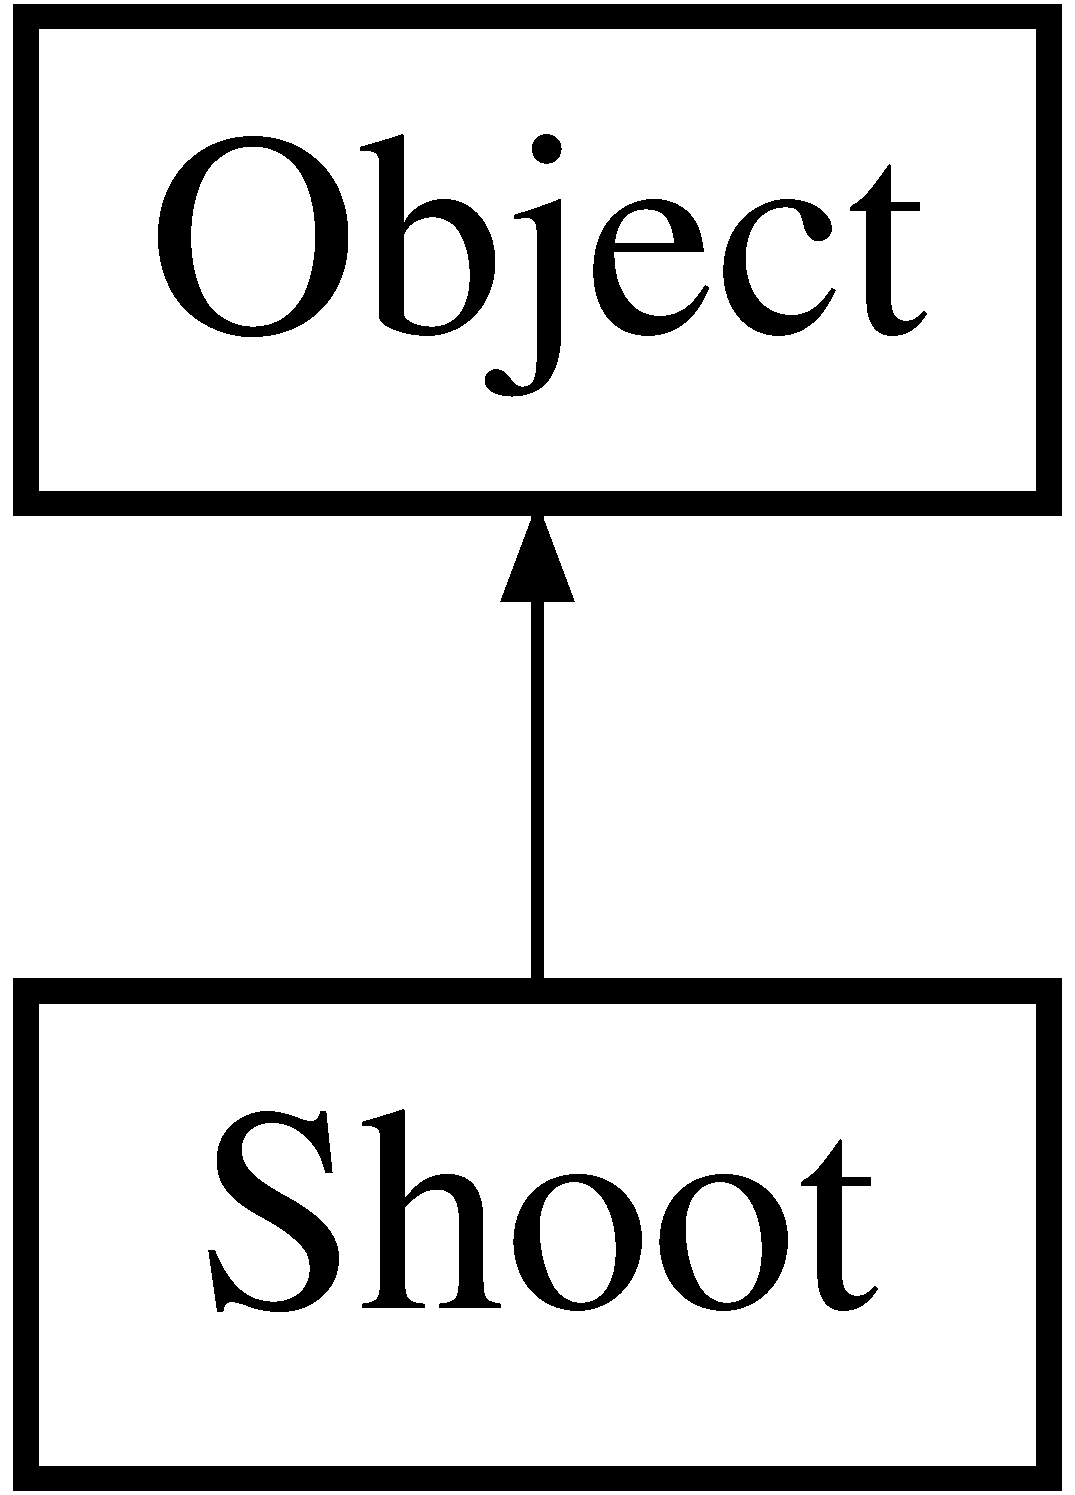
\includegraphics[height=2.000000cm]{class_shoot}
\end{center}
\end{figure}
\subsection*{Fonctions membres publiques}
\begin{DoxyCompactItemize}
\item 
\hyperlink{class_shoot_a13490e5d90536aecbceb753e11879a5b}{Shoot} ()
\end{DoxyCompactItemize}


\subsection{Documentation des constructeurs et destructeur}
\mbox{\Hypertarget{class_shoot_a13490e5d90536aecbceb753e11879a5b}\label{class_shoot_a13490e5d90536aecbceb753e11879a5b}} 
\index{Shoot@{Shoot}!Shoot@{Shoot}}
\index{Shoot@{Shoot}!Shoot@{Shoot}}
\subsubsection{\texorpdfstring{Shoot()}{Shoot()}}
{\footnotesize\ttfamily Shoot\+::\+Shoot (\begin{DoxyParamCaption}{ }\end{DoxyParamCaption})}



La documentation de cette classe a été générée à partir des fichiers suivants \+:\begin{DoxyCompactItemize}
\item 
C\+:/\+Users/\+Ragnar\+L/\+Documents/p1408299-\/p1309837/\+Revenges\+Island/src/core/\hyperlink{_shoot_8h}{Shoot.\+h}\item 
C\+:/\+Users/\+Ragnar\+L/\+Documents/p1408299-\/p1309837/\+Revenges\+Island/src/core/\hyperlink{_shoot_8cpp}{Shoot.\+cpp}\end{DoxyCompactItemize}

\hypertarget{class_terrain}{}\section{Référence de la classe Terrain}
\label{class_terrain}\index{Terrain@{Terrain}}


{\ttfamily \#include $<$Terrain.\+h$>$}

\subsection*{Fonctions membres publiques}
\begin{DoxyCompactItemize}
\item 
\hyperlink{class_terrain_a7160a06ab07a86ed97d23374405e8ef6}{Terrain} ()
\item 
\hyperlink{class_terrain_a986a374fb1ab7cbe52b3ba68934bae8c}{Terrain} (int niveau)
\item 
bool \hyperlink{class_terrain_a939a702645ade7ce599f55c1b760cb26}{est\+Position\+Valide} (const int x, const int y) const
\item 
char \hyperlink{class_terrain_a60a33d464cfb8468e26f1b4dee525178}{get\+XY} (const int x, const int y) const
\item 
int \hyperlink{class_terrain_accb6cc4ab37641b10d6d0cc3c2d9b0cb}{get\+DimX} () const
\item 
int \hyperlink{class_terrain_a60bc76d822c15ca30576bd747d156b48}{get\+DimY} () const
\item 
int \hyperlink{class_terrain_a4e44d60542cfb60119468af5d24b69cd}{get\+Num\+Ter} () const
\item 
void \hyperlink{class_terrain_a8982e144bbc068fb1904092edf327d75}{set\+Num\+Ter} (int n)
\item 
void \hyperlink{class_terrain_a52c2a50f1df6a2b67dc411a5ae76ae68}{Change\+Map} (int niveau)
\item 
void \hyperlink{class_terrain_a97e790dd5379c05db3515d90b2f54b02}{set\+DimX} (int x)
\item 
void \hyperlink{class_terrain_a4fad5f05f2d96ca8ad0cb6442c218df4}{set\+DimY} (int y)
\end{DoxyCompactItemize}
\subsection*{Attributs privés}
\begin{DoxyCompactItemize}
\item 
int \hyperlink{class_terrain_a3daf4955d95ede05eca8addab03445cd}{dimx}
\item 
int \hyperlink{class_terrain_a8ffa11e67f45e16389333431fab2110f}{dimy}
\item 
char \hyperlink{class_terrain_a52f0fcf1c339c1c5ac1fb9b3146b8d75}{ter} \mbox{[}100\mbox{]}\mbox{[}100\mbox{]}
\end{DoxyCompactItemize}


\subsection{Documentation des constructeurs et destructeur}
\mbox{\Hypertarget{class_terrain_a7160a06ab07a86ed97d23374405e8ef6}\label{class_terrain_a7160a06ab07a86ed97d23374405e8ef6}} 
\index{Terrain@{Terrain}!Terrain@{Terrain}}
\index{Terrain@{Terrain}!Terrain@{Terrain}}
\subsubsection{\texorpdfstring{Terrain()}{Terrain()}\hspace{0.1cm}{\footnotesize\ttfamily [1/2]}}
{\footnotesize\ttfamily Terrain\+::\+Terrain (\begin{DoxyParamCaption}{ }\end{DoxyParamCaption})}

\mbox{\Hypertarget{class_terrain_a986a374fb1ab7cbe52b3ba68934bae8c}\label{class_terrain_a986a374fb1ab7cbe52b3ba68934bae8c}} 
\index{Terrain@{Terrain}!Terrain@{Terrain}}
\index{Terrain@{Terrain}!Terrain@{Terrain}}
\subsubsection{\texorpdfstring{Terrain()}{Terrain()}\hspace{0.1cm}{\footnotesize\ttfamily [2/2]}}
{\footnotesize\ttfamily Terrain\+::\+Terrain (\begin{DoxyParamCaption}\item[{int}]{niveau }\end{DoxyParamCaption})}



\subsection{Documentation des fonctions membres}
\mbox{\Hypertarget{class_terrain_a52c2a50f1df6a2b67dc411a5ae76ae68}\label{class_terrain_a52c2a50f1df6a2b67dc411a5ae76ae68}} 
\index{Terrain@{Terrain}!Change\+Map@{Change\+Map}}
\index{Change\+Map@{Change\+Map}!Terrain@{Terrain}}
\subsubsection{\texorpdfstring{Change\+Map()}{ChangeMap()}}
{\footnotesize\ttfamily void Terrain\+::\+Change\+Map (\begin{DoxyParamCaption}\item[{int}]{niveau }\end{DoxyParamCaption})}

\mbox{\Hypertarget{class_terrain_a939a702645ade7ce599f55c1b760cb26}\label{class_terrain_a939a702645ade7ce599f55c1b760cb26}} 
\index{Terrain@{Terrain}!est\+Position\+Valide@{est\+Position\+Valide}}
\index{est\+Position\+Valide@{est\+Position\+Valide}!Terrain@{Terrain}}
\subsubsection{\texorpdfstring{est\+Position\+Valide()}{estPositionValide()}}
{\footnotesize\ttfamily bool Terrain\+::est\+Position\+Valide (\begin{DoxyParamCaption}\item[{const int}]{x,  }\item[{const int}]{y }\end{DoxyParamCaption}) const}

\mbox{\Hypertarget{class_terrain_accb6cc4ab37641b10d6d0cc3c2d9b0cb}\label{class_terrain_accb6cc4ab37641b10d6d0cc3c2d9b0cb}} 
\index{Terrain@{Terrain}!get\+DimX@{get\+DimX}}
\index{get\+DimX@{get\+DimX}!Terrain@{Terrain}}
\subsubsection{\texorpdfstring{get\+Dim\+X()}{getDimX()}}
{\footnotesize\ttfamily int Terrain\+::get\+DimX (\begin{DoxyParamCaption}{ }\end{DoxyParamCaption}) const}

\mbox{\Hypertarget{class_terrain_a60bc76d822c15ca30576bd747d156b48}\label{class_terrain_a60bc76d822c15ca30576bd747d156b48}} 
\index{Terrain@{Terrain}!get\+DimY@{get\+DimY}}
\index{get\+DimY@{get\+DimY}!Terrain@{Terrain}}
\subsubsection{\texorpdfstring{get\+Dim\+Y()}{getDimY()}}
{\footnotesize\ttfamily int Terrain\+::get\+DimY (\begin{DoxyParamCaption}{ }\end{DoxyParamCaption}) const}

\mbox{\Hypertarget{class_terrain_a4e44d60542cfb60119468af5d24b69cd}\label{class_terrain_a4e44d60542cfb60119468af5d24b69cd}} 
\index{Terrain@{Terrain}!get\+Num\+Ter@{get\+Num\+Ter}}
\index{get\+Num\+Ter@{get\+Num\+Ter}!Terrain@{Terrain}}
\subsubsection{\texorpdfstring{get\+Num\+Ter()}{getNumTer()}}
{\footnotesize\ttfamily int Terrain\+::get\+Num\+Ter (\begin{DoxyParamCaption}{ }\end{DoxyParamCaption}) const}

\mbox{\Hypertarget{class_terrain_a60a33d464cfb8468e26f1b4dee525178}\label{class_terrain_a60a33d464cfb8468e26f1b4dee525178}} 
\index{Terrain@{Terrain}!get\+XY@{get\+XY}}
\index{get\+XY@{get\+XY}!Terrain@{Terrain}}
\subsubsection{\texorpdfstring{get\+X\+Y()}{getXY()}}
{\footnotesize\ttfamily char Terrain\+::get\+XY (\begin{DoxyParamCaption}\item[{const int}]{x,  }\item[{const int}]{y }\end{DoxyParamCaption}) const}

\mbox{\Hypertarget{class_terrain_a97e790dd5379c05db3515d90b2f54b02}\label{class_terrain_a97e790dd5379c05db3515d90b2f54b02}} 
\index{Terrain@{Terrain}!set\+DimX@{set\+DimX}}
\index{set\+DimX@{set\+DimX}!Terrain@{Terrain}}
\subsubsection{\texorpdfstring{set\+Dim\+X()}{setDimX()}}
{\footnotesize\ttfamily void Terrain\+::set\+DimX (\begin{DoxyParamCaption}\item[{int}]{x }\end{DoxyParamCaption})}

\mbox{\Hypertarget{class_terrain_a4fad5f05f2d96ca8ad0cb6442c218df4}\label{class_terrain_a4fad5f05f2d96ca8ad0cb6442c218df4}} 
\index{Terrain@{Terrain}!set\+DimY@{set\+DimY}}
\index{set\+DimY@{set\+DimY}!Terrain@{Terrain}}
\subsubsection{\texorpdfstring{set\+Dim\+Y()}{setDimY()}}
{\footnotesize\ttfamily void Terrain\+::set\+DimY (\begin{DoxyParamCaption}\item[{int}]{y }\end{DoxyParamCaption})}

\mbox{\Hypertarget{class_terrain_a8982e144bbc068fb1904092edf327d75}\label{class_terrain_a8982e144bbc068fb1904092edf327d75}} 
\index{Terrain@{Terrain}!set\+Num\+Ter@{set\+Num\+Ter}}
\index{set\+Num\+Ter@{set\+Num\+Ter}!Terrain@{Terrain}}
\subsubsection{\texorpdfstring{set\+Num\+Ter()}{setNumTer()}}
{\footnotesize\ttfamily void Terrain\+::set\+Num\+Ter (\begin{DoxyParamCaption}\item[{int}]{n }\end{DoxyParamCaption})}



\subsection{Documentation des données membres}
\mbox{\Hypertarget{class_terrain_a3daf4955d95ede05eca8addab03445cd}\label{class_terrain_a3daf4955d95ede05eca8addab03445cd}} 
\index{Terrain@{Terrain}!dimx@{dimx}}
\index{dimx@{dimx}!Terrain@{Terrain}}
\subsubsection{\texorpdfstring{dimx}{dimx}}
{\footnotesize\ttfamily int Terrain\+::dimx\hspace{0.3cm}{\ttfamily [private]}}

\mbox{\Hypertarget{class_terrain_a8ffa11e67f45e16389333431fab2110f}\label{class_terrain_a8ffa11e67f45e16389333431fab2110f}} 
\index{Terrain@{Terrain}!dimy@{dimy}}
\index{dimy@{dimy}!Terrain@{Terrain}}
\subsubsection{\texorpdfstring{dimy}{dimy}}
{\footnotesize\ttfamily int Terrain\+::dimy\hspace{0.3cm}{\ttfamily [private]}}

\mbox{\Hypertarget{class_terrain_a52f0fcf1c339c1c5ac1fb9b3146b8d75}\label{class_terrain_a52f0fcf1c339c1c5ac1fb9b3146b8d75}} 
\index{Terrain@{Terrain}!ter@{ter}}
\index{ter@{ter}!Terrain@{Terrain}}
\subsubsection{\texorpdfstring{ter}{ter}}
{\footnotesize\ttfamily char Terrain\+::ter\mbox{[}100\mbox{]}\mbox{[}100\mbox{]}\hspace{0.3cm}{\ttfamily [private]}}



La documentation de cette classe a été générée à partir des fichiers suivants \+:\begin{DoxyCompactItemize}
\item 
C\+:/\+Users/\+Ragnar\+L/\+Documents/p1408299-\/p1309837/\+Revenges\+Island/src/core/\hyperlink{_terrain_8h}{Terrain.\+h}\item 
C\+:/\+Users/\+Ragnar\+L/\+Documents/p1408299-\/p1309837/\+Revenges\+Island/src/core/\hyperlink{_terrain_8cpp}{Terrain.\+cpp}\end{DoxyCompactItemize}

\hypertarget{class_win_t_x_t}{}\section{Référence de la classe Win\+T\+XT}
\label{class_win_t_x_t}\index{Win\+T\+XT@{Win\+T\+XT}}


une fen�tre texte est un tableau 2D de caract�res  




{\ttfamily \#include $<$win\+Txt.\+h$>$}

\subsection*{Fonctions membres publiques}
\begin{DoxyCompactItemize}
\item 
\hyperlink{class_win_t_x_t_a20dfee2e4ee2bef4379e86289f416b1c}{Win\+T\+XT} ()
\item 
\hyperlink{class_win_t_x_t_ad471ddd48d2a7c43acccd1204e419527}{Win\+T\+XT} (int dx, int dy)
\item 
void \hyperlink{class_win_t_x_t_a1b4cb203533f78bed29498591631f436}{clear} (char c=\textquotesingle{} \textquotesingle{})
\item 
void \hyperlink{class_win_t_x_t_a407cce45e7f81546540f4f8a9b85ce45}{print} (int x, int y, char c)
\item 
void \hyperlink{class_win_t_x_t_ad021d5fb9862b9ea7985f8cef50451e2}{print} (int x, int y, char $\ast$c)
\item 
void \hyperlink{class_win_t_x_t_af83a18827593465fc397983c97b4e886}{draw} (int x=0, int y=0)
\item 
void \hyperlink{class_win_t_x_t_a3e8793fd263bb51a62ec8a5e89904c49}{pause} ()
\item 
char \hyperlink{class_win_t_x_t_a418c66475403586ac57a80eceb409166}{get\+Ch} ()
\end{DoxyCompactItemize}
\subsection*{Attributs privés}
\begin{DoxyCompactItemize}
\item 
int \hyperlink{class_win_t_x_t_aae9dd786d11da5b46de6f4ea3041a0ab}{dimx}
\begin{DoxyCompactList}\small\item\em largeur \end{DoxyCompactList}\item 
int \hyperlink{class_win_t_x_t_ab94c58aaf938cf5e119553ee918b9a19}{dimy}
\begin{DoxyCompactList}\small\item\em heuteur \end{DoxyCompactList}\item 
char $\ast$ \hyperlink{class_win_t_x_t_ace5ef6c746d586385fcea85073bd1d41}{win}
\begin{DoxyCompactList}\small\item\em stocke le contenu de la fen�tre dans un tableau 1D mais on y accede en 2D \end{DoxyCompactList}\end{DoxyCompactItemize}


\subsection{Description détaillée}
une fen�tre texte est un tableau 2D de caract�res 

\subsection{Documentation des constructeurs et destructeur}
\mbox{\Hypertarget{class_win_t_x_t_a20dfee2e4ee2bef4379e86289f416b1c}\label{class_win_t_x_t_a20dfee2e4ee2bef4379e86289f416b1c}} 
\index{Win\+T\+XT@{Win\+T\+XT}!Win\+T\+XT@{Win\+T\+XT}}
\index{Win\+T\+XT@{Win\+T\+XT}!Win\+T\+XT@{Win\+T\+XT}}
\subsubsection{\texorpdfstring{Win\+T\+X\+T()}{WinTXT()}\hspace{0.1cm}{\footnotesize\ttfamily [1/2]}}
{\footnotesize\ttfamily Win\+T\+X\+T\+::\+Win\+T\+XT (\begin{DoxyParamCaption}{ }\end{DoxyParamCaption})}

\mbox{\Hypertarget{class_win_t_x_t_ad471ddd48d2a7c43acccd1204e419527}\label{class_win_t_x_t_ad471ddd48d2a7c43acccd1204e419527}} 
\index{Win\+T\+XT@{Win\+T\+XT}!Win\+T\+XT@{Win\+T\+XT}}
\index{Win\+T\+XT@{Win\+T\+XT}!Win\+T\+XT@{Win\+T\+XT}}
\subsubsection{\texorpdfstring{Win\+T\+X\+T()}{WinTXT()}\hspace{0.1cm}{\footnotesize\ttfamily [2/2]}}
{\footnotesize\ttfamily Win\+T\+X\+T\+::\+Win\+T\+XT (\begin{DoxyParamCaption}\item[{int}]{dx,  }\item[{int}]{dy }\end{DoxyParamCaption})}



\subsection{Documentation des fonctions membres}
\mbox{\Hypertarget{class_win_t_x_t_a1b4cb203533f78bed29498591631f436}\label{class_win_t_x_t_a1b4cb203533f78bed29498591631f436}} 
\index{Win\+T\+XT@{Win\+T\+XT}!clear@{clear}}
\index{clear@{clear}!Win\+T\+XT@{Win\+T\+XT}}
\subsubsection{\texorpdfstring{clear()}{clear()}}
{\footnotesize\ttfamily void Win\+T\+X\+T\+::clear (\begin{DoxyParamCaption}\item[{char}]{c = {\ttfamily \textquotesingle{}~\textquotesingle{}} }\end{DoxyParamCaption})}

\mbox{\Hypertarget{class_win_t_x_t_af83a18827593465fc397983c97b4e886}\label{class_win_t_x_t_af83a18827593465fc397983c97b4e886}} 
\index{Win\+T\+XT@{Win\+T\+XT}!draw@{draw}}
\index{draw@{draw}!Win\+T\+XT@{Win\+T\+XT}}
\subsubsection{\texorpdfstring{draw()}{draw()}}
{\footnotesize\ttfamily void Win\+T\+X\+T\+::draw (\begin{DoxyParamCaption}\item[{int}]{x = {\ttfamily 0},  }\item[{int}]{y = {\ttfamily 0} }\end{DoxyParamCaption})}

\mbox{\Hypertarget{class_win_t_x_t_a418c66475403586ac57a80eceb409166}\label{class_win_t_x_t_a418c66475403586ac57a80eceb409166}} 
\index{Win\+T\+XT@{Win\+T\+XT}!get\+Ch@{get\+Ch}}
\index{get\+Ch@{get\+Ch}!Win\+T\+XT@{Win\+T\+XT}}
\subsubsection{\texorpdfstring{get\+Ch()}{getCh()}}
{\footnotesize\ttfamily char Win\+T\+X\+T\+::get\+Ch (\begin{DoxyParamCaption}{ }\end{DoxyParamCaption})}

\mbox{\Hypertarget{class_win_t_x_t_a3e8793fd263bb51a62ec8a5e89904c49}\label{class_win_t_x_t_a3e8793fd263bb51a62ec8a5e89904c49}} 
\index{Win\+T\+XT@{Win\+T\+XT}!pause@{pause}}
\index{pause@{pause}!Win\+T\+XT@{Win\+T\+XT}}
\subsubsection{\texorpdfstring{pause()}{pause()}}
{\footnotesize\ttfamily void Win\+T\+X\+T\+::pause (\begin{DoxyParamCaption}{ }\end{DoxyParamCaption})}

\mbox{\Hypertarget{class_win_t_x_t_a407cce45e7f81546540f4f8a9b85ce45}\label{class_win_t_x_t_a407cce45e7f81546540f4f8a9b85ce45}} 
\index{Win\+T\+XT@{Win\+T\+XT}!print@{print}}
\index{print@{print}!Win\+T\+XT@{Win\+T\+XT}}
\subsubsection{\texorpdfstring{print()}{print()}\hspace{0.1cm}{\footnotesize\ttfamily [1/2]}}
{\footnotesize\ttfamily void Win\+T\+X\+T\+::print (\begin{DoxyParamCaption}\item[{int}]{x,  }\item[{int}]{y,  }\item[{char}]{c }\end{DoxyParamCaption})}

\mbox{\Hypertarget{class_win_t_x_t_ad021d5fb9862b9ea7985f8cef50451e2}\label{class_win_t_x_t_ad021d5fb9862b9ea7985f8cef50451e2}} 
\index{Win\+T\+XT@{Win\+T\+XT}!print@{print}}
\index{print@{print}!Win\+T\+XT@{Win\+T\+XT}}
\subsubsection{\texorpdfstring{print()}{print()}\hspace{0.1cm}{\footnotesize\ttfamily [2/2]}}
{\footnotesize\ttfamily void Win\+T\+X\+T\+::print (\begin{DoxyParamCaption}\item[{int}]{x,  }\item[{int}]{y,  }\item[{char $\ast$}]{c }\end{DoxyParamCaption})}



\subsection{Documentation des données membres}
\mbox{\Hypertarget{class_win_t_x_t_aae9dd786d11da5b46de6f4ea3041a0ab}\label{class_win_t_x_t_aae9dd786d11da5b46de6f4ea3041a0ab}} 
\index{Win\+T\+XT@{Win\+T\+XT}!dimx@{dimx}}
\index{dimx@{dimx}!Win\+T\+XT@{Win\+T\+XT}}
\subsubsection{\texorpdfstring{dimx}{dimx}}
{\footnotesize\ttfamily int Win\+T\+X\+T\+::dimx\hspace{0.3cm}{\ttfamily [private]}}



largeur 

\mbox{\Hypertarget{class_win_t_x_t_ab94c58aaf938cf5e119553ee918b9a19}\label{class_win_t_x_t_ab94c58aaf938cf5e119553ee918b9a19}} 
\index{Win\+T\+XT@{Win\+T\+XT}!dimy@{dimy}}
\index{dimy@{dimy}!Win\+T\+XT@{Win\+T\+XT}}
\subsubsection{\texorpdfstring{dimy}{dimy}}
{\footnotesize\ttfamily int Win\+T\+X\+T\+::dimy\hspace{0.3cm}{\ttfamily [private]}}



heuteur 

\mbox{\Hypertarget{class_win_t_x_t_ace5ef6c746d586385fcea85073bd1d41}\label{class_win_t_x_t_ace5ef6c746d586385fcea85073bd1d41}} 
\index{Win\+T\+XT@{Win\+T\+XT}!win@{win}}
\index{win@{win}!Win\+T\+XT@{Win\+T\+XT}}
\subsubsection{\texorpdfstring{win}{win}}
{\footnotesize\ttfamily char$\ast$ Win\+T\+X\+T\+::win\hspace{0.3cm}{\ttfamily [private]}}



stocke le contenu de la fen�tre dans un tableau 1D mais on y accede en 2D 



La documentation de cette classe a été générée à partir des fichiers suivants \+:\begin{DoxyCompactItemize}
\item 
C\+:/\+Users/\+Ragnar\+L/\+Documents/p1408299-\/p1309837/\+Revenges\+Island/src/txt/\hyperlink{win_txt_8h}{win\+Txt.\+h}\item 
C\+:/\+Users/\+Ragnar\+L/\+Documents/p1408299-\/p1309837/\+Revenges\+Island/src/txt/\hyperlink{win_txt_8cpp}{win\+Txt.\+cpp}\end{DoxyCompactItemize}

\chapter{Documentation des fichiers}
\hypertarget{_ennemi_8cpp}{}\section{Référence du fichier C\+:/\+Users/\+Ragnar\+L/\+Documents/p1408299-\/p1309837/\+Revenges\+Island/src/core/\+Ennemi.cpp}
\label{_ennemi_8cpp}\index{C\+:/\+Users/\+Ragnar\+L/\+Documents/p1408299-\/p1309837/\+Revenges\+Island/src/core/\+Ennemi.\+cpp@{C\+:/\+Users/\+Ragnar\+L/\+Documents/p1408299-\/p1309837/\+Revenges\+Island/src/core/\+Ennemi.\+cpp}}
{\ttfamily \#include \char`\"{}Ennemi.\+h\char`\"{}}\newline
{\ttfamily \#include $<$stdlib.\+h$>$}\newline
{\ttfamily \#include $<$assert.\+h$>$}\newline
{\ttfamily \#include $<$iostream$>$}\newline
{\ttfamily \#include \char`\"{}Shoot.\+h\char`\"{}}\newline

\hypertarget{_ennemi_8h}{}\section{Référence du fichier C\+:/\+Users/\+Ragnar\+L/\+Documents/p1408299-\/p1309837/\+Revenges\+Island/src/core/\+Ennemi.h}
\label{_ennemi_8h}\index{C\+:/\+Users/\+Ragnar\+L/\+Documents/p1408299-\/p1309837/\+Revenges\+Island/src/core/\+Ennemi.\+h@{C\+:/\+Users/\+Ragnar\+L/\+Documents/p1408299-\/p1309837/\+Revenges\+Island/src/core/\+Ennemi.\+h}}


Fichier d\textquotesingle{}entete du module \hyperlink{class_ennemi}{Ennemi}.  


{\ttfamily \#include $<$iostream$>$}\newline
{\ttfamily \#include \char`\"{}Terrain.\+h\char`\"{}}\newline
{\ttfamily \#include \char`\"{}Shoot.\+h\char`\"{}}\newline
{\ttfamily \#include \char`\"{}Navigateur.\+h\char`\"{}}\newline
{\ttfamily \#include \char`\"{}Object.\+h\char`\"{}}\newline
\subsection*{Classes}
\begin{DoxyCompactItemize}
\item 
class \hyperlink{class_ennemi}{Ennemi}
\begin{DoxyCompactList}\small\item\em classe utilisée pour la gestion de l\textquotesingle{}\hyperlink{class_ennemi}{Ennemi}. \hyperlink{class_ennemi}{Ennemi} hérite de la classe \hyperlink{class_object}{Object}. \end{DoxyCompactList}\end{DoxyCompactItemize}


\subsection{Description détaillée}
Fichier d\textquotesingle{}entete du module \hyperlink{class_ennemi}{Ennemi}. 

Prototype du module \hyperlink{class_ennemi}{Ennemi}.

\begin{DoxyAuthor}{Auteur}
D\+J\+E\+B\+A\+R\+N\+I-\/\+B\+E\+L\+T\+R\+AN 
\end{DoxyAuthor}
\begin{DoxyVersion}{Version}
1.\+0 
\end{DoxyVersion}

\hypertarget{_equipage_8cpp}{}\section{Référence du fichier C\+:/\+Users/\+Ragnar\+L/\+Documents/p1408299-\/p1309837/\+Revenges\+Island/src/core/\+Equipage.cpp}
\label{_equipage_8cpp}\index{C\+:/\+Users/\+Ragnar\+L/\+Documents/p1408299-\/p1309837/\+Revenges\+Island/src/core/\+Equipage.\+cpp@{C\+:/\+Users/\+Ragnar\+L/\+Documents/p1408299-\/p1309837/\+Revenges\+Island/src/core/\+Equipage.\+cpp}}
{\ttfamily \#include \char`\"{}Equipage.\+h\char`\"{}}\newline
{\ttfamily \#include $<$stdlib.\+h$>$}\newline
{\ttfamily \#include $<$assert.\+h$>$}\newline
{\ttfamily \#include $<$iostream$>$}\newline

\hypertarget{_equipage_8h}{}\section{Référence du fichier C\+:/\+Users/\+Ragnar\+L/\+Documents/p1408299-\/p1309837/\+Revenges\+Island/src/core/\+Equipage.h}
\label{_equipage_8h}\index{C\+:/\+Users/\+Ragnar\+L/\+Documents/p1408299-\/p1309837/\+Revenges\+Island/src/core/\+Equipage.\+h@{C\+:/\+Users/\+Ragnar\+L/\+Documents/p1408299-\/p1309837/\+Revenges\+Island/src/core/\+Equipage.\+h}}


Fichier d\textquotesingle{}entete du module \hyperlink{class_equipage}{Equipage}.  


{\ttfamily \#include \char`\"{}Terrain.\+h\char`\"{}}\newline
{\ttfamily \#include \char`\"{}Object.\+h\char`\"{}}\newline
{\ttfamily \#include \char`\"{}Ennemi.\+h\char`\"{}}\newline
\subsection*{Classes}
\begin{DoxyCompactItemize}
\item 
class \hyperlink{class_equipage}{Equipage}
\begin{DoxyCompactList}\small\item\em classe utilisée pour la gestion de l\textquotesingle{}\hyperlink{class_equipage}{Equipage}. \hyperlink{class_equipage}{Equipage} hérite de la classe \hyperlink{class_object}{Object}. \end{DoxyCompactList}\end{DoxyCompactItemize}


\subsection{Description détaillée}
Fichier d\textquotesingle{}entete du module \hyperlink{class_equipage}{Equipage}. 

Prototype du module \hyperlink{class_equipage}{Equipage}.

\begin{DoxyAuthor}{Auteur}
D\+J\+E\+B\+A\+R\+N\+I-\/\+B\+E\+L\+T\+R\+AN 
\end{DoxyAuthor}
\begin{DoxyVersion}{Version}
1.\+0 
\end{DoxyVersion}

\hypertarget{_jeu_8cpp}{}\section{Référence du fichier C\+:/\+Users/\+Ragnar\+L/\+Documents/p1408299-\/p1309837/\+Revenges\+Island/src/core/\+Jeu.cpp}
\label{_jeu_8cpp}\index{C\+:/\+Users/\+Ragnar\+L/\+Documents/p1408299-\/p1309837/\+Revenges\+Island/src/core/\+Jeu.\+cpp@{C\+:/\+Users/\+Ragnar\+L/\+Documents/p1408299-\/p1309837/\+Revenges\+Island/src/core/\+Jeu.\+cpp}}
{\ttfamily \#include \char`\"{}Jeu.\+h\char`\"{}}\newline
{\ttfamily \#include $<$iostream$>$}\newline
{\ttfamily \#include $<$string$>$}\newline
{\ttfamily \#include $<$assert.\+h$>$}\newline
\subsection*{Macros}
\begin{DoxyCompactItemize}
\item 
\#define \hyperlink{_jeu_8cpp_ac66768ecf619e4b9428d1e64b13b3d32}{F\+I\+R\+E\+B\+A\+L\+L\+S\+\_\+\+M\+AX}~3
\end{DoxyCompactItemize}


\subsection{Documentation des macros}
\mbox{\Hypertarget{_jeu_8cpp_ac66768ecf619e4b9428d1e64b13b3d32}\label{_jeu_8cpp_ac66768ecf619e4b9428d1e64b13b3d32}} 
\index{Jeu.\+cpp@{Jeu.\+cpp}!F\+I\+R\+E\+B\+A\+L\+L\+S\+\_\+\+M\+AX@{F\+I\+R\+E\+B\+A\+L\+L\+S\+\_\+\+M\+AX}}
\index{F\+I\+R\+E\+B\+A\+L\+L\+S\+\_\+\+M\+AX@{F\+I\+R\+E\+B\+A\+L\+L\+S\+\_\+\+M\+AX}!Jeu.\+cpp@{Jeu.\+cpp}}
\subsubsection{\texorpdfstring{F\+I\+R\+E\+B\+A\+L\+L\+S\+\_\+\+M\+AX}{FIREBALLS\_MAX}}
{\footnotesize\ttfamily \#define F\+I\+R\+E\+B\+A\+L\+L\+S\+\_\+\+M\+AX~3}


\hypertarget{_jeu_8h}{}\section{Référence du fichier C\+:/\+Users/\+Ragnar\+L/\+Documents/p1408299-\/p1309837/\+Revenges\+Island/src/core/\+Jeu.h}
\label{_jeu_8h}\index{C\+:/\+Users/\+Ragnar\+L/\+Documents/p1408299-\/p1309837/\+Revenges\+Island/src/core/\+Jeu.\+h@{C\+:/\+Users/\+Ragnar\+L/\+Documents/p1408299-\/p1309837/\+Revenges\+Island/src/core/\+Jeu.\+h}}


Fichier d\textquotesingle{}entete du module \hyperlink{class_jeu}{Jeu}.  


{\ttfamily \#include \char`\"{}Navigateur.\+h\char`\"{}}\newline
{\ttfamily \#include \char`\"{}Terrain.\+h\char`\"{}}\newline
{\ttfamily \#include \char`\"{}Ennemi.\+h\char`\"{}}\newline
{\ttfamily \#include \char`\"{}Equipage.\+h\char`\"{}}\newline
{\ttfamily \#include \char`\"{}Shoot.\+h\char`\"{}}\newline
{\ttfamily \#include \char`\"{}../txt/win\+Txt.\+h\char`\"{}}\newline
\subsection*{Classes}
\begin{DoxyCompactItemize}
\item 
class \hyperlink{class_jeu}{Jeu}
\end{DoxyCompactItemize}


\subsection{Description détaillée}
Fichier d\textquotesingle{}entete du module \hyperlink{class_jeu}{Jeu}. 

Prototype du module \hyperlink{class_jeu}{Jeu}.

\begin{DoxyAuthor}{Auteur}
D\+J\+E\+B\+A\+R\+N\+I-\/\+B\+E\+L\+T\+R\+AN 
\end{DoxyAuthor}
\begin{DoxyVersion}{Version}
1.\+0 
\end{DoxyVersion}

\hypertarget{_menu_8cpp}{}\section{Référence du fichier C\+:/\+Users/\+Ragnar\+L/\+Documents/p1408299-\/p1309837/\+Revenges\+Island/src/core/\+Menu.cpp}
\label{_menu_8cpp}\index{C\+:/\+Users/\+Ragnar\+L/\+Documents/p1408299-\/p1309837/\+Revenges\+Island/src/core/\+Menu.\+cpp@{C\+:/\+Users/\+Ragnar\+L/\+Documents/p1408299-\/p1309837/\+Revenges\+Island/src/core/\+Menu.\+cpp}}
{\ttfamily \#include \char`\"{}Menu.\+h\char`\"{}}\newline
{\ttfamily \#include $<$iostream$>$}\newline
{\ttfamily \#include $<$stdio.\+h$>$}\newline

\hypertarget{_menu_8h}{}\section{Référence du fichier C\+:/\+Users/\+Ragnar\+L/\+Documents/p1408299-\/p1309837/\+Revenges\+Island/src/core/\+Menu.h}
\label{_menu_8h}\index{C\+:/\+Users/\+Ragnar\+L/\+Documents/p1408299-\/p1309837/\+Revenges\+Island/src/core/\+Menu.\+h@{C\+:/\+Users/\+Ragnar\+L/\+Documents/p1408299-\/p1309837/\+Revenges\+Island/src/core/\+Menu.\+h}}


Fichier d\textquotesingle{}entete du module \hyperlink{class_menu}{Menu}.  


\subsection*{Classes}
\begin{DoxyCompactItemize}
\item 
class \hyperlink{class_menu}{Menu}
\begin{DoxyCompactList}\small\item\em classe utilisée pour la gestion du \hyperlink{class_menu}{Menu}. \end{DoxyCompactList}\end{DoxyCompactItemize}


\subsection{Description détaillée}
Fichier d\textquotesingle{}entete du module \hyperlink{class_menu}{Menu}. 

Prototype du module \hyperlink{class_menu}{Menu}.

\begin{DoxyAuthor}{Auteur}
D\+J\+E\+B\+A\+R\+N\+I-\/\+B\+E\+L\+T\+R\+AN 
\end{DoxyAuthor}
\begin{DoxyVersion}{Version}
1.\+0 
\end{DoxyVersion}

\hypertarget{_navigateur_8cpp}{}\section{Référence du fichier C\+:/\+Users/\+Ragnar\+L/\+Documents/p1408299-\/p1309837/\+Revenges\+Island/src/core/\+Navigateur.cpp}
\label{_navigateur_8cpp}\index{C\+:/\+Users/\+Ragnar\+L/\+Documents/p1408299-\/p1309837/\+Revenges\+Island/src/core/\+Navigateur.\+cpp@{C\+:/\+Users/\+Ragnar\+L/\+Documents/p1408299-\/p1309837/\+Revenges\+Island/src/core/\+Navigateur.\+cpp}}
{\ttfamily \#include \char`\"{}Navigateur.\+h\char`\"{}}\newline
{\ttfamily \#include $<$assert.\+h$>$}\newline
{\ttfamily \#include $<$iostream$>$}\newline
{\ttfamily \#include $<$stdio.\+h$>$}\newline

\hypertarget{_navigateur_8h}{}\section{Référence du fichier C\+:/\+Users/\+Ragnar\+L/\+Documents/p1408299-\/p1309837/\+Revenges\+Island/src/core/\+Navigateur.h}
\label{_navigateur_8h}\index{C\+:/\+Users/\+Ragnar\+L/\+Documents/p1408299-\/p1309837/\+Revenges\+Island/src/core/\+Navigateur.\+h@{C\+:/\+Users/\+Ragnar\+L/\+Documents/p1408299-\/p1309837/\+Revenges\+Island/src/core/\+Navigateur.\+h}}


Fichier d\textquotesingle{}entete du module \hyperlink{class_navigateur}{Navigateur}.  


{\ttfamily \#include \char`\"{}Terrain.\+h\char`\"{}}\newline
{\ttfamily \#include \char`\"{}Ennemi.\+h\char`\"{}}\newline
{\ttfamily \#include \char`\"{}Object.\+h\char`\"{}}\newline
\subsection*{Classes}
\begin{DoxyCompactItemize}
\item 
class \hyperlink{class_navigateur}{Navigateur}
\begin{DoxyCompactList}\small\item\em classe utilisée pour la gestion du \hyperlink{class_navigateur}{Navigateur(joueur)}. \hyperlink{class_navigateur}{Navigateur} hérite de la classe \hyperlink{class_object}{Object}. \end{DoxyCompactList}\end{DoxyCompactItemize}


\subsection{Description détaillée}
Fichier d\textquotesingle{}entete du module \hyperlink{class_navigateur}{Navigateur}. 

Prototype du module \hyperlink{class_navigateur}{Navigateur}.

\begin{DoxyAuthor}{Auteur}
D\+J\+E\+B\+A\+R\+N\+I-\/\+B\+E\+L\+T\+R\+AN 
\end{DoxyAuthor}
\begin{DoxyVersion}{Version}
1.\+0 
\end{DoxyVersion}

\hypertarget{_object_8cpp}{}\section{Référence du fichier C\+:/\+Users/\+Ragnar\+L/\+Documents/p1408299-\/p1309837/\+Revenges\+Island/src/core/\+Object.cpp}
\label{_object_8cpp}\index{C\+:/\+Users/\+Ragnar\+L/\+Documents/p1408299-\/p1309837/\+Revenges\+Island/src/core/\+Object.\+cpp@{C\+:/\+Users/\+Ragnar\+L/\+Documents/p1408299-\/p1309837/\+Revenges\+Island/src/core/\+Object.\+cpp}}
{\ttfamily \#include \char`\"{}Object.\+h\char`\"{}}\newline

\hypertarget{_object_8h}{}\section{Référence du fichier C\+:/\+Users/\+Ragnar\+L/\+Documents/p1408299-\/p1309837/\+Revenges\+Island/src/core/\+Object.h}
\label{_object_8h}\index{C\+:/\+Users/\+Ragnar\+L/\+Documents/p1408299-\/p1309837/\+Revenges\+Island/src/core/\+Object.\+h@{C\+:/\+Users/\+Ragnar\+L/\+Documents/p1408299-\/p1309837/\+Revenges\+Island/src/core/\+Object.\+h}}


Fichier d\textquotesingle{}entete du module \hyperlink{class_object}{Object}.  


\subsection*{Classes}
\begin{DoxyCompactItemize}
\item 
class \hyperlink{class_object}{Object}
\begin{DoxyCompactList}\small\item\em classe utilisée pour la gestion des Objets. \end{DoxyCompactList}\end{DoxyCompactItemize}


\subsection{Description détaillée}
Fichier d\textquotesingle{}entete du module \hyperlink{class_object}{Object}. 

Prototype du module \hyperlink{class_object}{Object}.

\begin{DoxyAuthor}{Auteur}
D\+J\+E\+B\+A\+R\+N\+I-\/\+B\+E\+L\+T\+R\+AN 
\end{DoxyAuthor}
\begin{DoxyVersion}{Version}
1.\+0 
\end{DoxyVersion}

\hypertarget{_shoot_8cpp}{}\section{Référence du fichier C\+:/\+Users/\+Ragnar\+L/\+Documents/p1408299-\/p1309837/\+Revenges\+Island/src/core/\+Shoot.cpp}
\label{_shoot_8cpp}\index{C\+:/\+Users/\+Ragnar\+L/\+Documents/p1408299-\/p1309837/\+Revenges\+Island/src/core/\+Shoot.\+cpp@{C\+:/\+Users/\+Ragnar\+L/\+Documents/p1408299-\/p1309837/\+Revenges\+Island/src/core/\+Shoot.\+cpp}}
{\ttfamily \#include \char`\"{}Shoot.\+h\char`\"{}}\newline
{\ttfamily \#include $<$assert.\+h$>$}\newline

\hypertarget{_shoot_8h}{}\section{Référence du fichier C\+:/\+Users/\+Ragnar\+L/\+Documents/p1408299-\/p1309837/\+Revenges\+Island/src/core/\+Shoot.h}
\label{_shoot_8h}\index{C\+:/\+Users/\+Ragnar\+L/\+Documents/p1408299-\/p1309837/\+Revenges\+Island/src/core/\+Shoot.\+h@{C\+:/\+Users/\+Ragnar\+L/\+Documents/p1408299-\/p1309837/\+Revenges\+Island/src/core/\+Shoot.\+h}}
{\ttfamily \#include \char`\"{}Terrain.\+h\char`\"{}}\newline
{\ttfamily \#include \char`\"{}Object.\+h\char`\"{}}\newline
\subsection*{Classes}
\begin{DoxyCompactItemize}
\item 
class \hyperlink{class_shoot}{Shoot}
\end{DoxyCompactItemize}

\hypertarget{_terrain_8cpp}{}\section{Référence du fichier C\+:/\+Users/\+Ragnar\+L/\+Documents/p1408299-\/p1309837/\+Revenges\+Island/src/core/\+Terrain.cpp}
\label{_terrain_8cpp}\index{C\+:/\+Users/\+Ragnar\+L/\+Documents/p1408299-\/p1309837/\+Revenges\+Island/src/core/\+Terrain.\+cpp@{C\+:/\+Users/\+Ragnar\+L/\+Documents/p1408299-\/p1309837/\+Revenges\+Island/src/core/\+Terrain.\+cpp}}
{\ttfamily \#include \char`\"{}Terrain.\+h\char`\"{}}\newline
{\ttfamily \#include $<$cassert$>$}\newline
{\ttfamily \#include $<$string$>$}\newline
{\ttfamily \#include $<$iostream$>$}\newline
{\ttfamily \#include $<$stdlib.\+h$>$}\newline
{\ttfamily \#include $<$fstream$>$}\newline
{\ttfamily \#include $<$unistd.\+h$>$}\newline
{\ttfamily \#include $<$stdio.\+h$>$}\newline
\subsection*{Variables}
\begin{DoxyCompactItemize}
\item 
const char \hyperlink{_terrain_8cpp_a7c263001af816247b23f62bbcf71250e}{terrain1} \mbox{[}18\mbox{]}\mbox{[}42\mbox{]}
\item 
const char \hyperlink{_terrain_8cpp_a402e5d8948c47995baf3066d919d3e77}{terrain2} \mbox{[}18\mbox{]}\mbox{[}42\mbox{]}
\item 
const char \hyperlink{_terrain_8cpp_afb373d4eca0d036d9d1315a5c893d922}{terrain3} \mbox{[}18\mbox{]}\mbox{[}42\mbox{]}
\item 
const char \hyperlink{_terrain_8cpp_aea89ec9a2b2b73da6464516926b23bd5}{terrain4} \mbox{[}18\mbox{]}\mbox{[}42\mbox{]}
\end{DoxyCompactItemize}


\subsection{Documentation des variables}
\mbox{\Hypertarget{_terrain_8cpp_a7c263001af816247b23f62bbcf71250e}\label{_terrain_8cpp_a7c263001af816247b23f62bbcf71250e}} 
\index{Terrain.\+cpp@{Terrain.\+cpp}!terrain1@{terrain1}}
\index{terrain1@{terrain1}!Terrain.\+cpp@{Terrain.\+cpp}}
\subsubsection{\texorpdfstring{terrain1}{terrain1}}
{\footnotesize\ttfamily const char terrain1\mbox{[}18\mbox{]}\mbox{[}42\mbox{]}}

{\bfseries Valeur initiale \+:}
\begin{DoxyCode}
=
\{
    \textcolor{stringliteral}{"@@@@@@@@@@@@@@@@@@@@@@@@@@@@@@@@@@@@@@@@"},
    \textcolor{stringliteral}{"@SSSSSSSSSSSSSSSSSSSSSSSSSSSSSSSSV11111@"},
    \textcolor{stringliteral}{"@SSSSSSSSSSSSSSSSSSSSSSSSSSSSSSSSSV1111@"},
    \textcolor{stringliteral}{"@SSSSSSSSSSSSSSSSSSSSSSSSSSSBSSSSSSV111@"},
    \textcolor{stringliteral}{"@SSSSSSSSSSSSSSSSSSSSSSSSSSSBSSSSSV1111@"},
    \textcolor{stringliteral}{"@SSSSSSSSSSSSSSSSSSSSSSSSSSSBSSSSV11111@"},
    \textcolor{stringliteral}{"@SSSSSSSSSSSSSSSSFSSSSSSSSSSSSSSSSV1111@"},
    \textcolor{stringliteral}{"@SSSSSSSSSSSSSSSSSSSSSSSSSSSSSSSSSV1111@"},
    \textcolor{stringliteral}{"@SSSSSSSSSSSSSSSSSSSSBSSSSSSSSSSSV11111@"},
    \textcolor{stringliteral}{"@SSSSSSSSSSSSSSSSFSSSBSSSSSSSSSSSSV1111@"},
    \textcolor{stringliteral}{"@SSSSSSSSSSSSSSSSSSSSBSSSSSSSSSSSSV1111@"},
    \textcolor{stringliteral}{"@SSSSSSSSSSSSSSSSSSSSSSSSSSSSSSSSV11111@"},
    \textcolor{stringliteral}{"@SSSSSSSSSSSSSSSSFSSSSSSSSSSSSSSSSV1111@"},
    \textcolor{stringliteral}{"@SSSSSSSSSSSSSSSSSSSSSSSSSSSBSSSSSV1111@"},
    \textcolor{stringliteral}{"@SSSSSSSSSSSSSSSSSSSSSSSSSSSBSSSSSSV111@"},
    \textcolor{stringliteral}{"@SSSSSSSSSSSSSSSSSSSSSSSSSSSBSSSSSV1111@"},
    \textcolor{stringliteral}{"@SSSSSSSSSSSSSSSSSSSSSSSSSSSSSSSSV11111@"},
    \textcolor{stringliteral}{"@@@@@@@@@@@@@@@@@@@@@@@@@@@@@@@@@@@@@@@@"}
\}
\end{DoxyCode}
\mbox{\Hypertarget{_terrain_8cpp_a402e5d8948c47995baf3066d919d3e77}\label{_terrain_8cpp_a402e5d8948c47995baf3066d919d3e77}} 
\index{Terrain.\+cpp@{Terrain.\+cpp}!terrain2@{terrain2}}
\index{terrain2@{terrain2}!Terrain.\+cpp@{Terrain.\+cpp}}
\subsubsection{\texorpdfstring{terrain2}{terrain2}}
{\footnotesize\ttfamily const char terrain2\mbox{[}18\mbox{]}\mbox{[}42\mbox{]}}

{\bfseries Valeur initiale \+:}
\begin{DoxyCode}
=
\{
    \textcolor{stringliteral}{"@@@@@@@@@@@@@@@@@@@@@@@@@@@@@@@@@@@@@@@@"},
    \textcolor{stringliteral}{"@HAHHHHAHHHHAHHHHAHHHHAHHHHAHHHHAHHHHAH@"},
    \textcolor{stringliteral}{"@HHHHFHHHHFHHHHFHHHHFHHHHFHHHHFHHHHFHHH@"},
    \textcolor{stringliteral}{"@HHHHHHHHHHHHHHHHHHHHHHHHHHHHHHHHHHHHHH@"},
    \textcolor{stringliteral}{"@HHHHAHHHHAHHHHAHHHHAHHHHAHHHHAHHHHAHHH@"},
    \textcolor{stringliteral}{"@HAHHHHAHHHHAHHHHAHHHHAHHHHAHHHHAHHHHAH@"},
    \textcolor{stringliteral}{"@HHHHFHHHHFHHHHFHHHHFHHHHFHHHHFHHHHFHHH@"},
    \textcolor{stringliteral}{"@HFHHHHFHHHHFHHHHFHHHHFHHHHFHHHHFHHHHFH@"},
    \textcolor{stringliteral}{"@HHHHAHHHHAHHHHAHHHHAHHHHAHHHHAHHHHAHHH@"},
    \textcolor{stringliteral}{"@HAHHHHAHHHHAHHHHAHHHHAHHHHAHHHHAHHHHAH@"},
    \textcolor{stringliteral}{"@HHHHFHHHHFHHHHFHHHHFHHHHFHHHHFHHHHFHHH@"},
    \textcolor{stringliteral}{"@HFHHHHFHHHHFHHHHFHHHHFHHHHFHHHHFHHHHFH@"},
    \textcolor{stringliteral}{"@HHHHAHHHHAHHHHAHHHHAHHHHAHHHHAHHHHAHHH@"},
    \textcolor{stringliteral}{"@HAHHHHAHHHHAHHHHAHHHHAHHHHAHHHHAHHHHAH@"},
    \textcolor{stringliteral}{"@HHHHFHHHHFHHHHFHHHHFHHHHFHHHHFHHHHFHHH@"},
    \textcolor{stringliteral}{"@HFHHHHFHHHHFHHHHFHHHHFHHHHFHHHHFHHHHFH@"},
    \textcolor{stringliteral}{"@HHHHAHHHHAHHHHAHHHHAHHHHAHHHHAHHHHAHHH@"},
    \textcolor{stringliteral}{"@@@@@@@@@@@@@@@@@@@@@@@@@@@@@@@@@@@@@@@@"}
\}
\end{DoxyCode}
\mbox{\Hypertarget{_terrain_8cpp_afb373d4eca0d036d9d1315a5c893d922}\label{_terrain_8cpp_afb373d4eca0d036d9d1315a5c893d922}} 
\index{Terrain.\+cpp@{Terrain.\+cpp}!terrain3@{terrain3}}
\index{terrain3@{terrain3}!Terrain.\+cpp@{Terrain.\+cpp}}
\subsubsection{\texorpdfstring{terrain3}{terrain3}}
{\footnotesize\ttfamily const char terrain3\mbox{[}18\mbox{]}\mbox{[}42\mbox{]}}

{\bfseries Valeur initiale \+:}
\begin{DoxyCode}
=
\{
    \textcolor{stringliteral}{"@@@@@@@@@@@@@@@@@@@@@@@@@@@@@@@@@@@@@@@@"},
    \textcolor{stringliteral}{"@PPPPPPPPRPPFPPPPPPFPPPPPPFPPPPPPFPPPPP@"},
    \textcolor{stringliteral}{"@PPPPPPPPRPPFPPPPPPFPPPPPPFPPPPPPFPPPPP@"},
    \textcolor{stringliteral}{"@PPPPPPPPRPPFPPPPPPFPPPPPPFPPPPPPFPPPPP@"},
    \textcolor{stringliteral}{"@PPPPPPPPRPPFPPPPPPFPPPPPPFPPPPPPFPPPPP@"},
    \textcolor{stringliteral}{"@PPPPPPPPRPPFPPPPPPFPPPPPPFPPPPPPFPPPPP@"},
    \textcolor{stringliteral}{"@RRRRRRPRRPPFPPPPPPFPPPPPPFPPPPPPFPPPPP@"},
    \textcolor{stringliteral}{"@PPPPPPPPPPPFPPPPPPFPPPPPPFPPPPPPFPPPPP@"},
    \textcolor{stringliteral}{"@DDDDDDDDDDDDDDDDDDDDDDDDDDDDDDDDDDDDDD@"},
    \textcolor{stringliteral}{"@DDDDDDDDDDDDDDDDDDDDDDDDDDDDDDDDDDDDDD@"},
    \textcolor{stringliteral}{"@PPPPPPPPPPPFPPPPPPFPPPPPPFPPPPPPFPPPPP@"},
    \textcolor{stringliteral}{"@RRRRRRPRRPPFPPPPPPFPPPPPPFPPPPPPFPPPPP@"},
    \textcolor{stringliteral}{"@PPPPPPPPRPPFPPPPPPFPPPPPPFPPPPPPFPPPPP@"},
    \textcolor{stringliteral}{"@PPPPPPPPRPPFPPPPPPFPPPPPPFPPPPPPFPPPPP@"},
    \textcolor{stringliteral}{"@PPPPPPPPRPPFPPPPPPFPPPPPPFPPPPPPFPPPPP@"},
    \textcolor{stringliteral}{"@PPPPPPPPRPPFPPPPPPFPPPPPPFPPPPPPFPPPPP@"},
    \textcolor{stringliteral}{"@PPPPPPPPRPPFPPPPPPFPPPPPPFPPPPPPFPPPPP@"},
    \textcolor{stringliteral}{"@@@@@@@@@@@@@@@@@@@@@@@@@@@@@@@@@@@@@@@@"}
\}
\end{DoxyCode}
\mbox{\Hypertarget{_terrain_8cpp_aea89ec9a2b2b73da6464516926b23bd5}\label{_terrain_8cpp_aea89ec9a2b2b73da6464516926b23bd5}} 
\index{Terrain.\+cpp@{Terrain.\+cpp}!terrain4@{terrain4}}
\index{terrain4@{terrain4}!Terrain.\+cpp@{Terrain.\+cpp}}
\subsubsection{\texorpdfstring{terrain4}{terrain4}}
{\footnotesize\ttfamily const char terrain4\mbox{[}18\mbox{]}\mbox{[}42\mbox{]}}

{\bfseries Valeur initiale \+:}
\begin{DoxyCode}
=
\{
    \textcolor{stringliteral}{"@@@@@@@@@@@@@@@@@@@@@@@@@@@@@@@@@@@@@@@@"},
    \textcolor{stringliteral}{"@cccccccccccccccccccccccccccccccccccccc@"},
    \textcolor{stringliteral}{"@cccccccccccccccccccccccccccccccccccccc@"},
    \textcolor{stringliteral}{"@cccccccccccccccccccccccccccccccccccccc@"},
    \textcolor{stringliteral}{"@dddddddddddd<ccccccccccccccccccccccccc@"},
    \textcolor{stringliteral}{"@ppppppppppppwccccccccccccccccccccccccc@"},
    \textcolor{stringliteral}{"@ppppppppppppwccccccccccccccccccccccccc@"},
    \textcolor{stringliteral}{"@ppppppppppppwccccccccccccccccccccccccc@"},
    \textcolor{stringliteral}{"@TTTTTTTTTTTTtTTTTTTTTTTTTTTTTTTTTTTTTT@"},
    \textcolor{stringliteral}{"@TTTTTTTTTTTTtTTTTTTTTTTTTTTTTTTTTTTTTT@"},
    \textcolor{stringliteral}{"@ppppppppppppwccccccccccccccccccccccccc@"},
    \textcolor{stringliteral}{"@ppppppppppppwccccccccccccccccccccccccc@"},
    \textcolor{stringliteral}{"@ppppppppppppwccccccccccccccccccccccccc@"},
    \textcolor{stringliteral}{"@mmmmmmmmmmmm>ccccccccccccccccccccccccc@"},
    \textcolor{stringliteral}{"@cccccccccccccccccccccccccccccccccccccc@"},
    \textcolor{stringliteral}{"@cccccccccccccccccccccccccccccccccccccc@"},
    \textcolor{stringliteral}{"@cccccccccccccccccccccccccccccccccccccc@"},
    \textcolor{stringliteral}{"@@@@@@@@@@@@@@@@@@@@@@@@@@@@@@@@@@@@@@@@"}
\}
\end{DoxyCode}

\hypertarget{_terrain_8h}{}\section{Référence du fichier C\+:/\+Users/\+Ragnar\+L/\+Documents/p1408299-\/p1309837/\+Revenges\+Island/src/core/\+Terrain.h}
\label{_terrain_8h}\index{C\+:/\+Users/\+Ragnar\+L/\+Documents/p1408299-\/p1309837/\+Revenges\+Island/src/core/\+Terrain.\+h@{C\+:/\+Users/\+Ragnar\+L/\+Documents/p1408299-\/p1309837/\+Revenges\+Island/src/core/\+Terrain.\+h}}
\subsection*{Classes}
\begin{DoxyCompactItemize}
\item 
class \hyperlink{class_terrain}{Terrain}
\end{DoxyCompactItemize}

\hypertarget{main__sdl_8cpp}{}\section{Référence du fichier C\+:/\+Users/\+Ragnar\+L/\+Documents/p1408299-\/p1309837/\+Revenges\+Island/src/sdl2/main\+\_\+sdl.cpp}
\label{main__sdl_8cpp}\index{C\+:/\+Users/\+Ragnar\+L/\+Documents/p1408299-\/p1309837/\+Revenges\+Island/src/sdl2/main\+\_\+sdl.\+cpp@{C\+:/\+Users/\+Ragnar\+L/\+Documents/p1408299-\/p1309837/\+Revenges\+Island/src/sdl2/main\+\_\+sdl.\+cpp}}
{\ttfamily \#include \char`\"{}sdl\+Jeu.\+h\char`\"{}}\newline
\subsection*{Fonctions}
\begin{DoxyCompactItemize}
\item 
int \hyperlink{main__sdl_8cpp_a3c04138a5bfe5d72780bb7e82a18e627}{main} (int argc, char $\ast$$\ast$argv)
\end{DoxyCompactItemize}


\subsection{Documentation des fonctions}
\mbox{\Hypertarget{main__sdl_8cpp_a3c04138a5bfe5d72780bb7e82a18e627}\label{main__sdl_8cpp_a3c04138a5bfe5d72780bb7e82a18e627}} 
\index{main\+\_\+sdl.\+cpp@{main\+\_\+sdl.\+cpp}!main@{main}}
\index{main@{main}!main\+\_\+sdl.\+cpp@{main\+\_\+sdl.\+cpp}}
\subsubsection{\texorpdfstring{main()}{main()}}
{\footnotesize\ttfamily int main (\begin{DoxyParamCaption}\item[{int}]{argc,  }\item[{char $\ast$$\ast$}]{argv }\end{DoxyParamCaption})}


\hypertarget{sdl_jeu_8cpp}{}\section{Référence du fichier C\+:/\+Users/\+Ragnar\+L/\+Documents/p1408299-\/p1309837/\+Revenges\+Island/src/sdl2/sdl\+Jeu.cpp}
\label{sdl_jeu_8cpp}\index{C\+:/\+Users/\+Ragnar\+L/\+Documents/p1408299-\/p1309837/\+Revenges\+Island/src/sdl2/sdl\+Jeu.\+cpp@{C\+:/\+Users/\+Ragnar\+L/\+Documents/p1408299-\/p1309837/\+Revenges\+Island/src/sdl2/sdl\+Jeu.\+cpp}}
{\ttfamily \#include $<$cassert$>$}\newline
{\ttfamily \#include $<$time.\+h$>$}\newline
{\ttfamily \#include \char`\"{}sdl\+Jeu.\+h\char`\"{}}\newline
{\ttfamily \#include $<$stdlib.\+h$>$}\newline
{\ttfamily \#include $<$S\+D\+L2/\+S\+D\+L\+\_\+image.\+h$>$}\newline
{\ttfamily \#include $<$string$>$}\newline
{\ttfamily \#include $<$iostream$>$}\newline
\subsection*{Fonctions}
\begin{DoxyCompactItemize}
\item 
float \hyperlink{sdl_jeu_8cpp_a81d5aa8ff5cf87d329a39cb4d2f44c73}{temps} ()
\end{DoxyCompactItemize}
\subsection*{Variables}
\begin{DoxyCompactItemize}
\item 
const int \hyperlink{sdl_jeu_8cpp_a6c3723683dfe1e0731a0f01ebc2e84f9}{T\+A\+I\+L\+L\+E\+\_\+\+S\+P\+R\+I\+TE} = 30
\end{DoxyCompactItemize}


\subsection{Documentation des fonctions}
\mbox{\Hypertarget{sdl_jeu_8cpp_a81d5aa8ff5cf87d329a39cb4d2f44c73}\label{sdl_jeu_8cpp_a81d5aa8ff5cf87d329a39cb4d2f44c73}} 
\index{sdl\+Jeu.\+cpp@{sdl\+Jeu.\+cpp}!temps@{temps}}
\index{temps@{temps}!sdl\+Jeu.\+cpp@{sdl\+Jeu.\+cpp}}
\subsubsection{\texorpdfstring{temps()}{temps()}}
{\footnotesize\ttfamily float temps (\begin{DoxyParamCaption}{ }\end{DoxyParamCaption})}



\subsection{Documentation des variables}
\mbox{\Hypertarget{sdl_jeu_8cpp_a6c3723683dfe1e0731a0f01ebc2e84f9}\label{sdl_jeu_8cpp_a6c3723683dfe1e0731a0f01ebc2e84f9}} 
\index{sdl\+Jeu.\+cpp@{sdl\+Jeu.\+cpp}!T\+A\+I\+L\+L\+E\+\_\+\+S\+P\+R\+I\+TE@{T\+A\+I\+L\+L\+E\+\_\+\+S\+P\+R\+I\+TE}}
\index{T\+A\+I\+L\+L\+E\+\_\+\+S\+P\+R\+I\+TE@{T\+A\+I\+L\+L\+E\+\_\+\+S\+P\+R\+I\+TE}!sdl\+Jeu.\+cpp@{sdl\+Jeu.\+cpp}}
\subsubsection{\texorpdfstring{T\+A\+I\+L\+L\+E\+\_\+\+S\+P\+R\+I\+TE}{TAILLE\_SPRITE}}
{\footnotesize\ttfamily const int T\+A\+I\+L\+L\+E\+\_\+\+S\+P\+R\+I\+TE = 30}


\hypertarget{sdl_jeu_8h}{}\section{Référence du fichier C\+:/\+Users/\+Ragnar\+L/\+Documents/p1408299-\/p1309837/\+Revenges\+Island/src/sdl2/sdl\+Jeu.h}
\label{sdl_jeu_8h}\index{C\+:/\+Users/\+Ragnar\+L/\+Documents/p1408299-\/p1309837/\+Revenges\+Island/src/sdl2/sdl\+Jeu.\+h@{C\+:/\+Users/\+Ragnar\+L/\+Documents/p1408299-\/p1309837/\+Revenges\+Island/src/sdl2/sdl\+Jeu.\+h}}
{\ttfamily \#include $<$S\+D\+L2/\+S\+D\+L.\+h$>$}\newline
{\ttfamily \#include $<$S\+D\+L2/\+S\+D\+L\+\_\+ttf.\+h$>$}\newline
{\ttfamily \#include $<$S\+D\+L2/\+S\+D\+L\+\_\+image.\+h$>$}\newline
{\ttfamily \#include \char`\"{}../core/\+Jeu.\+h\char`\"{}}\newline
\subsection*{Classes}
\begin{DoxyCompactItemize}
\item 
class \hyperlink{class_image}{Image}
\begin{DoxyCompactList}\small\item\em Pour g�rer une image avec S\+D\+L2. \end{DoxyCompactList}\item 
class \hyperlink{classsdl_jeu}{sdl\+Jeu}
\end{DoxyCompactItemize}
\subsection*{Macros}
\begin{DoxyCompactItemize}
\item 
\#define \hyperlink{sdl_jeu_8h_a51f528deaaeb973f417b46a2ec36f850}{S\+D\+L\+\_\+\+M\+A\+I\+N\+\_\+\+H\+A\+N\+D\+L\+ED}
\item 
\#define \hyperlink{sdl_jeu_8h_a3c04cf9c61f1682912f006d174ed98f2}{\+\_\+\+S\+D\+L\+J\+E\+U\+\_\+H}
\end{DoxyCompactItemize}


\subsection{Documentation des macros}
\mbox{\Hypertarget{sdl_jeu_8h_a3c04cf9c61f1682912f006d174ed98f2}\label{sdl_jeu_8h_a3c04cf9c61f1682912f006d174ed98f2}} 
\index{sdl\+Jeu.\+h@{sdl\+Jeu.\+h}!\+\_\+\+S\+D\+L\+J\+E\+U\+\_\+H@{\+\_\+\+S\+D\+L\+J\+E\+U\+\_\+H}}
\index{\+\_\+\+S\+D\+L\+J\+E\+U\+\_\+H@{\+\_\+\+S\+D\+L\+J\+E\+U\+\_\+H}!sdl\+Jeu.\+h@{sdl\+Jeu.\+h}}
\subsubsection{\texorpdfstring{\+\_\+\+S\+D\+L\+J\+E\+U\+\_\+H}{\_SDLJEU\_H}}
{\footnotesize\ttfamily \#define \+\_\+\+S\+D\+L\+J\+E\+U\+\_\+H}

\mbox{\Hypertarget{sdl_jeu_8h_a51f528deaaeb973f417b46a2ec36f850}\label{sdl_jeu_8h_a51f528deaaeb973f417b46a2ec36f850}} 
\index{sdl\+Jeu.\+h@{sdl\+Jeu.\+h}!S\+D\+L\+\_\+\+M\+A\+I\+N\+\_\+\+H\+A\+N\+D\+L\+ED@{S\+D\+L\+\_\+\+M\+A\+I\+N\+\_\+\+H\+A\+N\+D\+L\+ED}}
\index{S\+D\+L\+\_\+\+M\+A\+I\+N\+\_\+\+H\+A\+N\+D\+L\+ED@{S\+D\+L\+\_\+\+M\+A\+I\+N\+\_\+\+H\+A\+N\+D\+L\+ED}!sdl\+Jeu.\+h@{sdl\+Jeu.\+h}}
\subsubsection{\texorpdfstring{S\+D\+L\+\_\+\+M\+A\+I\+N\+\_\+\+H\+A\+N\+D\+L\+ED}{SDL\_MAIN\_HANDLED}}
{\footnotesize\ttfamily \#define S\+D\+L\+\_\+\+M\+A\+I\+N\+\_\+\+H\+A\+N\+D\+L\+ED}


\hypertarget{sdl_menu_8cpp}{}\section{Référence du fichier C\+:/\+Users/\+Ragnar\+L/\+Documents/p1408299-\/p1309837/\+Revenges\+Island/src/sdl2/sdl\+Menu.cpp}
\label{sdl_menu_8cpp}\index{C\+:/\+Users/\+Ragnar\+L/\+Documents/p1408299-\/p1309837/\+Revenges\+Island/src/sdl2/sdl\+Menu.\+cpp@{C\+:/\+Users/\+Ragnar\+L/\+Documents/p1408299-\/p1309837/\+Revenges\+Island/src/sdl2/sdl\+Menu.\+cpp}}

\hypertarget{sdl_menu_8h}{}\section{Référence du fichier C\+:/\+Users/\+Ragnar\+L/\+Documents/p1408299-\/p1309837/\+Revenges\+Island/src/sdl2/sdl\+Menu.h}
\label{sdl_menu_8h}\index{C\+:/\+Users/\+Ragnar\+L/\+Documents/p1408299-\/p1309837/\+Revenges\+Island/src/sdl2/sdl\+Menu.\+h@{C\+:/\+Users/\+Ragnar\+L/\+Documents/p1408299-\/p1309837/\+Revenges\+Island/src/sdl2/sdl\+Menu.\+h}}

\hypertarget{_animation_8cpp}{}\section{Référence du fichier C\+:/\+Users/\+Ragnar\+L/\+Documents/p1408299-\/p1309837/\+Revenges\+Island/src/sfml/\+Animation.cpp}
\label{_animation_8cpp}\index{C\+:/\+Users/\+Ragnar\+L/\+Documents/p1408299-\/p1309837/\+Revenges\+Island/src/sfml/\+Animation.\+cpp@{C\+:/\+Users/\+Ragnar\+L/\+Documents/p1408299-\/p1309837/\+Revenges\+Island/src/sfml/\+Animation.\+cpp}}
{\ttfamily \#include \char`\"{}Animation.\+h\char`\"{}}\newline

\hypertarget{_animation_8h}{}\section{Référence du fichier C\+:/\+Users/\+Ragnar\+L/\+Documents/p1408299-\/p1309837/\+Revenges\+Island/src/sfml/\+Animation.h}
\label{_animation_8h}\index{C\+:/\+Users/\+Ragnar\+L/\+Documents/p1408299-\/p1309837/\+Revenges\+Island/src/sfml/\+Animation.\+h@{C\+:/\+Users/\+Ragnar\+L/\+Documents/p1408299-\/p1309837/\+Revenges\+Island/src/sfml/\+Animation.\+h}}


Fichier d\textquotesingle{}entete du module \hyperlink{class_animation}{Animation}.  


{\ttfamily \#include $<$S\+F\+M\+L/\+Graphics.\+hpp$>$}\newline
\subsection*{Classes}
\begin{DoxyCompactItemize}
\item 
class \hyperlink{class_animation}{Animation}
\begin{DoxyCompactList}\small\item\em classe utilisée pour la gestion des Objets. \end{DoxyCompactList}\end{DoxyCompactItemize}


\subsection{Description détaillée}
Fichier d\textquotesingle{}entete du module \hyperlink{class_animation}{Animation}. 


\hypertarget{jeu_sfml_8cpp}{}\section{Référence du fichier C\+:/\+Users/\+Ragnar\+L/\+Documents/p1408299-\/p1309837/\+Revenges\+Island/src/sfml/jeu\+Sfml.cpp}
\label{jeu_sfml_8cpp}\index{C\+:/\+Users/\+Ragnar\+L/\+Documents/p1408299-\/p1309837/\+Revenges\+Island/src/sfml/jeu\+Sfml.\+cpp@{C\+:/\+Users/\+Ragnar\+L/\+Documents/p1408299-\/p1309837/\+Revenges\+Island/src/sfml/jeu\+Sfml.\+cpp}}
{\ttfamily \#include $<$iostream$>$}\newline
{\ttfamily \#include \char`\"{}jeu\+Sfml.\+h\char`\"{}}\newline
{\ttfamily \#include $<$cmath$>$}\newline
{\ttfamily \#include $<$list$>$}\newline
{\ttfamily \#include $<$fstream$>$}\newline
{\ttfamily \#include $<$string$>$}\newline
{\ttfamily \#include $<$sstream$>$}\newline
\subsection*{Fonctions}
\begin{DoxyCompactItemize}
\item 
bool \hyperlink{jeu_sfml_8cpp_a2f270ea41e1c0a2d56c42fe7f48c98c8}{is\+Collide} (\hyperlink{class_objet}{Objet} $\ast$a, \hyperlink{class_objet}{Objet} $\ast$b)
\end{DoxyCompactItemize}
\subsection*{Variables}
\begin{DoxyCompactItemize}
\item 
const int \hyperlink{jeu_sfml_8cpp_a6c3723683dfe1e0731a0f01ebc2e84f9}{T\+A\+I\+L\+L\+E\+\_\+\+S\+P\+R\+I\+TE} = 30
\end{DoxyCompactItemize}


\subsection{Documentation des fonctions}
\mbox{\Hypertarget{jeu_sfml_8cpp_a2f270ea41e1c0a2d56c42fe7f48c98c8}\label{jeu_sfml_8cpp_a2f270ea41e1c0a2d56c42fe7f48c98c8}} 
\index{jeu\+Sfml.\+cpp@{jeu\+Sfml.\+cpp}!is\+Collide@{is\+Collide}}
\index{is\+Collide@{is\+Collide}!jeu\+Sfml.\+cpp@{jeu\+Sfml.\+cpp}}
\subsubsection{\texorpdfstring{is\+Collide()}{isCollide()}}
{\footnotesize\ttfamily bool is\+Collide (\begin{DoxyParamCaption}\item[{\hyperlink{class_objet}{Objet} $\ast$}]{a,  }\item[{\hyperlink{class_objet}{Objet} $\ast$}]{b }\end{DoxyParamCaption})}



\subsection{Documentation des variables}
\mbox{\Hypertarget{jeu_sfml_8cpp_a6c3723683dfe1e0731a0f01ebc2e84f9}\label{jeu_sfml_8cpp_a6c3723683dfe1e0731a0f01ebc2e84f9}} 
\index{jeu\+Sfml.\+cpp@{jeu\+Sfml.\+cpp}!T\+A\+I\+L\+L\+E\+\_\+\+S\+P\+R\+I\+TE@{T\+A\+I\+L\+L\+E\+\_\+\+S\+P\+R\+I\+TE}}
\index{T\+A\+I\+L\+L\+E\+\_\+\+S\+P\+R\+I\+TE@{T\+A\+I\+L\+L\+E\+\_\+\+S\+P\+R\+I\+TE}!jeu\+Sfml.\+cpp@{jeu\+Sfml.\+cpp}}
\subsubsection{\texorpdfstring{T\+A\+I\+L\+L\+E\+\_\+\+S\+P\+R\+I\+TE}{TAILLE\_SPRITE}}
{\footnotesize\ttfamily const int T\+A\+I\+L\+L\+E\+\_\+\+S\+P\+R\+I\+TE = 30}


\hypertarget{jeu_sfml_8h}{}\section{Référence du fichier C\+:/\+Users/\+Ragnar\+L/\+Documents/p1408299-\/p1309837/\+Revenges\+Island/src/sfml/jeu\+Sfml.h}
\label{jeu_sfml_8h}\index{C\+:/\+Users/\+Ragnar\+L/\+Documents/p1408299-\/p1309837/\+Revenges\+Island/src/sfml/jeu\+Sfml.\+h@{C\+:/\+Users/\+Ragnar\+L/\+Documents/p1408299-\/p1309837/\+Revenges\+Island/src/sfml/jeu\+Sfml.\+h}}
{\ttfamily \#include $<$S\+F\+M\+L/\+Graphics.\+hpp$>$}\newline
{\ttfamily \#include $<$S\+F\+M\+L/\+Audio.\+hpp$>$}\newline
{\ttfamily \#include $<$iostream$>$}\newline
{\ttfamily \#include $<$stdlib.\+h$>$}\newline
{\ttfamily \#include $<$stdio.\+h$>$}\newline
{\ttfamily \#include $<$list$>$}\newline
{\ttfamily \#include \char`\"{}Animation.\+h\char`\"{}}\newline
{\ttfamily \#include \char`\"{}Objet.\+h\char`\"{}}\newline
{\ttfamily \#include \char`\"{}../core/\+Jeu.\+h\char`\"{}}\newline
{\ttfamily \#include \char`\"{}Nav.\+h\char`\"{}}\newline
\subsection*{Classes}
\begin{DoxyCompactItemize}
\item 
class \hyperlink{classsfml_jeu}{sfml\+Jeu}
\end{DoxyCompactItemize}

\hypertarget{main_sfml_8cpp}{}\section{Référence du fichier C\+:/\+Users/\+Ragnar\+L/\+Documents/p1408299-\/p1309837/\+Revenges\+Island/src/sfml/main\+Sfml.cpp}
\label{main_sfml_8cpp}\index{C\+:/\+Users/\+Ragnar\+L/\+Documents/p1408299-\/p1309837/\+Revenges\+Island/src/sfml/main\+Sfml.\+cpp@{C\+:/\+Users/\+Ragnar\+L/\+Documents/p1408299-\/p1309837/\+Revenges\+Island/src/sfml/main\+Sfml.\+cpp}}
{\ttfamily \#include \char`\"{}jeu\+Sfml.\+h\char`\"{}}\newline
{\ttfamily \#include \char`\"{}Menu\+S\+F\+M\+L.\+h\char`\"{}}\newline
\subsection*{Fonctions}
\begin{DoxyCompactItemize}
\item 
int \hyperlink{main_sfml_8cpp_a3c04138a5bfe5d72780bb7e82a18e627}{main} (int argc, char $\ast$$\ast$argv)
\end{DoxyCompactItemize}


\subsection{Documentation des fonctions}
\mbox{\Hypertarget{main_sfml_8cpp_a3c04138a5bfe5d72780bb7e82a18e627}\label{main_sfml_8cpp_a3c04138a5bfe5d72780bb7e82a18e627}} 
\index{main\+Sfml.\+cpp@{main\+Sfml.\+cpp}!main@{main}}
\index{main@{main}!main\+Sfml.\+cpp@{main\+Sfml.\+cpp}}
\subsubsection{\texorpdfstring{main()}{main()}}
{\footnotesize\ttfamily int main (\begin{DoxyParamCaption}\item[{int}]{argc,  }\item[{char $\ast$$\ast$}]{argv }\end{DoxyParamCaption})}


\hypertarget{_menu_s_f_m_l_8cpp}{}\section{Référence du fichier C\+:/\+Users/\+Ragnar\+L/\+Documents/p1408299-\/p1309837/\+Revenges\+Island/src/sfml/\+Menu\+S\+F\+ML.cpp}
\label{_menu_s_f_m_l_8cpp}\index{C\+:/\+Users/\+Ragnar\+L/\+Documents/p1408299-\/p1309837/\+Revenges\+Island/src/sfml/\+Menu\+S\+F\+M\+L.\+cpp@{C\+:/\+Users/\+Ragnar\+L/\+Documents/p1408299-\/p1309837/\+Revenges\+Island/src/sfml/\+Menu\+S\+F\+M\+L.\+cpp}}
{\ttfamily \#include \char`\"{}Menu\+S\+F\+M\+L.\+h\char`\"{}}\newline

\hypertarget{_menu_s_f_m_l_8h}{}\section{Référence du fichier C\+:/\+Users/\+Ragnar\+L/\+Documents/p1408299-\/p1309837/\+Revenges\+Island/src/sfml/\+Menu\+S\+F\+ML.h}
\label{_menu_s_f_m_l_8h}\index{C\+:/\+Users/\+Ragnar\+L/\+Documents/p1408299-\/p1309837/\+Revenges\+Island/src/sfml/\+Menu\+S\+F\+M\+L.\+h@{C\+:/\+Users/\+Ragnar\+L/\+Documents/p1408299-\/p1309837/\+Revenges\+Island/src/sfml/\+Menu\+S\+F\+M\+L.\+h}}
{\ttfamily \#include $<$S\+F\+M\+L/\+Graphics.\+hpp$>$}\newline
{\ttfamily \#include $<$iostream$>$}\newline
\subsection*{Classes}
\begin{DoxyCompactItemize}
\item 
class \hyperlink{classmenu_s_f_m_l}{menu\+S\+F\+ML}
\end{DoxyCompactItemize}
\subsection*{Macros}
\begin{DoxyCompactItemize}
\item 
\#define \hyperlink{_menu_s_f_m_l_8h_a34e819be6bb222b369578bb037bb3564}{M\+A\+X\+\_\+\+N\+U\+M\+B\+E\+R\+\_\+\+O\+F\+\_\+\+I\+T\+E\+MS}~3
\end{DoxyCompactItemize}


\subsection{Documentation des macros}
\mbox{\Hypertarget{_menu_s_f_m_l_8h_a34e819be6bb222b369578bb037bb3564}\label{_menu_s_f_m_l_8h_a34e819be6bb222b369578bb037bb3564}} 
\index{Menu\+S\+F\+M\+L.\+h@{Menu\+S\+F\+M\+L.\+h}!M\+A\+X\+\_\+\+N\+U\+M\+B\+E\+R\+\_\+\+O\+F\+\_\+\+I\+T\+E\+MS@{M\+A\+X\+\_\+\+N\+U\+M\+B\+E\+R\+\_\+\+O\+F\+\_\+\+I\+T\+E\+MS}}
\index{M\+A\+X\+\_\+\+N\+U\+M\+B\+E\+R\+\_\+\+O\+F\+\_\+\+I\+T\+E\+MS@{M\+A\+X\+\_\+\+N\+U\+M\+B\+E\+R\+\_\+\+O\+F\+\_\+\+I\+T\+E\+MS}!Menu\+S\+F\+M\+L.\+h@{Menu\+S\+F\+M\+L.\+h}}
\subsubsection{\texorpdfstring{M\+A\+X\+\_\+\+N\+U\+M\+B\+E\+R\+\_\+\+O\+F\+\_\+\+I\+T\+E\+MS}{MAX\_NUMBER\_OF\_ITEMS}}
{\footnotesize\ttfamily \#define M\+A\+X\+\_\+\+N\+U\+M\+B\+E\+R\+\_\+\+O\+F\+\_\+\+I\+T\+E\+MS~3}


\hypertarget{_nav_8cpp}{}\section{Référence du fichier C\+:/\+Users/\+Ragnar\+L/\+Documents/p1408299-\/p1309837/\+Revenges\+Island/src/sfml/\+Nav.cpp}
\label{_nav_8cpp}\index{C\+:/\+Users/\+Ragnar\+L/\+Documents/p1408299-\/p1309837/\+Revenges\+Island/src/sfml/\+Nav.\+cpp@{C\+:/\+Users/\+Ragnar\+L/\+Documents/p1408299-\/p1309837/\+Revenges\+Island/src/sfml/\+Nav.\+cpp}}
{\ttfamily \#include \char`\"{}Nav.\+h\char`\"{}}\newline

\hypertarget{_nav_8h}{}\section{Référence du fichier C\+:/\+Users/\+Ragnar\+L/\+Documents/p1408299-\/p1309837/\+Revenges\+Island/src/sfml/\+Nav.h}
\label{_nav_8h}\index{C\+:/\+Users/\+Ragnar\+L/\+Documents/p1408299-\/p1309837/\+Revenges\+Island/src/sfml/\+Nav.\+h@{C\+:/\+Users/\+Ragnar\+L/\+Documents/p1408299-\/p1309837/\+Revenges\+Island/src/sfml/\+Nav.\+h}}
{\ttfamily \#include $<$S\+F\+M\+L/\+Graphics.\+hpp$>$}\newline
{\ttfamily \#include $<$iostream$>$}\newline
{\ttfamily \#include \char`\"{}Objet.\+h\char`\"{}}\newline
\subsection*{Classes}
\begin{DoxyCompactItemize}
\item 
class \hyperlink{class_nav}{Nav}
\end{DoxyCompactItemize}

\hypertarget{_objet_8h}{}\section{Référence du fichier C\+:/\+Users/\+Ragnar\+L/\+Documents/p1408299-\/p1309837/\+Revenges\+Island/src/sfml/\+Objet.h}
\label{_objet_8h}\index{C\+:/\+Users/\+Ragnar\+L/\+Documents/p1408299-\/p1309837/\+Revenges\+Island/src/sfml/\+Objet.\+h@{C\+:/\+Users/\+Ragnar\+L/\+Documents/p1408299-\/p1309837/\+Revenges\+Island/src/sfml/\+Objet.\+h}}


Fichier d\textquotesingle{}entete du module \hyperlink{class_object}{Object}.  


{\ttfamily \#include $<$string$>$}\newline
{\ttfamily \#include $<$math.\+h$>$}\newline
{\ttfamily \#include $<$unistd.\+h$>$}\newline
{\ttfamily \#include \char`\"{}Animation.\+h\char`\"{}}\newline
\subsection*{Classes}
\begin{DoxyCompactItemize}
\item 
class \hyperlink{class_objet}{Objet}
\item 
class \hyperlink{classennemi}{ennemi}
\item 
class \hyperlink{classhache}{hache}
\item 
class \hyperlink{class_boss}{Boss}
\end{DoxyCompactItemize}
\subsection*{Variables}
\begin{DoxyCompactItemize}
\item 
const int \hyperlink{_objet_8h_ad2c513687c3b5be6cab73695a59ea6b1}{dimx} =1260
\item 
const int \hyperlink{_objet_8h_adbf7ce501adfbe79949f900530eb4ced}{dimy} =540
\end{DoxyCompactItemize}


\subsection{Description détaillée}
Fichier d\textquotesingle{}entete du module \hyperlink{class_object}{Object}. 



\subsection{Documentation des variables}
\mbox{\Hypertarget{_objet_8h_ad2c513687c3b5be6cab73695a59ea6b1}\label{_objet_8h_ad2c513687c3b5be6cab73695a59ea6b1}} 
\index{Objet.\+h@{Objet.\+h}!dimx@{dimx}}
\index{dimx@{dimx}!Objet.\+h@{Objet.\+h}}
\subsubsection{\texorpdfstring{dimx}{dimx}}
{\footnotesize\ttfamily const int dimx =1260}

\mbox{\Hypertarget{_objet_8h_adbf7ce501adfbe79949f900530eb4ced}\label{_objet_8h_adbf7ce501adfbe79949f900530eb4ced}} 
\index{Objet.\+h@{Objet.\+h}!dimy@{dimy}}
\index{dimy@{dimy}!Objet.\+h@{Objet.\+h}}
\subsubsection{\texorpdfstring{dimy}{dimy}}
{\footnotesize\ttfamily const int dimy =540}


\hypertarget{main__txt_8cpp}{}\section{Référence du fichier C\+:/\+Users/\+Ragnar\+L/\+Documents/p1408299-\/p1309837/\+Revenges\+Island/src/txt/main\+\_\+txt.cpp}
\label{main__txt_8cpp}\index{C\+:/\+Users/\+Ragnar\+L/\+Documents/p1408299-\/p1309837/\+Revenges\+Island/src/txt/main\+\_\+txt.\+cpp@{C\+:/\+Users/\+Ragnar\+L/\+Documents/p1408299-\/p1309837/\+Revenges\+Island/src/txt/main\+\_\+txt.\+cpp}}
{\ttfamily \#include \char`\"{}win\+Txt.\+h\char`\"{}}\newline
{\ttfamily \#include \char`\"{}txt\+Jeu.\+h\char`\"{}}\newline
{\ttfamily \#include \char`\"{}../core/\+Menu.\+h\char`\"{}}\newline
{\ttfamily \#include $<$stdio.\+h$>$}\newline
{\ttfamily \#include $<$stdlib.\+h$>$}\newline
{\ttfamily \#include $<$time.\+h$>$}\newline
{\ttfamily \#include $<$iostream$>$}\newline
\subsection*{Fonctions}
\begin{DoxyCompactItemize}
\item 
int \hyperlink{main__txt_8cpp_a3c04138a5bfe5d72780bb7e82a18e627}{main} (int argc, char $\ast$$\ast$argv)
\end{DoxyCompactItemize}


\subsection{Documentation des fonctions}
\mbox{\Hypertarget{main__txt_8cpp_a3c04138a5bfe5d72780bb7e82a18e627}\label{main__txt_8cpp_a3c04138a5bfe5d72780bb7e82a18e627}} 
\index{main\+\_\+txt.\+cpp@{main\+\_\+txt.\+cpp}!main@{main}}
\index{main@{main}!main\+\_\+txt.\+cpp@{main\+\_\+txt.\+cpp}}
\subsubsection{\texorpdfstring{main()}{main()}}
{\footnotesize\ttfamily int main (\begin{DoxyParamCaption}\item[{int}]{argc,  }\item[{char $\ast$$\ast$}]{argv }\end{DoxyParamCaption})}


\hypertarget{txt_jeu_8cpp}{}\section{Référence du fichier C\+:/\+Users/\+Ragnar\+L/\+Documents/p1408299-\/p1309837/\+Revenges\+Island/src/txt/txt\+Jeu.cpp}
\label{txt_jeu_8cpp}\index{C\+:/\+Users/\+Ragnar\+L/\+Documents/p1408299-\/p1309837/\+Revenges\+Island/src/txt/txt\+Jeu.\+cpp@{C\+:/\+Users/\+Ragnar\+L/\+Documents/p1408299-\/p1309837/\+Revenges\+Island/src/txt/txt\+Jeu.\+cpp}}
{\ttfamily \#include $<$iostream$>$}\newline
{\ttfamily \#include $<$unistd.\+h$>$}\newline
{\ttfamily \#include \char`\"{}win\+Txt.\+h\char`\"{}}\newline
{\ttfamily \#include \char`\"{}../core/\+Jeu.\+h\char`\"{}}\newline
\subsection*{Fonctions}
\begin{DoxyCompactItemize}
\item 
void \hyperlink{txt_jeu_8cpp_afde74a955ef9ff6e1307ae8e4912487b}{txt\+Aff} (\hyperlink{class_win_t_x_t}{Win\+T\+XT} \&win, const \hyperlink{class_jeu}{Jeu} \&jeu)
\item 
void \hyperlink{txt_jeu_8cpp_a05ffc49962ee9c0c4cab11c51735e0f1}{txt\+Boucle} (\hyperlink{class_jeu}{Jeu} \&jeu)
\begin{DoxyCompactList}\small\item\em Enclenche la boucle dans la console en affichage Txt. \end{DoxyCompactList}\end{DoxyCompactItemize}


\subsection{Documentation des fonctions}
\mbox{\Hypertarget{txt_jeu_8cpp_afde74a955ef9ff6e1307ae8e4912487b}\label{txt_jeu_8cpp_afde74a955ef9ff6e1307ae8e4912487b}} 
\index{txt\+Jeu.\+cpp@{txt\+Jeu.\+cpp}!txt\+Aff@{txt\+Aff}}
\index{txt\+Aff@{txt\+Aff}!txt\+Jeu.\+cpp@{txt\+Jeu.\+cpp}}
\subsubsection{\texorpdfstring{txt\+Aff()}{txtAff()}}
{\footnotesize\ttfamily void txt\+Aff (\begin{DoxyParamCaption}\item[{\hyperlink{class_win_t_x_t}{Win\+T\+XT} \&}]{win,  }\item[{const \hyperlink{class_jeu}{Jeu} \&}]{jeu }\end{DoxyParamCaption})}

\mbox{\Hypertarget{txt_jeu_8cpp_a05ffc49962ee9c0c4cab11c51735e0f1}\label{txt_jeu_8cpp_a05ffc49962ee9c0c4cab11c51735e0f1}} 
\index{txt\+Jeu.\+cpp@{txt\+Jeu.\+cpp}!txt\+Boucle@{txt\+Boucle}}
\index{txt\+Boucle@{txt\+Boucle}!txt\+Jeu.\+cpp@{txt\+Jeu.\+cpp}}
\subsubsection{\texorpdfstring{txt\+Boucle()}{txtBoucle()}}
{\footnotesize\ttfamily txt\+Boucle (\begin{DoxyParamCaption}\item[{\hyperlink{class_jeu}{Jeu} \&}]{j }\end{DoxyParamCaption})}



Enclenche la boucle dans la console en affichage Txt. 


\begin{DoxyParams}{Paramètres}
{\em j} & \+: de type \hyperlink{class_jeu}{Jeu} \\
\hline
\end{DoxyParams}

\hypertarget{txt_jeu_8h}{}\section{Référence du fichier C\+:/\+Users/\+Ragnar\+L/\+Documents/p1408299-\/p1309837/\+Revenges\+Island/src/txt/txt\+Jeu.h}
\label{txt_jeu_8h}\index{C\+:/\+Users/\+Ragnar\+L/\+Documents/p1408299-\/p1309837/\+Revenges\+Island/src/txt/txt\+Jeu.\+h@{C\+:/\+Users/\+Ragnar\+L/\+Documents/p1408299-\/p1309837/\+Revenges\+Island/src/txt/txt\+Jeu.\+h}}


Fichier d\textquotesingle{}entete du module txt\+Jeu.  


{\ttfamily \#include \char`\"{}../core/\+Jeu.\+h\char`\"{}}\newline
\subsection*{Fonctions}
\begin{DoxyCompactItemize}
\item 
void \hyperlink{txt_jeu_8h_a17ca735d86b65726b32814e5d80ee335}{txt\+Boucle} (\hyperlink{class_jeu}{Jeu} \&j)
\begin{DoxyCompactList}\small\item\em Enclenche la boucle dans la console en affichage Txt. \end{DoxyCompactList}\end{DoxyCompactItemize}


\subsection{Description détaillée}
Fichier d\textquotesingle{}entete du module txt\+Jeu. 

Prototype du module txt\+Jeu.

\begin{DoxyAuthor}{Auteur}
D\+J\+E\+B\+A\+R\+N\+I-\/\+B\+E\+L\+T\+R\+AN 
\end{DoxyAuthor}
\begin{DoxyVersion}{Version}
1.\+0 
\end{DoxyVersion}


\subsection{Documentation des fonctions}
\mbox{\Hypertarget{txt_jeu_8h_a17ca735d86b65726b32814e5d80ee335}\label{txt_jeu_8h_a17ca735d86b65726b32814e5d80ee335}} 
\index{txt\+Jeu.\+h@{txt\+Jeu.\+h}!txt\+Boucle@{txt\+Boucle}}
\index{txt\+Boucle@{txt\+Boucle}!txt\+Jeu.\+h@{txt\+Jeu.\+h}}
\subsubsection{\texorpdfstring{txt\+Boucle()}{txtBoucle()}}
{\footnotesize\ttfamily void txt\+Boucle (\begin{DoxyParamCaption}\item[{\hyperlink{class_jeu}{Jeu} \&}]{jeu }\end{DoxyParamCaption})}



Enclenche la boucle dans la console en affichage Txt. 


\begin{DoxyParams}{Paramètres}
{\em j} & \+: de type \hyperlink{class_jeu}{Jeu} \\
\hline
\end{DoxyParams}

\hypertarget{win_txt_8cpp}{}\section{Référence du fichier C\+:/\+Users/\+Ragnar\+L/\+Documents/p1408299-\/p1309837/\+Revenges\+Island/src/txt/win\+Txt.cpp}
\label{win_txt_8cpp}\index{C\+:/\+Users/\+Ragnar\+L/\+Documents/p1408299-\/p1309837/\+Revenges\+Island/src/txt/win\+Txt.\+cpp@{C\+:/\+Users/\+Ragnar\+L/\+Documents/p1408299-\/p1309837/\+Revenges\+Island/src/txt/win\+Txt.\+cpp}}
{\ttfamily \#include \char`\"{}win\+Txt.\+h\char`\"{}}\newline
{\ttfamily \#include $<$cassert$>$}\newline
{\ttfamily \#include $<$stdlib.\+h$>$}\newline
{\ttfamily \#include $<$stdarg.\+h$>$}\newline
{\ttfamily \#include $<$iostream$>$}\newline
{\ttfamily \#include $<$stdio.\+h$>$}\newline
{\ttfamily \#include $<$unistd.\+h$>$}\newline
{\ttfamily \#include $<$termios.\+h$>$}\newline
\subsection*{Fonctions}
\begin{DoxyCompactItemize}
\item 
void \hyperlink{win_txt_8cpp_a0038303af38e1a50f24e3d4e33a4635b}{term\+Move} (int x, int y)
\item 
void \hyperlink{win_txt_8cpp_abfddca010a6ceb2c5292c98247a434ce}{term\+Clear} ()
\item 
void \hyperlink{win_txt_8cpp_a67191e6d920e10b82b0868cb240228ae}{term\+Init} ()
\end{DoxyCompactItemize}


\subsection{Documentation des fonctions}
\mbox{\Hypertarget{win_txt_8cpp_abfddca010a6ceb2c5292c98247a434ce}\label{win_txt_8cpp_abfddca010a6ceb2c5292c98247a434ce}} 
\index{win\+Txt.\+cpp@{win\+Txt.\+cpp}!term\+Clear@{term\+Clear}}
\index{term\+Clear@{term\+Clear}!win\+Txt.\+cpp@{win\+Txt.\+cpp}}
\subsubsection{\texorpdfstring{term\+Clear()}{termClear()}}
{\footnotesize\ttfamily void term\+Clear (\begin{DoxyParamCaption}{ }\end{DoxyParamCaption})}

\mbox{\Hypertarget{win_txt_8cpp_a67191e6d920e10b82b0868cb240228ae}\label{win_txt_8cpp_a67191e6d920e10b82b0868cb240228ae}} 
\index{win\+Txt.\+cpp@{win\+Txt.\+cpp}!term\+Init@{term\+Init}}
\index{term\+Init@{term\+Init}!win\+Txt.\+cpp@{win\+Txt.\+cpp}}
\subsubsection{\texorpdfstring{term\+Init()}{termInit()}}
{\footnotesize\ttfamily void term\+Init (\begin{DoxyParamCaption}{ }\end{DoxyParamCaption})}

\mbox{\Hypertarget{win_txt_8cpp_a0038303af38e1a50f24e3d4e33a4635b}\label{win_txt_8cpp_a0038303af38e1a50f24e3d4e33a4635b}} 
\index{win\+Txt.\+cpp@{win\+Txt.\+cpp}!term\+Move@{term\+Move}}
\index{term\+Move@{term\+Move}!win\+Txt.\+cpp@{win\+Txt.\+cpp}}
\subsubsection{\texorpdfstring{term\+Move()}{termMove()}}
{\footnotesize\ttfamily void term\+Move (\begin{DoxyParamCaption}\item[{int}]{x,  }\item[{int}]{y }\end{DoxyParamCaption})}


\hypertarget{win_txt_8h}{}\section{Référence du fichier C\+:/\+Users/\+Ragnar\+L/\+Documents/p1408299-\/p1309837/\+Revenges\+Island/src/txt/win\+Txt.h}
\label{win_txt_8h}\index{C\+:/\+Users/\+Ragnar\+L/\+Documents/p1408299-\/p1309837/\+Revenges\+Island/src/txt/win\+Txt.\+h@{C\+:/\+Users/\+Ragnar\+L/\+Documents/p1408299-\/p1309837/\+Revenges\+Island/src/txt/win\+Txt.\+h}}
\subsection*{Classes}
\begin{DoxyCompactItemize}
\item 
class \hyperlink{class_win_t_x_t}{Win\+T\+XT}
\begin{DoxyCompactList}\small\item\em une fen�tre texte est un tableau 2D de caract�res \end{DoxyCompactList}\end{DoxyCompactItemize}
\subsection*{Fonctions}
\begin{DoxyCompactItemize}
\item 
void \hyperlink{win_txt_8h_abfddca010a6ceb2c5292c98247a434ce}{term\+Clear} ()
\end{DoxyCompactItemize}


\subsection{Documentation des fonctions}
\mbox{\Hypertarget{win_txt_8h_abfddca010a6ceb2c5292c98247a434ce}\label{win_txt_8h_abfddca010a6ceb2c5292c98247a434ce}} 
\index{win\+Txt.\+h@{win\+Txt.\+h}!term\+Clear@{term\+Clear}}
\index{term\+Clear@{term\+Clear}!win\+Txt.\+h@{win\+Txt.\+h}}
\subsubsection{\texorpdfstring{term\+Clear()}{termClear()}}
{\footnotesize\ttfamily void term\+Clear (\begin{DoxyParamCaption}{ }\end{DoxyParamCaption})}


%--- End generated contents ---

% Index
\backmatter
\newpage
\phantomsection
\clearemptydoublepage
\addcontentsline{toc}{chapter}{Index}
\printindex

\end{document}
